%------------------ vorlage.tex ------------------------------------------------
%
% LaTeX-Vorlage zur Erstellung von Projektdokumentationen
% im Fachbereich Informatik der Hochschule Trier
%
% Basis: Vorlage 'svmono' des Springer Verlags
% Bearbeiter: Hermann Schloß, Christian Bettinger
%
%-------------------------------------------------------------------------------


%------------------ Präambel ---------------------------------------------------
\documentclass[envcountsame, envcountchap, deutsch]{i-studis}

\usepackage[utf8]{inputenc}

\usepackage[a4paper]{geometry}
\usepackage[english, ngerman]{babel}

\usepackage[pdftex]{graphicx}
\usepackage{epstopdf}

\usepackage{listings}
\usepackage{titlesec}
\setcounter{secnumdepth}{4}

\usepackage[german, ruled, vlined]{algorithm2e}
\usepackage{amssymb, amsfonts, amstext, amsmath}
\usepackage{array}
\usepackage[skip=10pt]{caption}
\usepackage[usenames, dvipsnames]{color}
\usepackage[pdftex, plainpages=false]{hyperref}
\usepackage{textcomp}

\usepackage{bibgerm}
\bibliographystyle{geralpha}

\usepackage{xcolor} % Include the xcolor package for color definitions
\definecolor{lightgray}{gray}{0.9} % Define the lightgray color

\usepackage{graphicx}
\usepackage{placeins} % For \FloatBarrier
\usepackage{float} % Include this package for the [H] option


\usepackage{longtable}
\usepackage{caption}
\usepackage{float}

\usepackage{pdflscape}


% newly added packages
\usepackage{ragged2e}
\usepackage[english, ngerman]{babel}


\usepackage{listings}
\lstdefinelanguage{ini}{
	basicstyle=\ttfamily\small,
	sensitive=false,
	morecomment=[s][\color{gray}]{;}{\newline},
	morecomment=[l]{\#},
	morecomment=[l]{//},
	morestring=[b]",
	morekeywords={},
}

\lstdefinelanguage{JavaScript}{
	keywords={break, case, catch, class, const, continue, debugger, default, delete, do, else, export, extends, finally, for, function, if, import, in, instanceof, let, new, return, super, switch, this, throw, try, typeof, var, void, while, with, yield},
	keywordstyle=\color{blue}\bfseries,
	ndkeywords={true, false, null, undefined, NaN, Infinity},
	ndkeywordstyle=\color{darkgray}\bfseries,
	identifierstyle=\color{black},
	sensitive=true,
	comment=[l]{//},
	morecomment=[s]{/*}{*/},
	commentstyle=\color{green}\ttfamily,
	stringstyle=\color{red}\ttfamily,
	morestring=[b]',
	morestring=[b]"
}



\makeatletter
\def\LT@makecaption#1#2#3{%
	\global\setbox\@tempboxa\hbox{\textbf{#1~#2}: #3}%
	\ifdim \wd\@tempboxa >\hsize
	\textbf{#1~#2}: #3\par
	\else
	\hbox to\hsize{\hfil\box\@tempboxa\hfil}%
	\fi
	\vskip\belowcaptionskip
}
\makeatother

\newcounter{frcounter}
\newcommand{\fr}[1]{%
	\stepcounter{frcounter}%
	FR\arabic{frcounter} & #1 \\ \hline
}

\newcounter{nfrcounter}
\newcommand{\nfr}[1]{%
	\stepcounter{nfrcounter}%
	NFR\arabic{nfrcounter} & #1 \\ \hline
}

\newcounter{trcounter}
\newcommand{\tr}[1]{%
	\stepcounter{trcounter}%
	TR\arabic{trcounter} & #1 \\ \hline
}




\usepackage{makeidx}
\usepackage{multicol}
\makeindex

\pagestyle{myheadings}
\setlength{\textheight}{1.1\textheight}

\lstset{
	basicstyle=\scriptsize\ttfamily,
	commentstyle=\scriptsize\ttfamily\color{Gray},
	identifierstyle=\scriptsize\ttfamily,
	keywordstyle=\scriptsize\ttfamily,
	stringstyle=\scriptsize\ttfamily,
	tabsize=4,
	numbers=left,
	numberstyle=\tiny,
	numberblanklines=false,
	frame=single,
	framesep=3mm,
	framexleftmargin=7mm,
	xleftmargin=10mm,
	linewidth=144mm,
	captionpos=b,
}

\lstdefinestyle{pseudocode}{
	basicstyle=\ttfamily\small,
	frame=single,
	backgroundcolor=\color{white},
	breaklines=true,
	numbers=left,
	numberstyle=\tiny,
	xleftmargin=10pt,
	framexleftmargin=10pt,
	captionpos=b,
	literate=
	{ä}{{\"a}}1
	{ö}{{\"o}}1
	{ü}{{\"u}}1
	{Ä}{{\"A}}1
	{Ö}{{\"O}}1
	{Ü}{{\"U}}1
	{ß}{{\ss}}1
	{„}{{``}}1
	{“}{{''}}1
	{”}{{''}}1
	{→}{{$\rightarrow$}}1
	{–}{{--}}1
	{—}{{---}}1
	{-}{{-}}1
	{_}{{\_}}1
}






%------------------ Manuelle Silbentrennung ------------------------------------
\hyphenation{Ele-men-tar-ob-jek-te ab-ge-tas-tet Aus-wer-tung House-holder-Matrix Least-Squares-Al-go-ri-th-men}

\setlength{\parindent}{0pt} % no paragraph indentation
\setlength{\parskip}{1em}   % add vertical space between paragraphs
%------------------ Titelseite -------------------------------------------------
\begin{document}

\title{„LibraNova“: Full-Stack-Bibliotheksmanagementapp für die Ausleihe von Büchern}
\subtitle{"LibraNova" – A Full-Stack Library Management System for Lending Books}

\author{Bearbeiter: Mohammed Salih Mezraoui}

\supervisor{Prof. Dr.-Ing. Georg Schneider}

\address{Trier}
\submitdate{den 15.08.2025}

%------------------ Projektart -------------------------------------------------
%\project{Bachelor-Projektarbeit}
\project{Bachelor-Abschlussarbeit}
%\project{Master-Projektstudium}
%\project{Master-Abschlussarbeit}
%\project{Seminar}
%\project{Hausarbeit}

\mytitlepage

%------------------ Vorwort, Kurzfassung, Verzeichnisse ------------------------
\frontmatter
%\preface

Ein Vorwort ist nicht unbedingt nötig. Falls Sie ein Vorwort schreiben, so ist dies der Platz, um z.B. die Firma vorzustellen, in der diese Arbeit entstanden ist, oder um den Personen zu danken, die in irgendeiner Form positiv zur Entstehung dieser Arbeit beigetragen haben.

Auf keinen Fall sollten Sie im Vorwort die Aufgabenstellung näher erläutern oder vertieft auf technische Sachverhalte eingehen.
								% Vorwort (optional)
\cleardoublepage

\chapter*{Zusammenfassung}
\sloppy
\justifying

Diese Arbeit beschäftigt sich mit der Konzeption und Umsetzung von \textit{LibraNova}, einer modernen, webbasierten Full-Stack-Anwendung zur digitalen Verwaltung einer Bibliothek sowie zur effizienten Organisation von Buchausleihen. Ziel des Projekts ist es, sowohl Nutzer:innen als auch Administrator:innen eine intuitive, leistungsfähige und sichere Plattform bereitzustellen, die den gesamten Ausleihprozess digital unterstützt.  

\noindent Die Anwendung wurde mit \textbf{Spring Boot} im Backend und \textbf{React} mit TypeScript im Frontend realisiert. Nutzer:innen können Bücher recherchieren, deren Verfügbarkeit in Echtzeit prüfen sowie Rezensionen lesen und verfassen. Administrator:innen erhalten Werkzeuge zur Verwaltung des Buchbestands und zur Kommunikation mit den Nutzer:innen.  

\noindent Zur Absicherung sensibler Funktionen werden moderne Authentifizierungs- und Autorisierungsverfahren eingesetzt, darunter \textbf{JWT} und \textbf{OAuth2} via Okta. Für kostenpflichtige Bibliotheksdienste ist die \textbf{Stripe API} eingebunden, um sichere Zahlungen zu ermöglichen. Die persistente Datenhaltung erfolgt über die \textbf{MySQL-Datenbank}. 

\noindent Die Anwendung ist in \textbf{deutscher und englischer Sprache} verfügbar und legt großen Wert auf \textbf{Barrierefreiheit}, um einen breiten Nutzerzugang zu gewährleisten. Im Rahmen der Entwicklung wurde besonderer Wert auf eine responsive Benutzeroberfläche, ein konsistentes UX-Design sowie die Qualitätssicherung durch automatisierte Tests mit \textbf{JUnit} und \textbf{Mockito} gelegt. \textit{LibraNova} demonstriert, wie durch den Einsatz moderner Webtechnologien eine skalierbare und benutzerfreundliche Lösung für das Bibliotheksmanagement realisiert werden kann.

\cleardoublepage % Force new page, even if using two-side layout

\cleardoublepage
\begin{otherlanguage}{english}
	\chapter*{Abstract}

\sloppy
This thesis presents \textit{LibraNova}, a modern, web-based full-stack application designed to facilitate the digital management of a library and the efficient organization of book lending. The project aims to provide both users and administrators with an intuitive, performant, and secure platform that fully supports the lending process digitally. 

\noindent The application is built using \textbf{Spring Boot} for the backend and \textbf{React} with TypeScript for the frontend. Users can search for books, check their real-time availability, and read or write reviews. Administrators are equipped with tools to manage the book inventory and communicate with users. 

\noindent To secure sensitive functions, modern authentication and authorization techniques such as \textbf{JWT} and \textbf{OAuth2} via Okta are employed. For paid library services, the \textbf{Stripe API} ensures secure payment processing. Persistent data storage is handled via the \textbf{MySQL database}. 

\noindent The application supports both \textbf{English and German languages} and emphasizes \textbf{accessibility} to ensure broad user access. Special attention was given to a responsive user interface, consistent UX design, and quality assurance through automated testing using \textbf{JUnit} and \textbf{Mockito}. \textit{LibraNova} demonstrates how modern web technologies can be leveraged to create a scalable and user-friendly solution for library management.

\end{otherlanguage}
\tableofcontents										% Inhaltsverzeichnis
\listoffigures											% Abbildungsverzeichnis (optional)
%\listoftables											% Tabellenverzeichnis (optional)
%\lstlistoflistings										% Listings (optional)


%------------------ Kapitel ----------------------------------------------------
\mainmatter
\chapter{Einleitung}

In einer zunehmend digitalen Welt wird die effiziente Verwaltung von Informationen und Ressourcen immer wichtiger. Bibliotheken – als zentrale Einrichtungen der Wissensvermittlung – stehen vor der Herausforderung, ihre Prozesse zu modernisieren und den veränderten Anforderungen der Nutzer:innen gerecht zu werden. Webbasierte Anwendungen bieten großes Potenzial, um den Zugang zu Medien, die Organisation von Ausleihen und die Kommunikation zwischen Nutzer:innen und Verwaltung zeitgemäß und benutzerfreundlich zu gestalten. 

\noindent Vor diesem Hintergrund wurde die Anwendung \textit{LibraNova} entwickelt. Ziel ist es, eine moderne Full-Stack-Webanwendung bereitzustellen, die Bibliotheksprozesse effizient, sicher und barrierefrei digitalisiert – sowohl für Nutzer:innen als auch Administrator:innen. 

\noindent Im Folgenden werden die Motivation und die Ziele dieser Arbeit vorgestellt.


\section{Motivation}\index{Motivation}

\textit{LibraNova} adressiert genau diese Schwachstellen: Die Anwendung soll zeigen, wie durch moderne Webtechnologien – wie \textbf{Spring Boot}, \textbf{React} und \textbf{TypeScript} – eine skalierbare, intuitive und sichere Lösung für das Bibliotheksmanagement geschaffen werden kann. Besondere Schwerpunkte liegen auf der Mehrsprachigkeit (Deutsch und Englisch), Barrierefreiheit und responsiven Benutzerführung, um eine möglichst breite Zielgruppe anzusprechen und digitale Teilhabe aktiv zu fördern.


\section{Ziele der Arbeit}\index{Ziele der Arbeit}

Das Ziel dieser Arbeit besteht in der Konzeption, Umsetzung und Dokumentation einer webbasierten Bibliotheksanwendung, die folgende Kernanforderungen erfüllt:

\begin{itemize}
	\item Bereitstellung einer intuitiven Benutzeroberfläche für die Recherche, Ausleihe und Bewertung von Büchern.
	\item Ermöglichung einer effizienten Verwaltung des Buchbestands durch Administrator:innen.
	\item Integration moderner Authentifizierungs- und Autorisierungsmechanismen (\textbf{JWT}, \textbf{OAuth2} via Okta).
	\item Einbindung eines sicheren Zahlungssystems über die \textbf{Stripe API} für kostenpflichtige Dienste.
	\item Mehrsprachige Bereitstellung der Anwendung (Deutsch und Englisch).
	\item Berücksichtigung von Aspekten der Barrierefreiheit zur Förderung inklusiver Nutzung.
	\item Umsetzung eines \textbf{responsiven Designs} zur optimalen Darstellung auf verschiedenen Endgeräten (Desktop, Tablet, Smartphone).
	\item Sicherstellung von Softwarequalität durch automatisierte Tests mit \textbf{JUnit} und \textbf{Mockito}.  
\end{itemize}  

\noindent Darüber hinaus soll die Anwendung modular und erweiterbar gestaltet sein, um zukünftige Funktionalitäten problemlos integrieren zu können. Durch diese Arbeit soll ein Beitrag zur praxisnahen Entwicklung moderner Webanwendungen im Bildungs- und Informationsbereich geleistet werden.
\chapter{Verwandte Arbeiten}

In diesem Kapitel werden ausgewählte bestehende Systeme untersucht, die ähnliche Funktionen wie LibraNova bereitstellen. Ziel ist es, deren Stärken und Schwächen zu analysieren, um die Positionierung und den Mehrwert der eigenen Anwendung im Vergleich zum aktuellen Stand der Technik (\emph{State-of-the-Art}) zu verdeutlichen.


\section{Enführung}\index{Enführung}

Die Analyse bestehender Systeme ist ein zentraler Bestandteil wissenschaftlicher Arbeiten, da sie den aktuellen Stand der Technik (\emph{State-of-the-Art}) verdeutlicht. Durch den Vergleich mit etablierten Lösungen lassen sich Stärken, Schwächen und bestehende Lücken identifizieren. Auf dieser Grundlage können die eigenen Beiträge klar positioniert und die Motivation für die Entwicklung eines neuen Systems nachvollziehbar begründet werden.


\section{Existierende Systeme}\index{Existierende Systeme}

Dieser Abschnitt untersucht ausgewählte bestehende Systeme, die ähnliche Funktionen wie LibraNova bieten. Ziel ist es, deren Merkmale, Stärken und Schwächen darzustellen und aufzuzeigen, wie sich die eigene Anwendung im Vergleich zum aktuellen Stand der Technik (\emph{State-of-the-Art}) positioniert.

\subsection{Thalia Website}\index{Thalia Website}

\textbf{Beschreibung:} \href{https://www.thalia.de/}{Thalia} ist ein führender Buchhändler im deutschsprachigen Raum mit einem stetig wachsenden Netz aus derzeit über 500 Filialen in Deutschland, Österreich und der Schweiz. Neben dem stationären Handel betreibt Thalia einen umfangreichen Online-Shop und baut seine Präsenz im E-Commerce kontinuierlich aus \cite{thaliaUnternehmen2025a}.

\noindent \textbf{Funktionen:} Neben dem Online-Shop bietet Thalia mit der \emph{Lesen} \& \emph{Hören} App eine mobile Lösung zum Lesen und Hören von eBooks und Hörbüchern. Nutzer können ihre Titel in der tolino-Cloud speichern, offline lesen, Lesefortschritte automatisch synchronisieren sowie Schriftart, -größe und Layout individuell anpassen. Zusätzliche Funktionen wie Sammlungen und ein Nachtmodus erhöhen den Lesekomfort\cite{thaliaUnternehmen2025b}.


\noindent \textbf{Sprachverfügbarkeit:} Obwohl Thalia ein breites Sortiment an Büchern in verschiedenen Sprachen (z.\,B. Englisch, Französisch, Spanisch) anbietet, ist die Website-Oberfläche ausschließlich auf Deutsch verfügbar. Auch manche Buchbeschreibungen sind nur auf Deutsch verfügbar, was die Navigation und Informationsbeschaffung für nicht-deutschsprachige Nutzer zusätzlich erschwert und die allgemeine Nutzerfreundlichkeit beim Online-Browsing reduziert \cite{thaliaUnternehmen2025c}.

\subsection{Stadtbücherei Trier}\index{Stadtbücherei Trier}

\textbf{Überblick:} Die Stadtbücherei Trier stellt mehr als 90.000 Medien zur Verfügung, einschließlich Bücher, Hörbücher, Musik-CDs sowie Computer- und Konsolenspiele, die sowohl vor Ort genutzt als auch ausgeliehen werden können. Auf fünf lichtdurchfluteten Etagen stehen Sitz- und Lernbereiche, PC-Arbeitsplätze, Drucker und ausleihbare Laptops zur Verfügung. Informationen zum Medienangebot sind über den Onlinekatalog verfügbar (\url{https://opac.trier.de/}) \cite{stadtbuechereiTrier2025}.

\noindent \textbf{OPAC-System:} Das OPAC-System der Stadtbücherei Trier ist keine Single-Page Application (SPA). Eine Analyse mit den Browser-Entwicklertools zeigt, dass bei jeder Navigation innerhalb des OPAC – selbst beim Anwenden einfacher Filter wie der Suche nach Medien eines bestimmten Jahres – die gesamte HTML-Seite vollständig neu geladen wird, anstatt Inhalte dynamisch nachzuladen, wie es bei einer echten SPA der Fall wäre. Auch die Hauptwebsite (\url{https://www.stadtbuecherei-trier.de/startseite/}) ist nicht vollständig responsiv, was die Nutzerfreundlichkeit insbesondere auf mobilen Geräten einschränkt.

\section{Beitrag von LibraNova}\index{Beitrag von LibraNova}

LibraNova adressiert die identifizierten Schwächen bestehender Systeme auf mehreren Ebenen:  

\begin{itemize}
	\item \textbf{Bilinguale Verfügbarkeit:} Die Anwendung ist vollständig auf Deutsch und Englisch verfügbar, was die Nutzerbasis deutlich erweitert und die Zugänglichkeit für internationale oder nicht-deutschsprachige Nutzer verbessert.
	\item \textbf{Single-Page Application (SPA):} Dank der Verwendung von React als Frontend-Framework verhält sich LibraNova als SPA. Inhalte werden dynamisch nachgeladen, wodurch bei Navigation und Filteranwendung kein vollständiger Seiten-Reload  erfolgt \cite{SPRINGBOOTREACT2025}. Dies erhöht die Effizienz und verbessert die Nutzererfahrung. 
	\item \textbf{Responsives Design:} Die gesamte Anwendung ist vollständig responsiv gestaltet, wodurch alle Funktionen auf Desktop-, Tablet- und Mobilgeräten optimal genutzt werden können.
\end{itemize}

\section{Fazit}\index{Fazit}

Die Analyse bestehender Systeme zeigt, dass Thalia und die Stadtbücherei Trier jeweils Stärken besitzen, jedoch auch wesentliche Einschränkungen aufweisen. So ist beispielsweise Thalia ausschließlich auf Deutsch verfügbar, während das OPAC-System der Stadtbücherei Trier keine Single-Page Application ist und die Hauptwebsite nicht vollständig responsiv ist. LibraNova positioniert sich im State-of-the-Art, indem es diese Schwächen adressiert: Die Anwendung ist vollständig bilingual (Deutsch und Englisch), vollständig responsiv und als SPA umgesetzt, sodass Inhalte dynamisch nachgeladen werden. Auf diese Weise werden bekannte Konzepte bestehender Plattformen übernommen, jedoch entscheidend verbessert, was die Notwendigkeit und den Mehrwert der eigenen Entwicklung von LibraNova verdeutlicht.
 
\chapter{Grundlagen}

In diesem Kapitel werden die zentralen Technologien vorgestellt, die für die Konzeption und Entwicklung der Bibliotheksanwendung \textit{LibraNova} von Bedeutung sind.

\section{Back-End Technologien}\index{Back-End Technologien}

In diesem Abschnitt werden die eingesetzten Back-End-Technologien vorgestellt, wobei der Fokus auf Spring Boot liegt – dem zentralen Framework zur Implementierung einer robusten, skalierbaren und sicheren serverseitigen Logik sowie RESTful APIs für die Anwendung \textit{LibraNova}.

\subsection{Java}\index{Java}

Java ist eine weit verbreitete, objektorientierte Programmiersprache, die für ihre Plattformunabhängigkeit, Stabilität und umfangreichen Standardbibliotheken bekannt ist. Aufgrund ihrer Vielseitigkeit und Leistungsfähigkeit wird sie häufig für die Entwicklung von Back-End-Anwendungen eingesetzt. In der Bibliotheksanwendung \textit{LibraNova} wird Java in der Version 17 verwendet, um eine robuste, wartbare und skalierbare serverseitige Logik bereitzustellen \cite{ORACLE2025a}.

\subsection{Spring Boot}\index{Spring Boot}

Spring Boot ist ein Framework, das auf dem Spring Framework aufbaut und speziell entwickelt wurde, um schnelle, effiziente und skalierbare Anwendungen zu erstellen. Es bietet eine Vielzahl von Features, die den Entwicklungsprozess beschleunigen und vereinfachen, insbesondere für Java-basierte Webanwendungen \cite{SPRINGBOOT2025a}.

\subsection*{Gründe für die Wahl von Spring Boot}
Spring Boot wurde für \textit{LibraNova} gewählt, da es die Entwicklung serverseitiger Anwendungen deutlich vereinfacht und beschleunigt. Entscheidende Vorteile sind:
\begin{itemize}
	\item \textbf{Schneller Entwicklungsstart:} Vorkonfigurierte Abhängigkeiten und Best Practices ermöglichen sofortiges Beginnen der Entwicklung.
	\item \textbf{Einfache Bereitstellung:} Eigenständig ausführbare Anwendungen mit eingebautem Tomcat-Server benötigen keinen externen Applikationsserver.
	\item \textbf{Automatische Konfiguration:} Frameworks und Bibliotheken werden automatisch erkannt, was den Konfigurationsaufwand reduziert.
	\item \textbf{Produktionsreife Funktionen:} Integrierte Features wie Konfigurationsdateien, Monitoring und Health Checks vereinfachen den produktiven Betrieb \cite{SPRINGBOOT2025b}.
\end{itemize}

\subsection*{Verwendete Abhängigkeiten}\index{verwendete Abhängigkeiten}

\begin{itemize}
	\item \textbf{Spring Data REST:} Ermöglicht die automatische Bereitstellung von RESTful Webservices auf Basis von Spring-Data-Repositories. Es erstellt durchsuchbare Endpunkte, unterstützt HAL, Paginierung, Sortierung und Filterung, ganz ohne manuelle Controller \cite{SPRINGREST2025}.
	
	\item \textbf{Spring Data JPA:} Vereinfacht die Implementierung von Repository-Schichten auf Basis der Java Persistence API. Entwickler definieren Interfaces, während Spring die Implementierung liefert. Unterstützt abgeleitete Suchmethoden, Paginierung, dynamische Abfragen und Auditierung von Entitäten \cite{SPRINGJPA2025}.
\end{itemize}


\subsection{Hibernate}\index{Hibernate}

Hibernate ist ein typensicheres Java-ORM-Framework, das automatische Abbildung zwischen Objekten und relationalen Datenbanken ermöglicht, JPA unterstützt, komplexe Abfragen, Transaktionen, Caching und Performance-Optimierung bietet. Es fördert idiomatische Java-Persistenz, HQL-Abfragen, Datenbankkompatibilität, Skalierbarkeit und Entwicklerproduktivität, reduziert Boilerplate-Code, gewährleistet ACID-Eigenschaften und vereinfacht die Entwicklung von Enterprise-Anwendungen \cite{HIBERNATE2025}.

\subsection{REST-API}\index{REST-API}

\noindent REST (Representational State Transfer) ist ein Architekturstil für verteilte Hypermedia-Systeme, der von Roy Fielding im Jahr 2000 in seiner Dissertation vorgestellt wurde. Seitdem hat sich REST als eine der am weitesten verbreiteten Methoden zur Entwicklung von webbasierten APIs etabliert \cite{GUPTA2025}. Es definiert zentrale Prinzipien, die ein Webservice erfüllen muss, um als RESTful zu gelten:

\begin{itemize}
	\item \textbf{Uniform Interface:} Ressourcen werden über eine einheitliche Schnittstelle eindeutig identifiziert und mittels standardisierter HTTP-Methoden (GET, POST, PUT, DELETE) manipuliert. Nachrichten sind selbstbeschreibend und können Hypermedia-Links enthalten.
	\item \textbf{Stateless:} Jeder Client-Request enthält alle notwendigen Informationen; der Server speichert keinen Sitzungszustand.
	\item \textbf{Client-Server-Architektur:} Trennung von Benutzeroberfläche und Datenhaltung ermöglicht unabhängige Weiterentwicklung und bessere Skalierbarkeit \cite{GUPTA2025}
\end{itemize}

\noindent Im \textit{LibraNova}-Projekt wird das Backend mit Spring Boot umgesetzt, um RESTful-Endpunkte für die Verwaltung verschiedener Ressourcen bereitzustellen. Die API-Pfade, beispielsweise \texttt{/api/books}, sind klar strukturiert, um einen konsistenten Zugriff auf die Daten zu gewährleisten.

\subsection{Spring Security}\index{Spring Security}

Spring Security ist ein anpassbares Framework zur Verwaltung von Authentifizierung und Autorisierung in Java-Anwendungen. Es bietet wiederverwendbare Module, Schutz gegen Web-Schwachstellen wie CSRF und flexible Integrationsmöglichkeiten für unterschiedliche Anwendungsfälle. Unsachgemäße Konfiguration kann jedoch Sicherheitsrisiken bergen  \cite{SPRNGSECURITY2025}

\noindent Im \textit{LibraNova}-Projekt wird Spring Security eingesetzt, um die REST-API-Endpunkte abzusichern und den Zugriff zu kontrollieren.

\subsection{HTTPS und SSL/TLS}

HTTPS sichert die Kommunikation zwischen Browser und Webserver durch TLS-Verschlüsselung (früher SSL). Öffentlicher Schlüssel verschlüsselt Daten, die nur der private Schlüssel auf dem Server entschlüsseln kann. So werden sensible Informationen geschützt, und die Verbindung gewährleistet Vertraulichkeit, Integrität und Authentizität. Standardmäßig erfolgt die Kommunikation über Port 443 \cite{HTTPS2025}. 

\noindent In \textit{LibraNova} laufen sowohl das Backend als auch das Frontend über HTTPS in ihren jeweiligen Ports unter Verwendung eines selbstsignierten Zertifikats.

\subsection{Stripe API}\index{Stripe API}

Die Stripe API ermöglicht die nahtlose Integration von Zahlungsfunktionen in Anwendungen. Sie orientiert sich an REST-Prinzipien, verwendet ressourcenorientierte URLs, überträgt Anfragen im Formularformat und liefert Antworten im JSON-Format. Die Authentifizierung erfolgt über API-Schlüssel, und die API unterstützt sowohl Test- als auch Echtzeitmodi. Sie bietet umfassende Funktionen für Zahlungsabwicklung, Kundenverwaltung und Abo-Management sowie Zugriff auf das gesamte Stripe-Portfolio, einschließlich \textit{Payments}, \textit{Billing}, \textit{Connect}, \textit{Terminal}, \textit{Issuing} und \textit{Treasury}, wodurch individuelle Zahlungsprozesse und Automatisierungen effizient umgesetzt werden können \cite{STRIPEAPI2025}.

\noindent In  \textit{LibraNova} wurde Stripe eingesetzt, um eine moderne und sichere Zahlungsabwicklung zu ermöglichen.

\section{Front-End Technologien}\index{Front-End Technologien}
Dieser Abschnitt befasst sich mit den verwendeten Frontend-Technologien, darunter HTML, CSS, Bootstrap, TypeScript, React und i18next. Sie ermöglichen gemeinsam eine moderne, responsive und benutzerfreundliche Oberfläche für die Anwendung sowie eine effiziente Umsetzung der Internationalisierung.


\subsection{HTML/CSS}\index{HTML/CSS}
HTML und CSS bilden die Grundlage für die Entwicklung und Gestaltung von Webseiten. HTML definiert die Struktur und den Inhalt der Seite, während CSS für das visuelle Erscheinungsbild zuständig ist – einschließlich Layout, Farben und Schriftarten. Gemeinsam ermöglichen sie die Erstellung ansprechender und übersichtlich strukturierter Benutzeroberflächen \cite{HTMLCSS2025a, HTMLCSS2025b}.

\subsection{Bootstrap}\index{Bootstrap}
Bootstrap ist ein weit verbreitetes, quelloffenes Framework zur Entwicklung responsiver und mobiler Webanwendungen. Es stellt eine Vielzahl vordefinierter CSS-Klassen sowie JavaScript-Komponenten bereit, die eine schnelle und konsistente Gestaltung von Benutzeroberflächen ermöglichen \cite{BOOTSTRAP2025}. \\
In \textit{LibraNova} wurde Bootstrap eingesetzt, um das Layout flexibel zu gestalten und sicherzustellen, dass sich die Benutzeroberfläche auf verschiedenen Bildschirmgrößen (z.\,B. Desktop, Tablet, Smartphone) dynamisch anpasst. Hierfür wurden gezielt Klassen wie \texttt{container}, \texttt{row} und \texttt{col-md-*} verwendet.

\subsection{TypeScript}\index{TypeScript}
TypeScript wurde von Microsoft entwickelt und ist eine Programmiersprache, die JavaScript erweitert und optionale statische Typisierung sowie moderne Sprachfunktionen bietet. Sie ermöglicht es Entwickler:innen, viele häufige Fehler bereits während der Entwicklungsphase zu erkennen, wobei das ursprüngliche Laufzeitverhalten von JavaScript erhalten bleibt. Für die Entwicklung der React-basierten Benutzeroberfläche wurde bewusst TypeScript anstelle von reinem JavaScript gewählt. Die Gründe dafür liegen in der besseren Code-Wartbarkeit, der verbesserten Autovervollständigung in modernen IDEs und der höheren Typsicherheit, die gerade in größeren Anwendungen wie einem Bibliotheksverwaltungssystem eine zentrale Rolle spielt. \cite{MICROSOFT2025, TYPESCRIPT2025}.



\subsection{React}\index{React}

React ist eine JavaScript-Bibliothek zum Erstellen von Benutzeroberflächen, indem kleine, wiederverwendbare Komponenten wie Buttons und Text kombiniert werden. Es verwendet einen deklarativen Ansatz, der nur die Teile der UI effizient aktualisiert, die sich ändern, wodurch der Code leichter verständlich und leichter zu debuggen ist. Komponenten kapseln ihre eigene Logik und ihren Zustand und können zu komplexen Oberflächen zusammengesetzt werden. Da die Komponenten in JavaScript geschrieben sind, ermöglichen sie einen reibungslosen Datenfluss ohne direkte Abhängigkeit vom DOM. Zur besseren Strukturierung können Komponenten in separate Dateien ausgelagert und bei Bedarf importiert werden. React ist besonders beliebt für die Entwicklung von Single-Page-Anwendungen (SPAs), die schnelle und nahtlose Nutzererlebnisse ohne vollständiges Neuladen der Seite bieten \cite{REACT2025a, REACT2025b, REACT2025c}. 

\noindent Die Kombination von React im Frontend mit Spring Boot im Backend ist weit verbreitet, da Spring Boot RESTful APIs bereitstellt, die React über HTTP-Anfragen konsumieren kann. Diese Trennung von Frontend und Backend unterstützt eine klare Architektur, fördert Skalierbarkeit und erleichtert die Wartung. Über REST APIs können dynamisch Daten wie Bücher, Benutzerinformationen oder Ausleihvorgänge in Echtzeit geladen und aktualisiert werden, was für eine Bibliotheksanwendung essenziell ist \cite{SPRINGBOOTREACT2025}. 

\subsection{i18next}\index{i18next}
i18next ist ein umfassendes Internationalisierungs-Framework für JavaScript, das Web-, Mobile- und Desktop-Plattformen unterstützt. Es bietet Funktionen wie automatische Spracherkennung, flexibles Laden von Übersetzungen und Erweiterbarkeit durch Plugins. Kompatibel mit wichtigen Frontend-Frameworks, ist es auf Skalierbarkeit und Benutzerfreundlichkeit ausgelegt. Diese Bibliothek wurde für \textit{LibraNova} aufgrund ihrer Popularität und ihres robusten Ökosystems ausgewählt \cite{i18NEXT2025}. 

\section{Datenbanktechnologien}\index{Datenbanktechnologien}
In diesem Abschnitt werden die wichtigsten Datenbanktechnologien erläutert, die für die Implementierung der \textit{LibraNova}-Anwendung verwendet wurden. Im Fokus stehen dabei MySQL als Datenbanksystem, MySQL Workbench als grafisches Verwaltungswerkzeug sowie SQL als zugrunde liegende Abfragesprache.

\subsection{MySQL}
MySQL ist ein weit verbreitetes Open-Source-Datenbankmanagementsystem, das Daten in relationalen Tabellen speichert und über SQL zugänglich macht. Es bietet hohe Geschwindigkeit, Zuverlässigkeit und Skalierbarkeit \cite{ORACLE2025b}.

\subsection{MySQL-Workbench und SQL}
MySQL Workbench ist ein grafisches Werkzeug zur Modellierung, Verwaltung und Migration von MySQL-Datenbanken. Es bietet Funktionen wie visuelles Datenbankdesign, Ausführung von SQL-Abfragen, Serveradministration sowie Datenmigration aus anderen Datenbanksystemen \cite{ORACLE2025d}. 

\noindent SQL (Structured Query Language), entwickelt von Don Chamberlin und Ray Boyce bei IBM, ist eine standardisierte Sprache zur Verwaltung relationaler Datenbanken. Sie ermöglicht das Einfügen, Abfragen, Aktualisieren und Löschen von Daten mit wenigen Befehlen. Durch \texttt{JOIN}-Operationen können Daten aus mehreren Tabellen effizient verknüpft und Redundanzen vermieden werden. SQL ist ein Kernbestandteil moderner datengetriebener Anwendungen und kommt in nahezu allen relationalen Datenbanksystemen zum Einsatz \cite{IBM2025}. 

\section{Authentifizierungs- und Autorisierungsprotokolle}\index{Authentifizierungs- und Autorisierungsprotokolle}

Sichere Benutzerverwaltung und Zugriffskontrolle sind für Webanwendungen entscheidend. Technologien wie Okta, JWT, OAuth2 und OpenID Connect sorgen für standardisierte Authentifizierung und Autorisierung. Im Folgenden wird ihre Nutzung in der Anwendung beschrieben.

\subsection{Okta}
Okta ist ein cloudbasierter Identitätsdienst, der sicheren Zugriff auf Anwendungen und Geräte ermöglicht. Es bietet Single Sign-On (SSO), Multi-Faktor-Authentifizierung (MFA) und Integration mit lokalen Verzeichnissen wie Active Directory. Okta erleichtert das Identitäts- und Zugriffsmanagement über verschiedene Systeme hinweg \cite{OKTA2025}. Die Okta-Integration wird verwendet, um die sichere Benutzerverwaltung auszulagern, einschließlich Passwortverwaltung, Token-Ausgabe und rollenbasierter Zugriffskontrolle. Dadurch wird ein standardisierter Authentifizierungsprozess implementiert, der verschiedene Benutzerrollen unterstützt und Berechtigungen direkt in Okta verwaltet.

\subsection{JWT}

JWT ist ein offener Standard zur sicheren Übertragung von Informationen als signiertes JSON-Objekt. Es wird hauptsächlich für die Autorisierung genutzt, indem es nach der Anmeldung den Zugriff auf geschützte Ressourcen ermöglicht. Außerdem gewährleistet JWT die Integrität und Authentizität der übertragenen Daten \cite{JWT2025}. In der Anwendung sichern Okta-JWTs die API-Endpunkte. Spring Security ist als OAuth2-Resource-Server konfiguriert und validiert die Tokens, die Benutzer-Claims wie „userType“ enthalten, um rollenbasierte Zugriffssteuerung zu ermöglichen. So wird eine sichere, tokenbasierte Authentifizierung und feingranulare Autorisierung im Backend gewährleistet.


\subsection{OAuth2}
OAuth 2.0 ist ein Sicherheitsstandard, der Drittanbieteranwendungen ermöglicht, im Namen von Nutzern auf Ressourcen zuzugreifen, ohne deren Anmeldedaten preiszugeben. Es basiert auf dem Austausch von Zugriffstokens, was die Sicherheit erhöht \cite{OAUTH22025}. In der Anwendung wird OAuth 2.0 zusammen mit Okta genutzt, um JWTs auszustellen und zu validieren. Diese Tokens autorisieren den Zugriff auf geschützte Backend-Ressourcen, wodurch eine sichere und rollenbasierte Zugriffskontrolle gewährleistet wird.

\subsection{OpenID Connect}
OpenID Connect ist ein Authentifizierungsprotokoll, das auf OAuth 2.0 basiert und die sichere Überprüfung der Benutzeridentität ermöglicht. Es liefert standardisierte Nutzerinformationen und unterstützt eine einfache Integration in verschiedene Anwendungen \cite{OPENID2025}. Die Anwendung nutzt OpenID Connect mit Okta zur sicheren Anmeldung und zur Verwaltung von Benutzerrollen und Zugriffsrechten.

\section{Version Control mit Git und GitHub}\index{Version Control mit Git und GitHub}

Git ist ein kostenloses, verteiltes Versionskontrollsystem, das durch hohe Geschwindigkeit, effizientes Branch-Management und flexible Arbeitsabläufe besticht. Es ermöglicht die einfache Verwaltung von Projekten jeder Größe und unterstützt parallele Entwicklungsprozesse durch lokale Branches \cite{GIT2025}.

\noindent GitHub ergänzt Git als cloudbasierte Plattform zum Speichern, Teilen und gemeinsamen Entwickeln von Code. Es erleichtert das Nachverfolgen von Änderungen, die Code-Review durch andere Entwickler sowie die koordinierte Zusammenarbeit, ohne unbeabsichtigte Auswirkungen auf den Hauptzweig zu riskieren \cite{GITHUB2025b}. Beide Werkzeuge haben maßgeblich zur effizienten Verwaltung und Versionskontrolle des Codes im Verlauf dieses Projekts beigetragen.

\section{Testen und Qualitätssicherung}\index{Testen und Qualitätssicherung}

Zur Sicherstellung der Softwarequalität wurden im Projekt Unit-Tests, Mocking und API-Tests eingesetzt, um Funktionen, API-Endpunkte und Abhängigkeiten zuverlässig zu überprüfen.

\subsection{Unit-Tests mit JUnit 5}

JUnit 5 ist ein modernes Testframework für Java, das aus mehreren Modulen besteht: der JUnit Platform, JUnit Jupiter und JUnit Vintage. Die JUnit Platform bildet die Basis zur Ausführung von Tests auf der JVM und ermöglicht die Integration verschiedener Testengines. JUnit Jupiter bietet die Programmierschnittstelle und Erweiterungsmöglichkeiten für das Schreiben und Ausführen neuer Tests, während JUnit Vintage die Kompatibilität zu älteren JUnit-Versionen sicherstellt. JUnit 5 setzt mindestens Java 8 voraus und wird von gängigen Entwicklungsumgebungen und Build-Tools wie IntelliJ IDEA, Maven und Gradle unterstützt. Die modulare Architektur erleichtert sowohl das Schreiben als auch das Ausführen von Tests in modernen Java-Projekten \cite{JUNIT52025}.

\subsection{Mocking mit Mockito}

Mockito ist ein weit verbreitetes Mocking-Framework für Java, das speziell für das Schreiben von klaren und leicht lesbaren Unit-Tests entwickelt wurde. Es ermöglicht das einfache Erstellen von Scheinobjekten (Mocks), mit denen sich das Verhalten von Abhängigkeiten gezielt simulieren und testen lässt. Dank seiner übersichtlichen API trägt Mockito zu einer besseren Verständlichkeit der Tests und zu nachvollziehbaren Fehlermeldungen bei. Es wird von der Entwicklergemeinschaft intensiv genutzt und zählt zu den beliebtesten Bibliotheken im Java-Ökosystem \cite{MOCKITO2025}.

\subsection{API-Tests mit Postman}

Postman ist eine umfassende Plattform für die Arbeit mit APIs und unterstützt den gesamten Lebenszyklus – von der Planung über das Testen bis hin zur Bereitstellung und Überwachung. Mit einer intuitiven Oberfläche und zahlreichen Funktionen ermöglicht Postman das Speichern, Dokumentieren und Testen von API-Endpunkten in einem zentralen Repository. Es bietet Werkzeuge zur Spezifikation, Mock-Erstellung und Automatisierung von Tests, wodurch die Entwicklung beschleunigt und die Zusammenarbeit im Team vereinfacht wird \cite{POSTMAN2025}.

\section{Modellierung mit UML}\index{Modellierung mit UML}

Die Unified Modeling Language (UML) ist ein wesentliches Werkzeug im Bereich Entwurf. UML ist eine standardisierte Modellierungssprache, die eine Vielzahl von Diagrammen bietet, um unterschiedliche Aspekte eines Systems darzustellen. Diese Diagramme helfen dabei, komplexe Systeme zu visualisieren, zu dokumentieren und zu kommunizieren \cite{UML2025}. Eine Auswahl relevanter Diagramme zur Konzeption der Webanwendung wird im folgenden Kapitel vorgestellt, um einen Überblick über den strukturellen Aufbau und das Zusammenspiel der Systemkomponenten zu geben.


                                                                                                                                                                                                                                                                                        
\chapter{Konzept}

Dieses Kapitel beschreibt das grundlegende Konzept der Anwendung \textit{Libranova}. Es erläutert zunächst die Systemarchitektur und die wichtigsten technischen Komponenten, bevor zentrale Abläufe anhand von UML-Diagrammen veranschaulicht werden. Anschließend werden die funktionalen, nicht-funktionalen und technischen Anforderungen dargestellt, gefolgt von der Beschreibung wesentlicher Algorithmen in Pseudocode. Ziel ist es, sowohl die logische Struktur als auch die Interaktion der einzelnen Systemteile transparent und nachvollziehbar darzustellen.

\section{Blockbild der Architektur}\index{Architektur}

Das Gesamtsystem basiert auf einer klassischen Client-Server-Architektur. Die Webanwendung besteht aus zwei Hauptkomponenten: dem Frontend, implementiert mit React, und dem Backend, realisiert mit Spring Boot. Die Kommunikation erfolgt über eine REST-API. Persistente Daten werden in einer MySQL-Datenbank gespeichert.

\noindent Abbildung \ref{fig:blockbild} zeigt ein Blockdiagramm der Systemarchitektur von \textit{Libranova}. Es veranschaulicht die Aufteilung der Anwendung in verschiedene logische Schichten und deren Zusammenspiel:
\begin{figure}[H]  
	\centering % Centers the image
	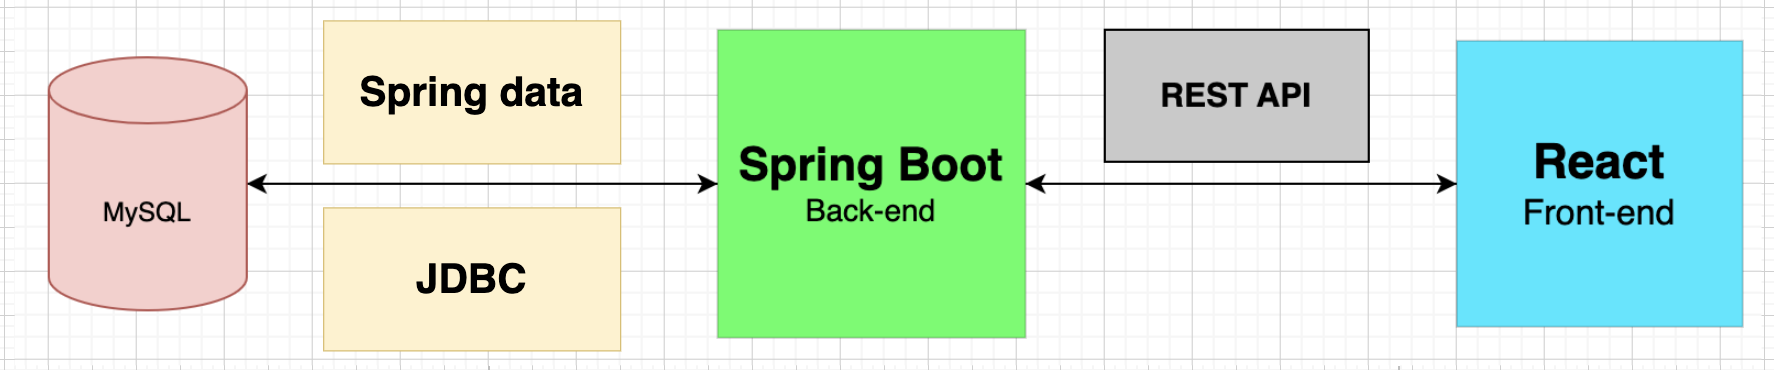
\includegraphics[width=0.9\textwidth]{Images/SpringAndReact.png} 
	\caption{Blockbild der Systemarchitektur} 
	\label{fig:blockbild} 
\end{figure}
\begin{itemize}
	\item \textbf{React Frontend:} Die Benutzeroberfläche wurde mit React umgesetzt. Sie bietet eine moderne, komponentenbasierte Nutzererfahrung. Benutzeraktionen wie Anmeldung, Buchsuche oder Ausleihe werden hier initiiert und über HTTP-Anfragen (im JSON-Format) an die REST-API weitergeleitet.
	
	\item \textbf{REST API:} Die Schnittstelle zwischen Frontend und Backend folgt dem REST-Architekturstil. Die Kommunikation erfolgt über klar definierte Endpunkte unter Verwendung der HTTP-Methoden \texttt{GET}, \texttt{POST}, \texttt{PUT} und \texttt{DELETE}.
	
	\item \textbf{Spring Boot Backend:} Diese Schicht verarbeitet eingehende API-Anfragen, übernimmt die Geschäftslogik, führt Validierungen durch und steuert Datenbankzugriffe. Die Benutzerverwaltung und Zugriffskontrolle erfolgt hier über die Integration mit Okta.
	
	\item \textbf{Spring Data JPA, Spring Data REST und JDBC:} Für den Datenbankzugriff wird Spring Data JPA verwendet, das eine deklarative und effiziente Abfrageerstellung über Repository-Interfaces ermöglicht. Über Spring Data REST werden ausgewählte Repository-Methoden automatisch als REST-Endpunkte bereitgestellt. Intern erfolgt die Kommunikation mit der MySQL-Datenbank über JDBC als Treiberschicht.
	
	\item \textbf{MySQL Database:} Relationale Datenbank zur Speicherung persistenter Daten, strukturiert durch Entitäten wie \texttt{Buch}, \texttt{Rezension} und \texttt{Historie}.
\end{itemize}

\section{UML-Diagramme zur Konzeption}\index{UML}
Zur Visualisierung des Systemkonzepts werden im Folgenden zentrale UML-Diagramme vorgestellt.

\subsection{Klassendiagramm}\index{Klassendiagramm}

Die Abbildung \ref{fig:class_diagram} zeigt das Klassendiagramm der Anwendung \textit{LibraNova}. Das Diagramm gliedert sich in vier Hauptbereiche: Bibliotheksbereich, Zahlungssystem, Kommunikation und Benutzerverwaltung.


\begin{figure}[H]
	\centering
	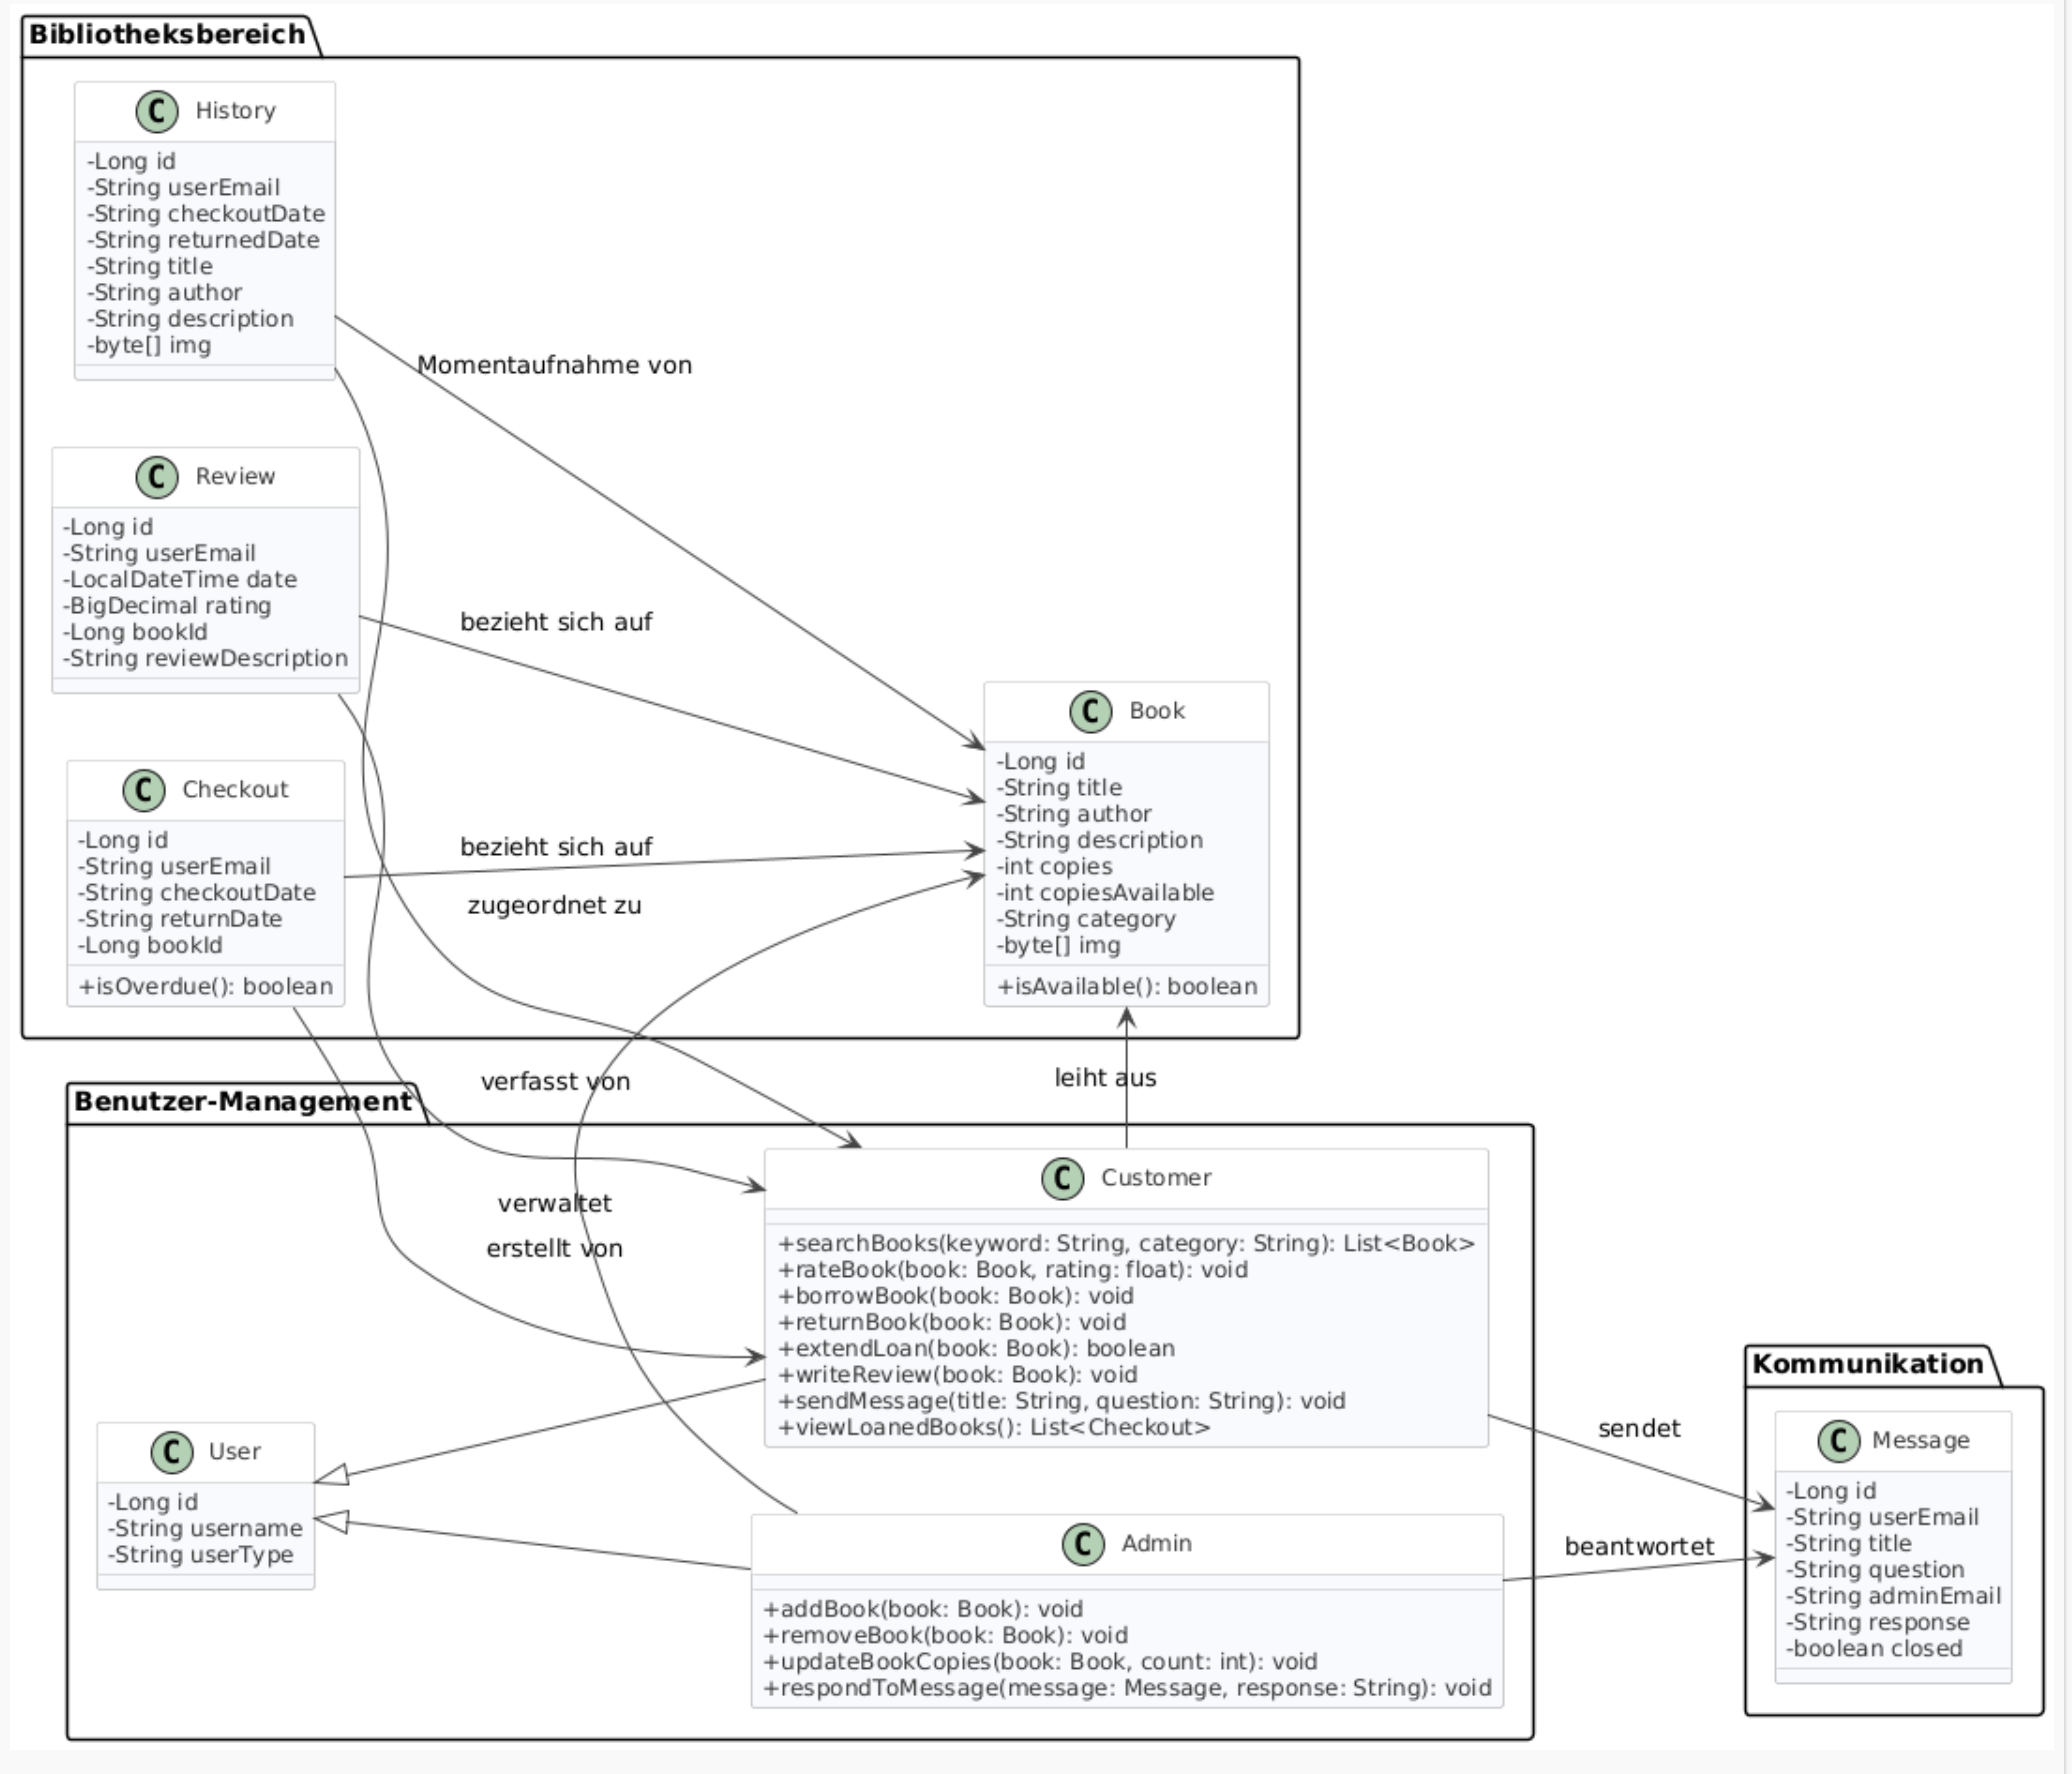
\includegraphics[width=\textwidth]{images/ClassDiagram.png}
	\caption{Klassendiagramm der Anwendung \textit{Libranova}}
	\label{fig:class_diagram}
\end{figure}

\noindent Im Bibliotheksbereich repräsentiert die Klasse \texttt{Book} zentrale Buchinformationen. \texttt{Checkout} modelliert aktive Ausleihen, während \texttt{History} abgeschlossene Ausleihen als Momentaufnahme speichert und auf den \texttt{Checkout}-Vorgängen basiert. Nutzerbewertungen werden über die Klasse \texttt{Review} abgebildet, die einem Buch zugeordnet und von einem \texttt{Customer} erstellt wird.

\noindent Das Zahlungssystem besteht aus den Klassen \texttt{Payment} und \texttt{PaymentHistory}. \texttt{Payment} speichert einzelne Zahlungsinformationen, während \texttt{PaymentHistory} auf diesen Zahlungen aufbaut und dem Nutzer einen Überblick über seine bisherigen Transaktionen bietet.

\noindent Die Kommunikation zwischen Nutzern und Administratoren wird durch die Klasse \texttt{Message} modelliert. Kunden können Nachrichten an Administratoren senden, die diese beantworten.

\noindent Im Bereich Benutzerverwaltung werden die Rollen \texttt{Customer} und \texttt{Admin} dargestellt. \texttt{Admin} verwaltet Bücher und beantwortet Nachrichten, während \texttt{Customer} Bücher ausleiht, bewertet, Nachrichten versendet und Zahlungen tätigt. Die Klassen sind eng über Beziehungen verknüpft: \texttt{Review} und \texttt{Checkout} beziehen sich auf \texttt{Book} und \texttt{Customer}, \texttt{History} basiert auf \texttt{Checkout}-Daten, und \texttt{PaymentHistory} baut auf \texttt{Payment}-Vorgängen auf.

\noindent Das Diagramm verdeutlicht die logische Struktur der Anwendung, die Verantwortlichkeiten der Klassen und die Interaktionen zwischen den Systemkomponenten.

\subsection{Sequenzdiagramme}

Abbildung \ref{fig:Sequence-Diagram} zeigt das Sequenzdiagramm des Benutzer-Login-Vorgangs innerhalb der Anwendung. Ziel dieses Prozesses ist die sichere Authentifizierung des Benutzers sowie die Bereitstellung eines Access Tokens, das den Zugriff auf geschützte Ressourcen ermöglicht.

\begin{figure}[H]
	\centering
	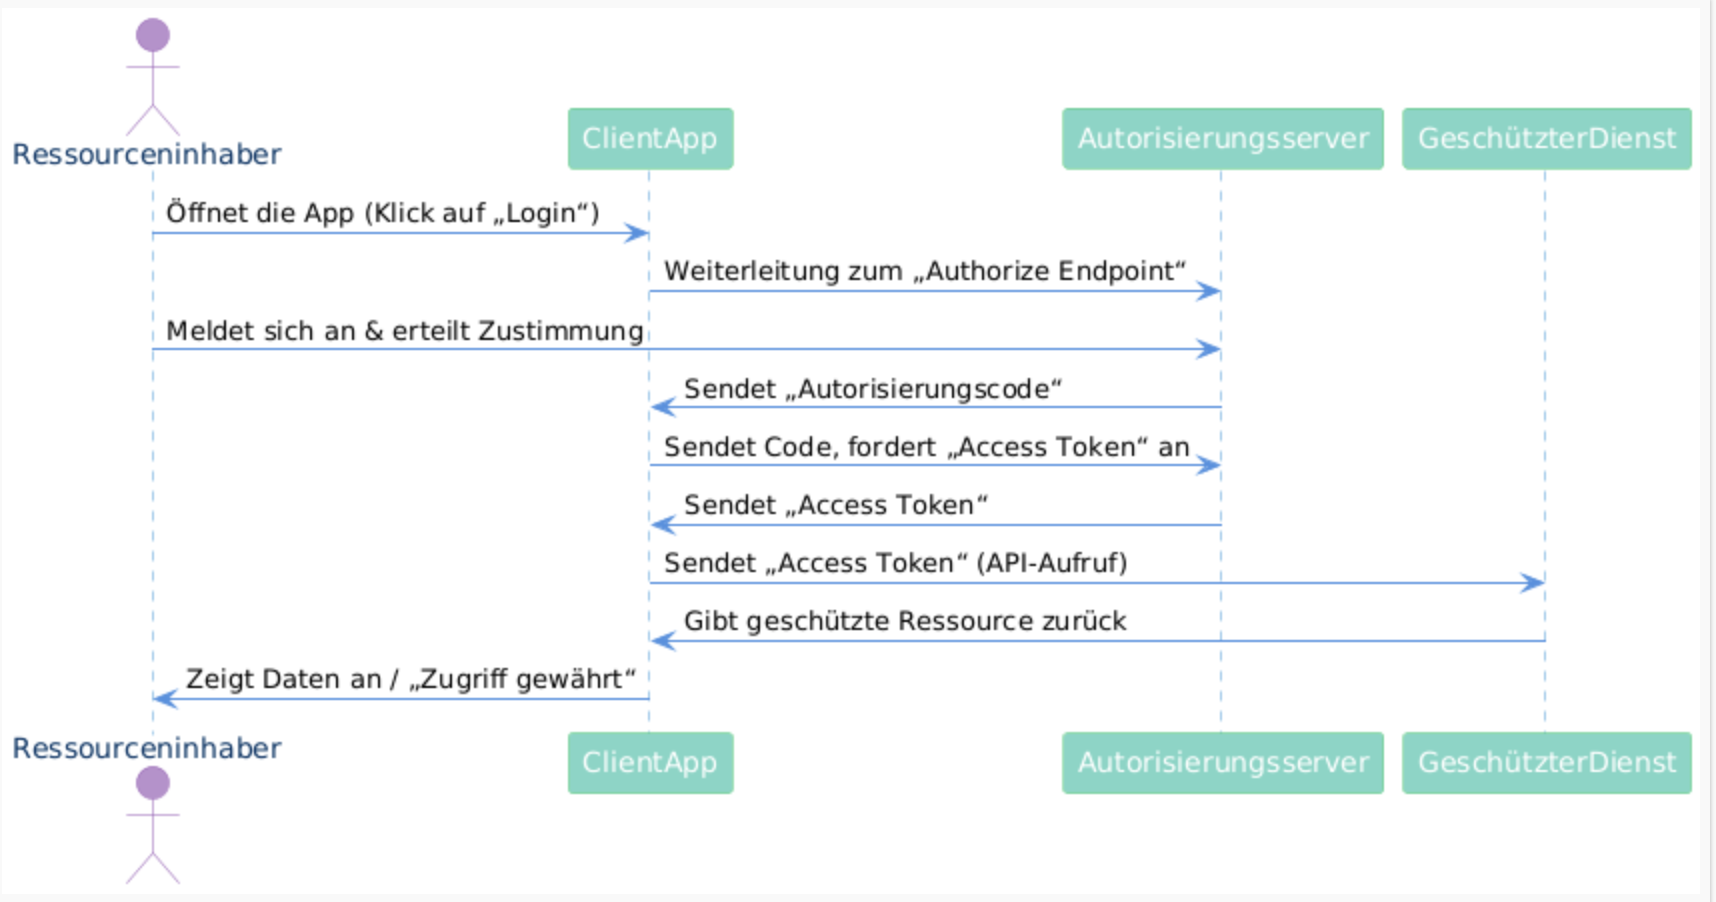
\includegraphics[width=\textwidth]{images/SequenceDiagram.jpg}
	\caption{Sequenzdiagramm des Login-Vorgangs, angelehnt an \cite{OKTALOGIN2025}}
	\label{fig:Sequence-Diagram} 
\end{figure} 

\noindent Im Login-Prozess sind mehrere Komponenten beteiligt. Der Ressourceninhaber (Benutzer) startet den Anmeldevorgang und erteilt die Zustimmung zur Autorisierung. Die Client-Anwendung (React) fungiert als Schnittstelle zwischen Benutzer und System. Der Autorisierungsserver (Okta) authentifiziert den Benutzer, stellt einen Autorisierungscode aus und tauscht diesen gegen ein Access Token ein. Schließlich überprüft der Ressourcenserver (Spring Boot) die Gültigkeit des Tokens und stellt bei erfolgreicher Authentifizierung die geschützten Ressourcen bereit.

\noindent Der Ablauf gliedert sich in folgende Schritte: Zunächst öffnet der Benutzer die React-Anwendung und startet den Login-Prozess. Die Client-Anwendung leitet den Benutzer an den Autorisierungsserver weiter, wo sich der Benutzer anmeldet und der Autorisierung zustimmt. Anschließend sendet der Autorisierungsserver einen Autorisierungscode an die Client-Anwendung, welcher gegen ein Access Token eingetauscht wird. Dieses Token wird lokal gespeichert. Bei einem geschützten API-Aufruf wird das Token an den Ressourcenserver übermittelt. Der Server prüft die Gültigkeit des Tokens und gibt bei erfolgreicher Prüfung die geschützten Daten an die Client-Anwendung zurück, sodass sie dem Benutzer angezeigt werden.

\noindent Nach der Beschreibung der Benutzeranmeldung wird nun der Bezahlvorgang über Stripe betrachtet.

\noindent Abbildung \ref{fig:Stripe-Zahlungsablauf} zeigt den Ablauf eines Bezahlvorgangs mit Stripe. Das Sequenzdiagramm verdeutlicht, wie die React-Anwendung, das Spring Boot-Backend und der externe Zahlungsdienstleister Stripe zusammenwirken, um einen sicheren und effizienten Zahlungsprozess zu gewährleisten.

\begin{figure}[H]
	\centering
	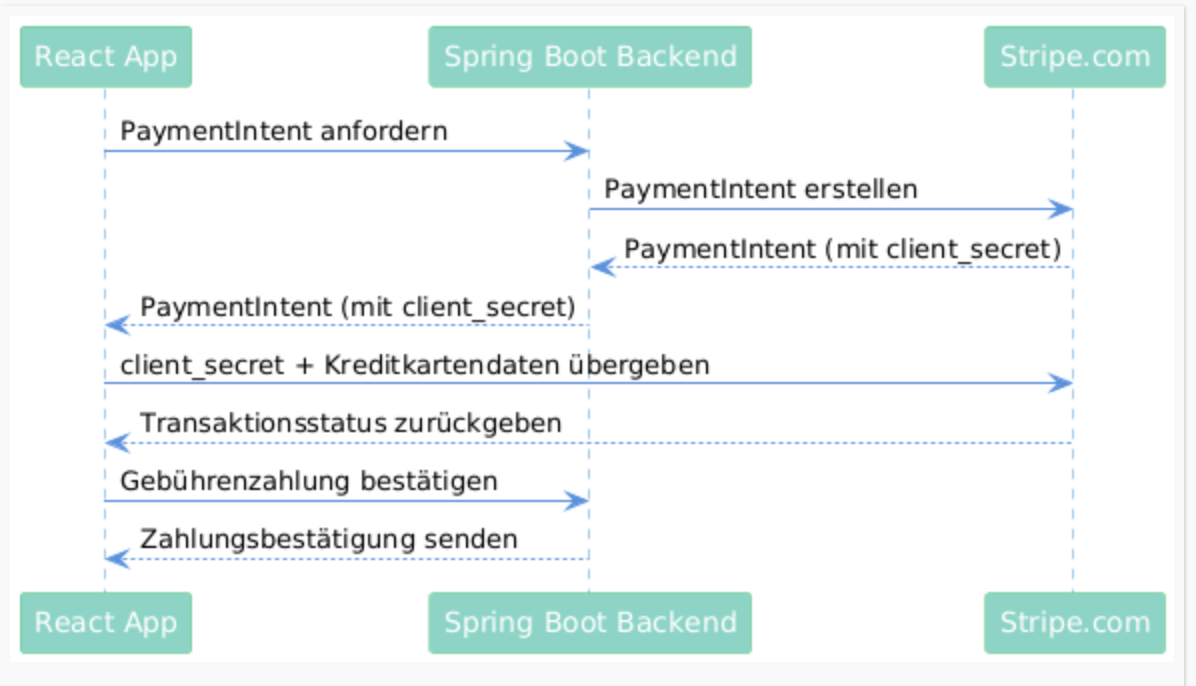
\includegraphics[width=\textwidth]{images/SequenceDiagram-Stripe.png}
	\caption{Zahlungsablauf mit Stripe, angelehnt an \cite{STRIPEAPIFLOW2025}}
	\label{fig:Stripe-Zahlungsablauf} 
\end{figure} 

\noindent Der Zahlungsprozess beginnt, wenn die React-Anwendung eine Anfrage an den Backend-Endpunkt \texttt{/api/payments/secure/intent} sendet, um einen neuen \textit{PaymentIntent} zu erstellen. Das Backend leitet diese Anfrage an Stripe weiter und übermittelt dabei die erforderlichen Parameter wie Betrag, Währung und Zahlungsmethode. Stripe generiert daraufhin einen neuen \textit{PaymentIntent} und gibt diesen, inklusive des \textit{client\_secret}, an das Backend zurück. Das Backend sendet den \textit{client\_secret} an die React-Anwendung, die ihn zusammen mit den Kreditkartendaten direkt an Stripe übermittelt. Stripe verarbeitet die Zahlungsinformationen und gibt den Transaktionsstatus zurück an das Frontend. Abschließend informiert das Frontend das Backend über die erfolgreiche Zahlung, sodass Datenbanken aktualisiert oder Zahlungshistorien gepflegt werden können, und das Backend bestätigt die erfolgreiche Zahlungsabwicklung.

\noindent Ein \textit{PaymentIntent} ist ein von Stripe bereitgestelltes Objekt, das die Absicht einer Zahlung repräsentiert und den gesamten Zahlungsablauf verwaltet – von der Erstellung über die Authentifizierung bis hin zur endgültigen Bestätigung der Zahlung.

\noindent Der \textit{client\_secret} ist ein einzigartiger, von Stripe generierter Schlüssel für jeden \textit{PaymentIntent}. Er dient als sicherer Zugriffstoken, mit dem das Frontend bestimmte Informationen über die jeweilige Zahlung abrufen kann, beispielsweise den aktuellen Status der Transaktion. Der \textit{client\_secret} ist ausschließlich auf diese eine Zahlung beschränkt und kann nicht für andere Aktionen verwendet werden. 

\noindent Der Endpunkt \texttt{POST /api/payments/secure/intent} nimmt ein JSON-Objekt mit Zahlungsinformationen wie Betrag und Währung entgegen. Intern ruft der Controller die Methode \texttt{generatePaymentIntent()} auf, die über das Stripe-SDK einen neuen \textit{PaymentIntent} erstellt. Dabei werden der Betrag (\texttt{amount}), die Währung (\texttt{currency}) und der Zahlungstyp (auf Kreditkarte beschränkt) festgelegt. Das vom Stripe-SDK zurückgegebene \textit{PaymentIntent}-Objekt, inklusive \textit{client\_secret}, wird anschließend vom Backend an das Frontend übermittelt, um den Bezahlvorgang fortzusetzen.

\section{Anforderungen an das System}\index{Systemanforderungen}

Die folgenden Unterabschnitte beschreiben die zentralen Anforderungen an das System. Dazu zählen funktionale, nicht-funktionale sowie technische Anforderungen, die für eine strukturierte Umsetzung der Anwendung erforderlich sind.

\subsection{Funktionale Anforderungen}\index{Funktionale Anforderungen}


Funktionale Anforderungen definieren, welche Dienste das System leisten soll und wie es sich bei bestimmten Eingaben oder in bestimmten Situationen verhalten soll.

\noindent Die wichtigsten funktionalen Anforderungen von \textit{LibraNova} sind:
\begin{itemize}
	\item \textbf{Buchverwaltung:} Nutzer können Bücher suchen, deren Verfügbarkeit prüfen, ausleihen, zurückgeben, verlängern sowie Rezensionen und Bewertungen verfassen.  
	\item \textbf{Administrationsfunktionen:} Administratoren können Bücher hinzufügen, bearbeiten (z.\,B. Anzahl der Exemplare ändern) und aus dem Katalog löschen.  
	\item \textbf{Benutzerfunktionen:} Nutzer können ihre Ausleihen und die Ausleihhistorie einsehen und Zahlungen über Stripe abwickeln.  
	\item \textbf{Such- und Filterfunktionen:} Das System bietet eine Suche nach Titel oder Kategorie, zeigt die Ergebnisse paginiert an und unterstützt eine mehrsprachige Anzeige der Buchbeschreibungen (Deutsch/Englisch).  
	\item \textbf{Systemfeedback:} Das System informiert über nicht verfügbare Bücher, gelöschte Medien in der Ausleihliste sowie über Gebühren bei verspäteter Rückgabe.  
\end{itemize}

\noindent Eine vollständige Übersicht aller funktionalen Anforderungen befindet sich in Anhang \ref{tab:functional-requirements}.

\subsection{Nicht-funktionale Anforderungen}\index{Nicht-funktionale Anforderungen}

Nicht-funktionale Anforderungen beschreiben die Qualitätsmerkmale und Randbedingungen des Systems, wie etwa Leistung, Sicherheit, Benutzbarkeit und Zuverlässigkeit.

\noindent Die wichtigsten nicht-funktionalen Anforderungen von \textit{LibraNova} sind:

\begin{itemize}
	\item \textbf{Benutzerfreundlichkeit:} Die Anwendung muss eine konsistente, intuitive und responsive Benutzeroberfläche bieten, die auf verschiedenen Geräten, Bildschirmgrößen und gängigen Browsern funktioniert. Zudem wird eine zweisprachige Oberfläche (Deutsch/Englisch) bereitgestellt.  
	\item \textbf{Sicherheit:} Sichere Kommunikation über HTTPS, Schutz durch gültige Tokens, klare Trennung von Benutzerrollen sowie Zugriffsbeschränkung auf geschützte Endpunkte.  
	\item \textbf{Leistung:} Such- und Filterfunktionen sowie Login-Vorgänge müssen kurze Reaktionszeiten gewährleisten, um eine flüssige Nutzung zu ermöglichen.  
	\item \textbf{Barrierefreiheit:} Erfüllung grundlegender WCAG-2.1-Anforderungen (Level AA), um auch Nutzern mit Einschränkungen einen Zugang zu ermöglichen.  
	\item \textbf{Wartbarkeit und Erweiterbarkeit:} Modularer Aufbau der Backend-Services sowie eine aktuelle und entwicklerfreundliche API-Dokumentation.  
\end{itemize}

\noindent Eine vollständige Übersicht aller nicht-funktionalen Anforderungen befindet sich in Anhang \ref{tab:non-functional-requirements}.

\subsection{Technische  Anforderungen}\index{Technische Anforderungen}

Technische Anforderungen beschreiben, welche Technologien, Werkzeuge und Methoden für die Entwicklung und den Betrieb von LibraNova verwendet werden. Dazu gehören zum Beispiel Programmiersprachen, Frameworks, Schnittstellen und Protokolle.

\noindent Die wichtigsten technischen Anforderungen von \textit{LibraNova} sind:
\begin{itemize}
	\item \textbf{Architektur:} Spring Boot als Backend mit RESTful APIs, React als Frontend sowie eine relationale MySQL-Datenbank für die Persistenz.  
	\item \textbf{Sicherheit und Authentifizierung:} HTTPS, JWT-Token, OAuth2/OpenID Connect mit Okta sowie CORS-Restriktionen für das vertrauenswürdige Frontend.  
	\item \textbf{Entwicklung und Qualitätssicherung:} Nutzung von Spring Data JPA/REST, Swagger-Dokumentation, Lombok sowie Unit-Tests mit JUnit und Mockito.  
\end{itemize}

\noindent Eine vollständige Übersicht aller technischen Anforderungen befindet sich in Anhang \ref{tab:technical-requirements}.

\section{Wichtige Algorithmen (Pseudocode)}\index{Algorithmen}

In diesem Abschnitt werden die wichtigsten Algorithmen dargestellt, die zentrale Abläufe des Systems beschreiben. Die Abläufe werden aus der Perspektive der Benutzerinteraktionen sowie der dahinterliegenden Systemlogik erläutert. Dabei werden wesentliche Prüfungen und Bedingungen berücksichtigt, um einen klaren und nachvollziehbaren Überblick über die Funktionsweise zu geben.

\subsection{Buchausleihe}\index{Buchausleihe}

Der folgende Pseudocode \ref{lst:buchausleihe} beschreibt den vollständigen Ablauf der Buchausleihe aus der Perspektive des Benutzers sowie der Systemlogik. Dabei werden wichtige Prüfungen berücksichtigt, wie die Anmeldung des Benutzers, die Verfügbarkeit von Exemplaren, die maximale Anzahl ausgeliehener Bücher sowie etwaige überfällige Rückgaben oder offene Gebühren.

\begin{lstlisting}[style=pseudocode, caption={Pseudocode für den Ausleihvorgang eines Buches}, label={lst:buchausleihe}]
	1.  Benutzer öffnet die Detailseite eines Buches.
	2.  System prüft:
	     a. Ist der Benutzer angemeldet?
	         - Nein → Zeige Button >> Anmelden << (Weiterleitung zur Login-Seite)
	         - Ja → Weiter zu Schritt 3
	3.  Hat der Benutzer dieses Buch bereits ausgeliehen?
	         - Ja → Zeige Hinweis >> Bereits ausgeliehen <<
	         - Nein → Weiter zu Schritt 4
	4.  Hat der Benutzer weniger als 5 Bücher ausgeliehen?
	        - Nein → Zeige Hinweis >> Maximale Anzahl an Büchern erreicht <<
	        - Ja → Weiter zu Schritt 5
	5.  Sind Exemplare des Buches verfügbar?
         	- Nein → Zeige deaktivierten Button >> Ausleihen <<
	        - Ja → Zeige aktiven Button >> Ausleihen <<
	6.  Klickt der Benutzer auf >> Ausleihen <<:
	     a. Hat der Benutzer überfälligen Bücher oder unbezahlten Gebühren?
	         - Nein → Lege Ausleiheintrag in der Datenbank an (7 Tage Leihfrist) 
	         - Ja → Zeige Meldung: >> Bitte geben Sie überfällige Bücher zurück und begleichen Sie offene Gebühren, bevor Sie neue Bücher ausleihen können. <<
\end{lstlisting}


\subsection{Verlängerung der Buchausleihe}\index{Verlängerung der Buchausleihe}

Der folgende Pseudocode \ref{lst:extend-loan} beschreibt den vollständigen Ablauf, wie Nutzer die Leihfrist eines ausgeliehenen Buches verlängern können. Dabei werden die Bedingungen geprüft, unter denen eine Verlängerung möglich ist, sowie die Benutzeroberfläche entsprechend angepasst.

\begin{lstlisting}[style=pseudocode, caption={Pseudocode für die Verlängerung einer Buchausleihe}, label={lst:extend-loan}]
	1.  Benutzer öffnet seine Ausleihen und klickt bei einem Buch auf >> Ausleihe verwalten <<.
	2.  System zeigt zwei Optionen:
	     a. >> Zurückgeben <<
	     b. >> Verlängern <<
	3.  System prüft für den Button >> Verlängern <<:
	     a. Ist das Rückgabedatum überschritten?
	     b. Wurde das Buch aus dem System gelöscht?
	4.  Wenn eine der Bedingungen erfüllt ist:
	     a. Zeige deaktivierten Button mit dem Text >> Verlängerung nicht möglich <<.
	5.  Wenn keine der Bedingungen zutrifft:
	     a. Button >> Verlängern << ist aktiv.
	     b. Benutzer klickt auf >> Verlängern <<.
	     c. System verlängert die Leihfrist um 7 Tage.
	     d. Verbleibende Tage werden aktualisiert.
\end{lstlisting}


























\chapter{Realisierung}

In diesem Kapitel werden die zentralen Komponenten der Systemarchitektur vorgestellt. Es beginnt mit dem modular aufgebauten Backend auf Basis von Spring Boot, gefolgt von der Struktur und Internationalisierung des Frontends mit React. Abschließend wird das Datenbankmodell erläutert, einschließlich der Persistenzlogik mit Spring Data und Hibernate.

\section{Backend-Architektur}\index{Backend-Architektur}
 
Das Backend basiert auf Spring Boot und folgt einer klar strukturierten, modularen Architektur. Beschrieben werden der Einstiegspunkt, die Paketstruktur sowie die eingesetzte Teststrategie zur Sicherstellung der Codequalität.

\subsection{Projektinitialisierung und Startklasse}\index{Projektinitialisierung}

Spring Boot vereinfacht die Entwicklung von Java-basierten Webanwendungen durch konventionsbasierte und automatisierte Projektkonfiguration. Dieses Framework bietet eine standardisierte Struktur, automatisches Abhängigkeitsmanagement und integrierte Komponenten, die den Entwicklungsprozess erheblich beschleunigen.

\noindent In diesem Abschnitt wird die Struktur des Projekts erläutert, wobei der Schwerpunkt auf der Projektinitialisierung, den zentralen Einstiegspunkt der Anwendung sowie wesentliche Konfigurationsmechanismen liegt.
\begin{itemize}
	\item \textbf{Projektinitialisierung (Spring Initializr):} Die Anwendung \textit{LibraNova} wurde mithilfe des Online-Tools \textit{Spring Initializr} (\url{https://start.spring.io/}) erzeugt. Dieses Tool ermöglicht die einfache Auswahl von Projektparametern wie Abhängigkeiten, Java-Version und Build-Tool (z.\,B. Maven oder Gradle) und generiert eine startbereite Projektstruktur inklusive grundlegender Dateien und Verzeichnisse.
	
	\item \textbf{Einstiegspunkt der Anwendung – Main-Klasse:} Die zentrale Einstiegsklasse der Anwendung befindet sich im \texttt{src/main/java}-Verzeichnis und enthält die \texttt{main}-Methode. Sie ist mit der Annotation \texttt{@SpringBootApplication} versehen, welche drei wichtige Spring-Annotationen kombiniert:
	\begin{itemize}
		\item \texttt{@Configuration} – Kennzeichnet die Klasse als Quelle für Bean-Definitionen.
		\item \texttt{@EnableAutoConfiguration} – Aktiviert die automatische Konfiguration basierend auf den eingebundenen Abhängigkeiten.
		\item \texttt{@ComponentScan} – Ermöglicht das automatische Auffinden von Komponenten, Services und Repositories im angegebenen Paket und dessen Unterpaketen.
	\end{itemize}
	
	Nachfolgend \ref{lst:springboot-main} ist der Quellcode der Main-Klasse dargestellt:
	
	\begin{lstlisting}[language=Java, caption=Einstiegspunkt der Spring Boot Anwendung, label=lst:springboot-main, breaklines=true]
		@SpringBootApplication
		public class SpringBootLibraryApplication {
			
			public static void main(String[] args) {
				SpringApplication.run(SpringBootLibraryApplication.class, args);
			}
			
		}
	\end{lstlisting}

  \noindent \textit{Erläuterung der Main-Klasse:}
  \begin{itemize}
  	\item \texttt{@SpringBootApplication}: Diese Annotation bündelt die Konfiguration, Auto-Konfiguration und Komponentensuche in einer einzigen Annotation und ist der zentrale Startpunkt für die Spring-Boot-Anwendung.
  	\item \texttt{public class SpringBootLibraryApplication}: Definition der Hauptklasse, die die Anwendung repräsentiert.
  	\item \texttt{public static void main(String[] args)}: Die Main-Methode dient als Einstiegspunkt der Java-Anwendung. Sie wird beim Programmstart aufgerufen.
  	\item \texttt{SpringApplication.run(...) }: Diese Methode startet den eingebetteten Server, initialisiert den Spring Application Context und lädt alle Komponenten, Beans und Konfigurationen.
  \end{itemize}

\item \textbf{Konfiguration über \texttt{application.properties}:} Die Datei \texttt{application.properties} im Verzeichnis \texttt{src/main/resources} enthält zentrale Konfigurationen der Anwendung, wie z.\,B. Datenbankverbindung, REST-Basis-Pfad und andere anwendungsspezifische Einstellungen.

\begin{lstlisting}[language=, caption=Beispielhafte application.properties Datei, label=lst:application-properties, breaklines=true]
	# Name der Anwendung
	spring.application.name=libranova
	
	# Datenbankverbindung (MySQL)
	spring.datasource.url=jdbc:mysql://localhost:3306/libranova_db
	spring.datasource.username=username
	spring.datasource.password=password
	
	# Dialekt von Hibernate
	spring.jpa.properties.hibernate.dialect=org.hibernate.dialect.MySQLDialect
	
	# Basis-REST-Pfad
	spring.data.rest.base-path=/api
\end{lstlisting}

\textit{Erläuterung der wichtigsten Einstellungen:}
\begin{itemize}
	\item \texttt{spring.application.name}: Definiert den Namen der Anwendung, z.\,B. für Logs oder Monitoring.
	\item \texttt{spring.datasource.url}: Verbindungs-URL zur MySQL-Datenbank inklusive Host, Port und Datenbankname.
	\item \texttt{spring.datasource.username}: Benutzername für die Datenbankverbindung.
	\item \texttt{spring.datasource.password}: Passwort für den Datenbankzugang.
	\item \texttt{spring.jpa.properties.hibernate.dialect}: Gibt den SQL-Dialekt für JPA/Hibernate an (hier MySQL).
	\item \texttt{spring.data.rest.base-path}: Legt den Basis-URL-Pfad für automatisch generierte REST-Endpunkte fest (z.\,B. \texttt{/api}).
\end{itemize}

\item \textbf{Eingebetteter Webserver (Tomcat):} Spring Boot integriert standardmäßig einen eingebetteten Webserver (standardmäßig Tomcat). Dadurch kann die Anwendung direkt als eigenständiger Prozess gestartet werden, ohne dass ein separater Webserver installiert oder konfiguriert werden muss \cite{SPRINGBOOT2025b}.
\end{itemize}

\subsection{Modulare Paketstruktur des Backends}\index{Paketstruktur}
Im Folgenden wird die interne Struktur des Backends detailliert betrachtet. Dazu gehört die Aufteilung der Anwendung in verschiedene Pakete, die jeweils eigene Verantwortlichkeiten übernehmen und so zur Übersichtlichkeit und Wartbarkeit beitragen.  

\noindent Eine schematische Übersicht der Paketstruktur ist in \textbf{Abbildung~\ref{fig:package-structure}} unten dargestellt.
\begin{figure}[H]
	\centering
	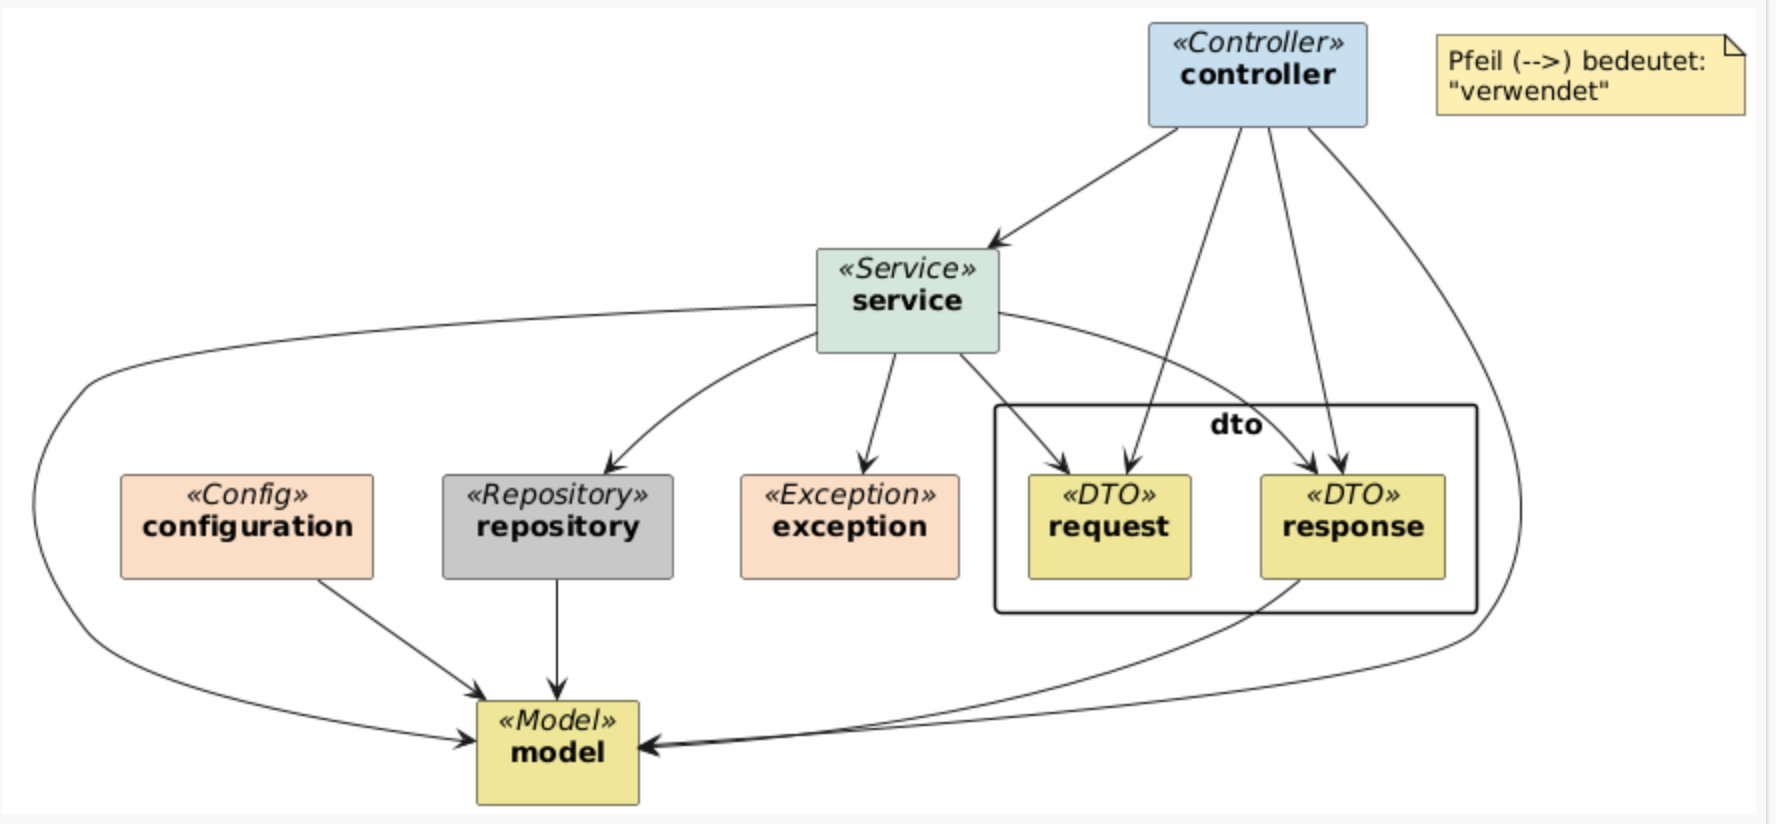
\includegraphics[width=0.99\textwidth]{images/backend_structure.png}
	\caption{Modularer Aufbau des Backends}
	\label{fig:package-structure}
\end{figure} 
\noindent Im Folgenden werden die Pakete und ihre jeweiligen Verantwortlichkeiten beschrieben.
\begin{itemize}
	\item \textbf{model:} Enthält die JPA-Entitäten, die die Tabellen der MySQL-Datenbank abbilden. Jede Klasse in diesem Paket entspricht einer Datenbanktabelle und definiert deren Attribute und Beziehungen. Diese Entitäten bilden die Grundlage für den Datenzugriff über das Repository.
	
	\item \textbf{dto:} Dient dem strukturierten Datenaustausch zwischen Client und Server, ohne interne Entitäten direkt preiszugeben. Es gibt zwei Unterpakete:
	\begin{itemize}
		\item \texttt{request}: definiert Datenstrukturen für eingehende Anfragen wie etwa Formularinhalte oder Suchparameter,
		\item \texttt{response}: definiert Rückgabeformate, die speziell für die Client-seitige Anzeige oder Weiterverarbeitung optimiert sind.
	\end{itemize}
	Die Verwendung von DTOs erhöht die Sicherheit und Flexibilität des Datenmodells.
	
	\item \textbf{exception:} Beinhaltet zentrale Komponenten zur Fehlerbehandlung. In der aktuellen Implementierung ist eine benutzerdefinierte Ausnahme enthalten, die bei nicht verfügbaren Büchern geworfen wird. Diese Ausnahme verbessert die Verständlichkeit von Fehlermeldungen auf der Client-Seite.
	
	\item \textbf{repository:} Beinhaltet Interfaces zur Datenzugriffsabstraktion mittels \texttt{Spring Data JPA}. Sie ermöglichen CRUD-Operationen auf den JPA-Entitäten, ohne dass eigene SQL-Statements geschrieben werden müssen. Damit wird der Datenzugriff stark vereinfacht und typensicher umgesetzt. 
	
	\item \textbf{service:} Kapselt die Geschäftslogik der Anwendung. Hier werden Anfragen aus den Controllern verarbeitet, Daten validiert und Repository-Zugriffe koordiniert. Die Services dienen als zentrale Steuerungseinheit zwischen Controller-Logik und Datenbankzugriff. 
	
	\item \textbf{controller:} Beinhaltet die REST-Controller zur Entgegennahme und Verarbeitung von HTTP-Anfragen. Sie dienen als Schnittstelle zwischen Client und Server und leiten die Anfragen zur weiteren Verarbeitung an die Service-Schicht weiter. Zudem bereiten sie die Daten so auf, dass sie für den Client verständlich und verwertbar sind.
	
	\item \textbf{configuration:} Enthält zentrale Sicherheitskonfigurationen der Anwendung. Hier werden der Zugriff auf HTTP-Endpunkte sowie Authentifizierungsmechanismen mittels JWT und OAuth2 (Okta) definiert und gesteuert.
\end{itemize}

\subsection{Teststrategie und Testintegration}\index{Teststrategie}

Um die Qualität und Zuverlässigkeit des Backends sicherzustellen, wurde ein automatisiertes Testkonzept implementiert. Dabei kommen vor allem Unit-Tests mit \textit{JUnit} sowie Mocking mit \textit{Mockito} zum Einsatz.

\noindent Die Tests befinden sich im Verzeichnis \texttt{src/test/java} und folgen der Paketstruktur des Produktivcodes, um eine klare Zuordnung zu ermöglichen.

\begin{itemize}
	\item \textbf{JUnit} wird verwendet, um einzelne Komponenten isoliert zu testen und deren Verhalten zu validieren.
	\item \textbf{Mockito} ermöglicht das Erzeugen von Mock-Objekten, um Abhängigkeiten während der Tests zu simulieren und somit isolierte Testumgebungen zu schaffen.
\end{itemize}

\noindent Integration der Tests in den Build-Prozess erfolgt über das verwendete Build-Tool \textbf{Maven}, wodurch die Tests automatisiert ausgeführt werden können und eine kontinuierliche Qualitätssicherung gewährleistet ist.


\section{Frontend-Struktur}\index{Frontend-Struktur}

In diesem Abschnitt wird die Architektur des Frontends erläutert. Beginnend mit dem Einstiegspunkt der React-Anwendung, werden anschließend die Projektstruktur sowie die Integration der Internationalisierung mittels i18next vorgestellt.

\subsection{Einstiegspunkt der React-Anwendung}\index{Frontend-Initialisierung}

Das Frontend der Anwendung wurde mit \textbf{React} und \textbf{TypeScript} auf Basis von \textbf{Create React App (CRA)} entwickelt. CRA bietet eine sofort einsatzbereite Entwicklungsumgebung inklusive Webpack-Konfiguration, Hot-Reloading, Testing-Setup und TypeScript-Support \cite{CRA2025}.

\noindent In diesem Abschnitt wird die Struktur der React-Anwendung beschrieben, wobei der Schwerpunkt auf der Projektinitialisierung, dem Einstiegspunkt sowie zentralen Konfigurationsdateien liegt.

\begin{itemize}
	\item \textbf{Projektinitialisierung mit CRA:} Die Anwendung wurde über folgendes Kommando initialisiert (siehe Listing~\ref{lst:cra-init}):
	\begin{lstlisting}[language=bash, caption=Projektinitialisierung mit Create React App, label=lst:cra-init]
		npx create-react-app react-library-app --template typescript
	\end{lstlisting}

Dieses Kommando setzt sich wie folgt zusammen:

\begin{itemize}
	\item \texttt{npx}: Führt ein npm-Paket temporär aus, ohne es global zu installieren.
	\item \texttt{create-react-app}: Das offizielle Tool zur Erzeugung von React-Projekten, welches ein komplettes Setup mit Build-Tooling, Linter und Tests erstellt.
	\item \texttt{react-library-app}: Der Name des Projektverzeichnisses, das automatisch erstellt wird.
	\item \texttt{--template typescript}: Gibt an, dass die Anwendung mit TypeScript anstelle von JavaScript erstellt werden soll.
\end{itemize}

	Dadurch wurde eine vollständige Projektstruktur erzeugt, einschließlich Konfigurationsdateien, TypeScript-Unterstützung und einer initialen Komponentenstruktur.
	
	\item \textbf{Einstiegspunkt – \texttt{index.tsx}:} Die Datei \texttt{src/index.tsx} (siehe Listing~\ref{lst:react-index}) bildet den Einstiegspunkt der React-Anwendung. Dort wird die Hauptkomponente \texttt{<App />} in das DOM eingebunden:
	
	\begin{lstlisting}[language=Java, caption=Einstiegspunkt der React-Anwendung, label=lst:react-index, breaklines=true]
	import React from 'react';
	import ReactDOM from 'react-dom/client';
	import './index.css';
	import { App } from './App';
	import { BrowserRouter } from 'react-router-dom';
	import 'bootstrap-icons/font/bootstrap-icons.css';
	import { loadStripe } from '@stripe/stripe-js';
	import { Elements } from '@stripe/react-stripe-js';
	import './i18n';
	
	const stripePromise = loadStripe('my_stripe_public_key');
	
	const root = ReactDOM.createRoot(
	document.getElementById('root') as HTMLElement
	);
	root.render(
	<BrowserRouter>
	<Elements stripe={stripePromise}>
	<App />
	</Elements>
	</BrowserRouter>
	);
	\end{lstlisting}
	
	Die Datei \texttt{index.tsx} dient als zentrales Einstiegsskript für die React-Anwendung. Sie importiert zunächst alle notwendigen Module und Abhängigkeiten wie React selbst, den ReactDOM-Client, die globale CSS-Datei, die Hauptkomponente \texttt{App} sowie zusätzliche Bibliotheken für Routing (\texttt{react-router-dom}), UI-Icons (Bootstrap Icons), Zahlungsintegration (Stripe) und Internationalisierung (\texttt{i18n}).
	
	Im nächsten Schritt wird Stripe über \texttt{loadStripe} mit dem öffentlichen Schlüssel initialisiert und in einer Promise-Variable gespeichert. Anschließend wird mithilfe von \texttt{ReactDOM.createRoot(...)} eine sogenannte „Root“-Instanz erzeugt, welche das \texttt{<div>} mit der ID \texttt{root} im HTML-Dokument referenziert. Das \texttt{<div>} mit der ID \texttt{root} befindet sich in der Datei \texttt{public/index.html}.
	
	Im letzten Schritt erfolgt das eigentliche Rendern der Anwendung. Hierbei wird die Komponente \texttt{<App />} in den Kontext von \texttt{<BrowserRouter>} und \texttt{<Elements>} eingebettet, um Routing- und Zahlungsfunktionen global bereitzustellen.
	
\item \textbf{Backend-Kommunikation über Umgebungsvariablen:} Hier wird die Port-URL des Backends definiert, welche von der React-Anwendung zur Kommunikation mit dem Backend genutzt wird. Diese Konfiguration erfolgt über die Datei \texttt{.env} (siehe Listing~\ref{lst:cra-env}).  

Die Umgebungsvariable \texttt{REACT\_APP\_API\_URL} gibt die Adresse an, unter der die REST-API des Backends erreichbar ist. Damit diese Variable im Code verwendet werden kann, muss sie zwingend mit dem Präfix \texttt{REACT\_APP\_} beginnen.
Diese Variable wird beispielsweise im Code zur Konfiguration der API-Endpunkte verwendet, z.\,B.\ \texttt{fetch(process.env.REACT\_APP\_API\_URL + '/books')}.


\begin{lstlisting}[language=, caption=Frontend-Umgebungsvariable für Backend-Zugriff in .env-Datei, label=lst:cra-env]
	REACT_APP_API_URL='https://localhost:8443/api'
\end{lstlisting}

	
\end{itemize}

\subsection{React-Projektstruktur}\index{React-Projektstruktur}

Im Folgenden wird die interne Struktur der React-Frontend-Anwendung detailliert betrachtet. Die Anwendung ist in verschiedene Verzeichnisse unterteilt, die jeweils spezifische Verantwortlichkeiten übernehmen und dadurch zur Übersichtlichkeit, Modularität und Wartbarkeit beitragen.

\noindent Eine schematische Übersicht der Verzeichnisse und zentralen Dateien ist in \textbf{Abbildung~\ref{fig:folder-structure}} unten dargestellt.
\begin{figure}[H]
	\centering
	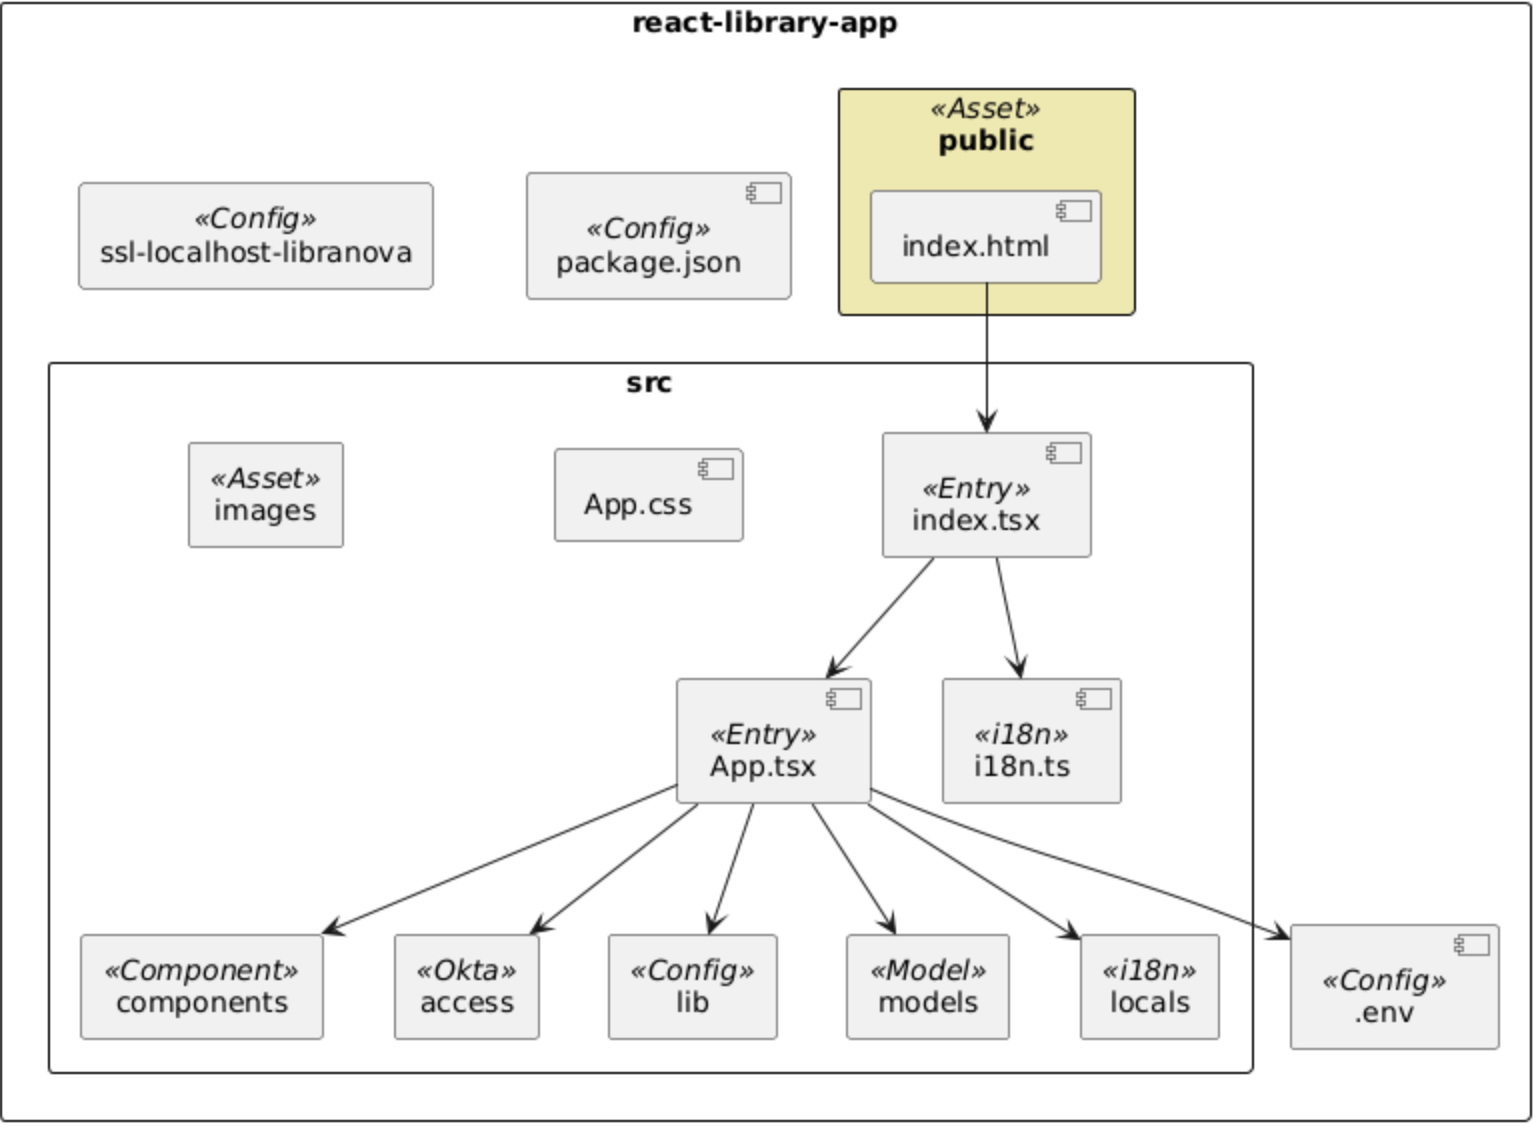
\includegraphics[width=1.00\textwidth]{images/frontend_structure.png}
	\caption{Modularer Aufbau des Frontends}
	\label{fig:folder-structure}
\end{figure} 
\noindent Anschließend werden die wichtigsten Ordner und Dateien sowie ihre jeweiligen Aufgabenbereiche beschrieben.
\begin{itemize}
	\item \textbf{index.html:} Statisches HTML-Grundgerüst der Anwendung. Enthält das \texttt{<div>} mit der ID \texttt{root}, in das React die App rendert. Zusätzlich werden hier externe Ressourcen wie Bootstrap und Stripe eingebunden.
	
	\item \textbf{package.json:} Zentrale Konfigurationsdatei für das React-Projekt. Definiert alle Projektabhängigkeiten, Skripte zur Ausführung (z.\,B.\ Starten, Bauen, Testen), sowie weitere Metadaten der Anwendung.
	
	\item \textbf{ssl-local-libranova:} Enthält SSL-Zertifikat (\texttt{localhost.crt}) und privaten Schlüssel (\texttt{localhost.key}) für die lokale HTTPS-Entwicklung.
	
	\item \textbf{index.tsx:} (siehe Listing~\ref{lst:react-index}) — bereits zuvor beschrieben im Abschnitt zur Einstiegspunktstruktur.
	
	\item \textbf{App.css:} Enthält benutzerdefinierte globale CSS-Regeln zur Gestaltung zentraler UI-Komponenten, darunter Header, Buttons, Bilder, Effekte sowie Media Queries zur responsiven Darstellung.
	
	\item \textbf{images:} Enthält statische Bilddateien, die in der Benutzeroberfläche verwendet werden.
	
	\item \textbf{i18n.ts:} Initialisiert die Mehrsprachigkeit mittels \texttt{i18next} mit englischen und deutschen Übersetzungen sowie automatischer Sprachenerkennung.
	
	\item \textbf{App.tsx:}  
	Zentrale Komponente der Anwendung, die das Routing und die Navigation steuert.  
	Sie bindet verschiedene Seiten und Komponenten ein und integriert die Authentifizierung mit Okta.  
	Header und Footer sorgen für das Layout, während geschützte Routen durch \texttt{Security} verwaltet werden.
	
	\item \textbf{components:}  
	Enthält die wiederverwendbaren UI-Komponenten der Anwendung, wie Header, Footer, Hauptseite, Suchseite und weitere funktionale Elemente.  
	Diese Komponenten bilden die Benutzeroberfläche und sind modular aufgebaut, um Wartbarkeit und Erweiterbarkeit zu gewährleisten.
	
	\item \textbf{access:}  
	Beinhaltet die Integration und Steuerung des Okta-Authentifizierungswidgets.  
	Die Komponenten \texttt{OktaLoginWidget} und \texttt{OktaSigninWidget} ermöglichen das Anmelden, Handhaben von Login-Events und Weiterleitung nach erfolgreicher Authentifizierung.  	
	
	\item \textbf{lib:}  
	Enthält die Datei \texttt{oktaConfig.ts}, die die Einstellungen für die Okta-Authentifizierung definiert, wie Client-ID, Autorisierungsserver (Issuer), Redirect-URI und Berechtigungen (Scopes).  
	Diese Konfiguration ist zentral für die Anbindung der Okta-Authentifizierung im Frontend.
	
	\item \textbf{models:}  
	Enthält Klassen, die zentrale Datenstrukturen der Anwendung modellieren, wie z.\,B. \texttt{Book}.  
	Sie dienen als Grundlage für den strukturierten Datenaustausch innerhalb des Frontends sowie zwischen Frontend und Backend.
	
	\item \textbf{locales:}  
	Beinhaltet sprachspezifische JSON-Dateien (\texttt{en}, \texttt{de}) für die Internationalisierung der UI mittels \texttt{react-i18next}.
	
	\item \textbf{.env:}  
	Diese Datei definiert Umgebungsvariablen für das Projekt.  
	Dazu gehören Pfade zu SSL-Zertifikat und -Schlüssel für die HTTPS-Kommunikation im lokalen Entwicklungsumfeld sowie die Backend-URL (\texttt{REACT\_APP\_API\_URL}) für die React-Anwendung.

\end{itemize}

\subsection{Internationalisierung mit i18next}\index{Internationalisierung mit i18next}

Zur Umsetzung der Mehrsprachigkeit im Frontend wurde das \texttt{i18next}-Framework in Kombination mit \texttt{react-i18next} und \texttt{i18next-browser-languagedetector} verwendet. Nach der Installation dieser Abhängigkeiten wird in der Datei \texttt{i18n.ts} (siehe Listing~\ref{lst:i18n.ts}) die Initialisierung des Übersetzungssystems vorgenommen.


\begin{lstlisting}[style=pseudocode, caption={Initialisierung von i18next in \texttt{i18n.ts}}, label={lst:i18n.ts}, breaklines=true]
import i18n from "i18next";
import { initReactI18next } from "react-i18next";
import LanguageDetector from "i18next-browser-languagedetector";

import translationEN from "./locales/en/translation.json";
import translationDE from "./locales/de/translation.json";

const resources = {
	en: { translation: translationEN },
	de: { translation: translationDE }
};

i18n
.use(LanguageDetector)  // Detektiert die Sprache des Benutzers
.use(initReactI18next) // Bindet i18next an React
.init({
	resources,
	fallbackLng: "en", // verwenden Sie Englisch als Fallback-Sprache
	interpolation: {
		escapeValue: false // React bereits vor XSS-Angriffen schützt
	}
});

export default i18n;
\end{lstlisting}

\noindent Hier ist eine Zeile-für-Zeile-Erklärung der Datei \texttt{i18n.ts}, die die Internationalisierung der React-Anwendung initialisiert:

\begin{itemize}
	\item \texttt{import i18n from "\texttt{i18next}";} \\
	Importiert die Hauptbibliothek \texttt{i18next}, die die Internationalisierung ermöglicht.
	
	\item \texttt{import \{ initReactI18next \} from "react-i18next";} \\
	Importiert die React-spezifische Integration, um \texttt{i18next} mit React zu verbinden.
	
	\item \texttt{import LanguageDetector from " \texttt{i18next}-browser-languagedetector";} \\
	Importiert ein Modul zur automatischen Erkennung der Sprache des Benutzers im Browser.
	
	\item \texttt{import translationEN from "./locales/en/translation.json";} \\
	Importiert die englischen Übersetzungen aus der JSON-Datei.
	
	\item \texttt{import translationDE from "./locales/de/translation.json";} \\
	Importiert die deutschen Übersetzungen aus der JSON-Datei.
	
	\item \texttt{const resources = \{} \\
	\hspace{1em} \texttt{en: \{ translation: translationEN \},} \\
	\hspace{1em} \texttt{de: \{ translation: translationDE \}} \\
	\texttt{\};} \\
	Definiert die verfügbaren Sprachressourcen mit den jeweiligen Übersetzungen.
	
	\item \texttt{i18n} \\
	\hspace{1em} \texttt{.use(LanguageDetector)} \\
	\hspace{1em} \texttt{.use(initReactI18next)} \\
	\hspace{1em} \texttt{.init(\{} \\
	\hspace{2em} \texttt{resources,} \\
	\hspace{2em} \texttt{fallbackLng: "en",} \\
	\hspace{2em} \texttt{interpolation: \{} \\
	\hspace{3em} \texttt{escapeValue: false} \\
	\hspace{2em} \texttt{\}} \\
	\hspace{1em} \texttt{\});} \\
	Initialisiert \texttt{i18next} mit: automatischer Spracherkennung, React-Integration, Sprachressourcen, Standard-Fallbacksprache Englisch, und deaktiviert Escape-Mechanismen, da React bereits sicher ist.
	
	\item \texttt{export default i18n;} \\
	Exportiert die konfigurierte Instanz, damit sie im Projekt verwendet werden kann.
\end{itemize}

\noindent Die sprachspezifischen Übersetzungen sind in den Ordnern \texttt{en} und \texttt{de} als strukturierte \texttt{.json}-Dateien organisiert.

\noindent Ein typisches Beispiel (siehe Listing~\ref{lst:use-translation}) für die Verwendung in einer React-Komponente ist:

\begin{lstlisting}[language=Java, caption={Beispielhafte Nutzung von \texttt{useTranslation}}, label={lst:use-translation}]
	import { useTranslation } from 'react-i18next';
	
	const { t } = useTranslation();
	
	<button>{t("checkout.thankYouReview")}</button>
\end{lstlisting}

\noindent In den entsprechenden JSON-Dateien sind die Übersetzungen wie folgt definiert:

\textbf{en.json:}
\begin{lstlisting}[style=pseudocode, caption={Englische Übersetzung in \texttt{en.json}}, label={lst:en-json-checkout}]
	"checkout": {
		"thankYouReview": "Thank you for your review"
	}
\end{lstlisting}

\textbf{de.json:}
\begin{lstlisting}[style=pseudocode, caption={Deutsche Übersetzung in \texttt{de.json}}, label={lst:de-json-checkout}]
	"checkout": {
		"thankYouReview": "Vielen Dank für deine Bewertung"
	}
\end{lstlisting}

\noindent Wie in Listing~\ref{lst:en-json-checkout} und Listing~\ref{lst:de-json-checkout} zu sehen, werden die Schlüssel \texttt{checkout.thankYouReview} mit den jeweiligen Texten in Englisch und Deutsch belegt.


\noindent Zur Laufzeit kann die Sprache über ein Dropdown-Menü gewechselt werden. Im Header.tsx  (siehe Listing~\ref{lst:language-switcher}) der Anwendung befindet sich ein Sprachumschalter, der die aktuelle Sprache visuell mit einem Icon anzeigt und dem Benutzer den Wechsel zwischen Deutsch und Englisch ermöglicht:

\begin{lstlisting}[style=pseudocode, caption={Sprachumschalter im Header}, label={lst:language-switcher}]
	<div className="dropdown">
	<button>
	{i18n.language === 'de' ? '[DE]' : '[EN]'}
	</button>
	<ul className="dropdown-menu">
	<li><button onClick={() => i18n.changeLanguage('en')}>[EN] English</button></li>
	<li><button onClick={() => i18n.changeLanguage('de')}>[DE] Deutsch</button></li>
	</ul>
	</div>
\end{lstlisting}

\noindent Hier ist die Zeilen-für-Zeilen-Erklärung des Sprachumschalters:
\begin{itemize}
	\item \texttt{\textless{}div className="dropdown"\textgreater{}}: Definiert einen Dropdown-Container für die Sprachwahl.
	\item \texttt{\textless{}button\textgreater{}}: Der Button zeigt die aktuell ausgewählte Sprache an.  
	Die Darstellung erfolgt dynamisch: Falls die Sprache Deutsch ist (\texttt{i18n.language === 'de'}), wird \texttt{[DE]} angezeigt, sonst \texttt{[EN]}.
	\item \texttt{\textless{}ul className="dropdown-menu"\textgreater{}}: Die Dropdown-Liste mit Sprachoptionen.
	\item \texttt{\textless{}li\textgreater{}\textless{}button onClick={() => i18n.changeLanguage('en')}\textgreater{}}: Ein Button zum Wechseln auf Englisch. Beim Klick wird die Sprache zu Englisch gewechselt.
	\item \texttt{\textless{}li\textgreater{}\textless{}button onClick={() => i18n.changeLanguage('de')}\textgreater{}}: Ein Button zum Wechseln auf Deutsch. Beim Klick wird die Sprache zu Deutsch gewechselt.
\end{itemize}

\noindent Damit wird gewährleistet, dass die Benutzeroberfläche abhängig von der gewählten Sprache dynamisch angepasst wird.


\section{Datenbankmodell und Persistenz}\index{Datenbankmodell und Persistenz}
In diesem Abschnitt werden das Datenbankschema sowie die Umsetzung der Datenpersistenz mit Spring Data und Hibernate erläutert.

\subsection{Datenbankschema}\index{Datenbankschema}

Die Anwendung verwendet ein relationales MySQL-Datenbanksystem zur Speicherung persistenter Informationen wie Bücher, Ausleihen, Zahlungen, Bewertungen und Nachrichten.

\noindent Die folgenden Tabellen wurden modelliert (siehe Abbildung~\ref{fig:er-model}):

\begin{itemize}
		\item \texttt{book}: Enthält Informationen zu Büchern, einschließlich Titel, Autor, Beschreibung, Kategorie, Bild sowie verfügbarer Exemplare.
	
	\item \texttt{checkout}: Repräsentiert aktive Ausleihen. Jede Ausleihe ist mit einem Benutzer (über die E-Mail-Adresse) und einem Buch (über \texttt{book\_id}) verknüpft. Enthält außerdem Ausleih- und Rückgabedatum.
	
	\item \texttt{review}: Enthält Nutzerbewertungen zu Büchern. Jede Bewertung ist einem Benutzer und einem Buch zugeordnet. Felder umfassen Bewertung (Zahl), Datum und Bewertungstext.
	
	\item \texttt{messages}: Dient der Kommunikation zwischen Benutzern und Administratoren. Enthält Fragen, Antworten sowie den Status (\texttt{closed}).
	
	\item \texttt{history}: Speichert vergangene Ausleihen. Hält Buchinformationen (z.\,B. Titel, Autor, Beschreibung, Bild) sowie Ausleih- und Rückgabedatum fest.
	
	\item \texttt{payment}: Speichert Zahlungsinformationen, einschließlich Betrag und E-Mail-Adresse des Benutzers.
\end{itemize}

\begin{figure}[H]
	\centering
	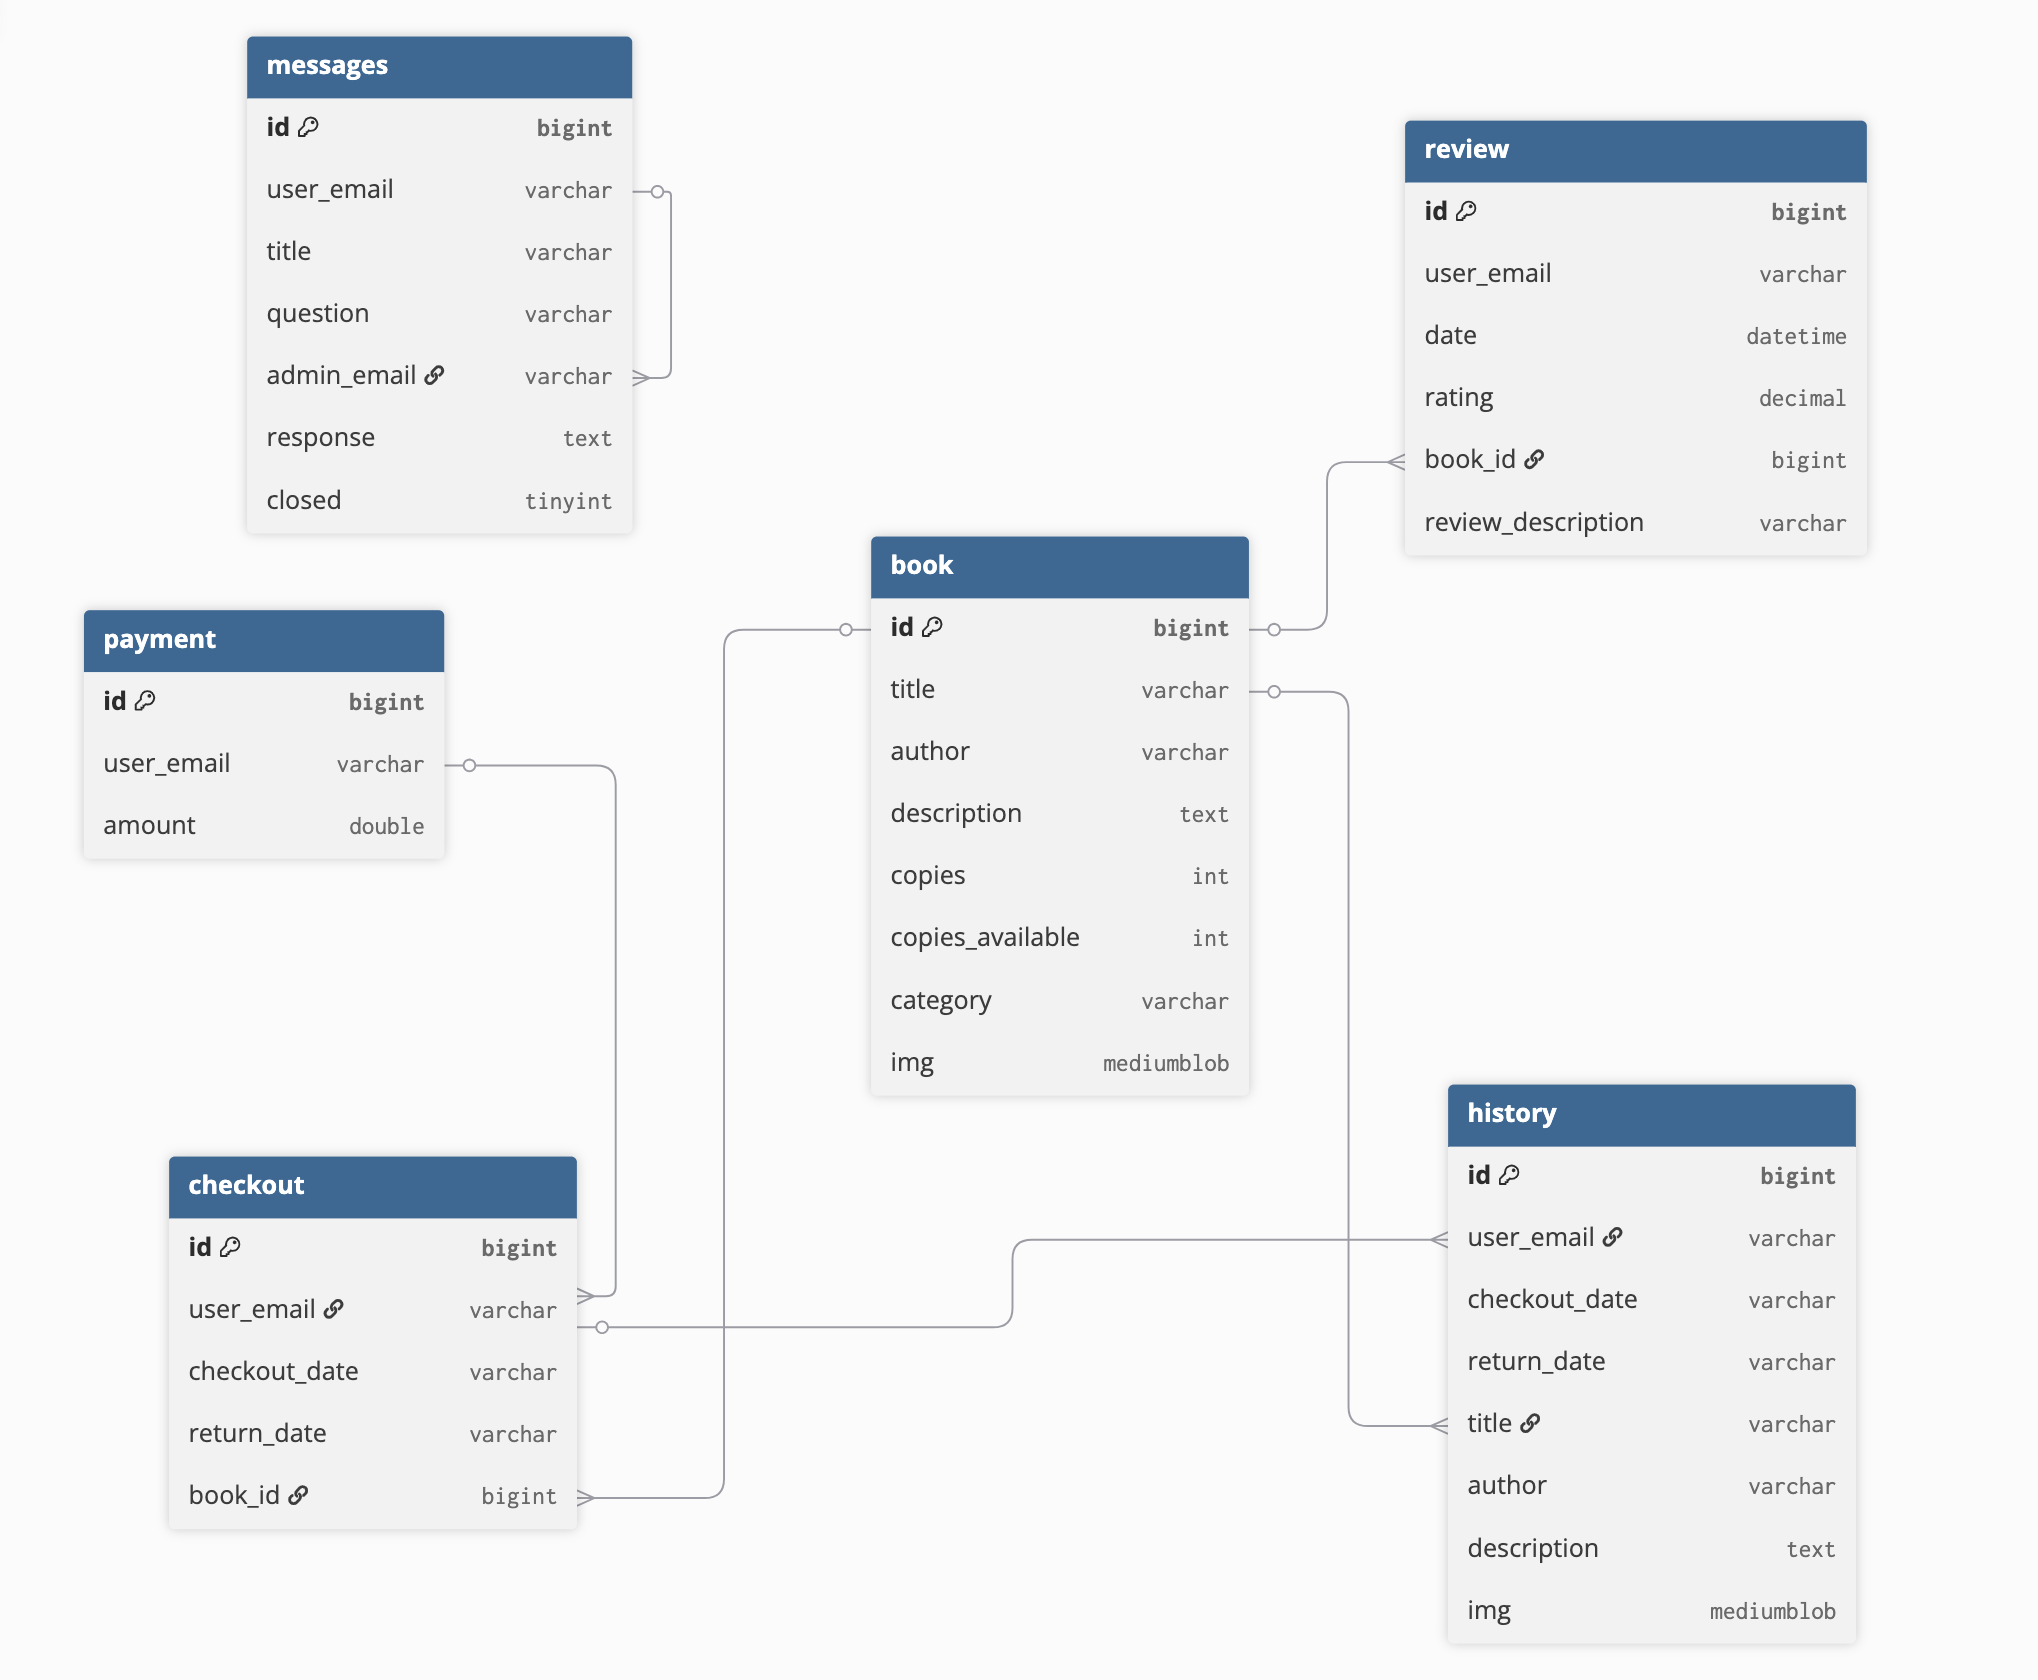
\includegraphics[width=0.99\textwidth]{images/DB-Schema.png}
	\caption{ER-Modell der Datenbank}
	\label{fig:er-model}
\end{figure}

\noindent Die logischen Beziehungen zwischen den Tabellen lassen sich wie folgt beschreiben:

\begin{itemize}
	\item Jede \texttt{checkout}-Instanz referenziert genau ein Buch über \texttt{book\_id}.
	\item Jede \texttt{review} ist einem Buch (book\_id) und einem Benutzer (user\_email) zugeordnet.
	\item Eine \texttt{message} verknüpft einen Benutzer mit einem Administrator über die jeweiligen E-Mail-Adressen.
	\item Ein \texttt{history}-Eintrag entspricht einer früheren Ausleihe eines Benutzers und speichert redundante Buchdaten.
	\item \texttt{payment}-Einträge entstehen nur bei verspäteter Rückgabe und sind über die Benutzer-E-Mail mit der Ausleihe verknüpft.
\end{itemize}


\subsection{Datenpersistenz mit Spring Data und Hibernate}\index{Datenpersistenz mit Spring Data und Hibernate}

Die Datenpersistenz wird mit Spring Boot in Verbindung mit Hibernate und Spring Data umgesetzt. Die Entitäten werden über Annotationen wie \texttt{@Entity}, \texttt{@Table}, \texttt{@Column}, \texttt{@Id}, und Beziehungen wie \texttt{@OneToMany} definiert.

\noindent Spring Data JPA und Spring Data REST übernehmen automatisch die Abbildung der Entitäten auf die Datenbanktabellen sowie die Bereitstellung von REST-APIs.

\noindent \textbf{Beispiel}: Entity-Klasse für Payments
\begin{lstlisting}[language=Java, caption={JPA-Entity \texttt{Payment}}, label={lst:Payment-entity}]
@Entity
@Table(name = "payment")
@Data
public class Payment {
	
	@Id
	@GeneratedValue(strategy = GenerationType.IDENTITY)
	private Long id;
	
	@Column(name = "user_email")
	private String userEmail;
	
	@Column(name = "amount")
	private double amount;
}
\end{lstlisting}

\noindent Diese Klasse stellt ein einfaches Beispiel für eine \texttt{Entity} dar, wie sie in Spring Data JPA und Hibernate verwendet wird. Die Annotationen übernehmen die automatische Zuordnung der Klasse zu einer Datenbanktabelle und ermöglichen eine saubere Trennung zwischen Domänenlogik und Datenpersistenz. Hier eine kurze Erklärung der wichtigsten Komponenten:

\begin{itemize}
	\item \texttt{@Entity}: Markiert die Klasse als JPA-Entity. Hibernate erkennt sie dadurch als persistente Klasse, die einer Tabelle in der Datenbank entspricht.
	
	\item \texttt{@Table(name = "payment")}: Gibt explizit an, dass die Klasse mit der Datenbanktabelle \texttt{payment} verknüpft ist. Falls die Annotation fehlt, würde standardmäßig der Klassenname als Tabellenname verwendet werden.
	
	\item \texttt{@Id}: Definiert das Feld \texttt{id} als Primärschlüssel der Tabelle.
	
	\item \texttt{@GeneratedValue(strategy = GenerationType.IDENTITY)}: Legt fest, dass der Primärschlüssel von der Datenbank automatisch (z.\,B.\ mittels AUTO\_INCREMENT) generiert wird. Dies ist typisch für MySQL.
	
	\item \texttt{@Column(name = "...")}: Weist jedes Attribut explizit einer Spalte in der Tabelle zu. Das ist besonders nützlich, wenn sich Feld- und Spaltennamen unterscheiden (z.\,B.\ \texttt{userEmail} $\rightarrow$ \texttt{user\_email}).
	
	\item \texttt{@Data} (aus Lombok): Generiert automatisch Getter, Setter, \texttt{equals()}, \texttt{hashCode()} und \texttt{toString()}-Methoden, um Boilerplate-Code zu vermeiden. Dies erhöht die Lesbarkeit und spart Entwicklungszeit.
\end{itemize}

\noindent \textbf{Beispiel}: Automatische Repository-Methoden mit Spring Data JPA and rest
\begin{lstlisting}[language=Java, caption={Payments-Repository-Schnittstelle}, label={lst:Payment-repo}]
public interface PaymentRepository extends JpaRepository<Payment, Long> {
	    Payment findByUserEmail(String userEmail);
}

\end{lstlisting}

\noindent Dieses Interface definiert die Datenzugriffsschicht für die \texttt{Payment}-Entität. Durch die Erweiterung von \texttt{JpaRepository<Payment, Long>} stellt Spring automatisch alle grundlegenden CRUD-Operationen bereit. \texttt{Payment} bezeichnet die Entitätsklasse, \texttt{Long} ist der Datentyp des Primärschlüssels.

\noindent Die Methode \texttt{findByUserEmail(String userEmail)} nutzt die Konventionen von Spring Data JPA: Anhand des Methodennamens erkennt Spring automatisch, dass nach dem Attribut \texttt{userEmail} gesucht werden soll, und generiert im Hintergrund die entsprechende SQL-Abfrage.

\noindent Da Spring Data REST als Abhängigkeit eingebunden ist, werden automatisch REST-Endpunkte für das Repository verfügbar gemacht – ohne dass man eigene Controller oder Services definieren muss. Die Endpunkte folgen dabei einer standardisierten Struktur:

\begin{itemize}
	\item \texttt{GET /payments} → Alle Zahlungen abrufen
	\item \texttt{POST /payments} → Neue Zahlung erstellen
	\item \texttt{GET /payments/1} → Zahlung mit ID 1 abrufen
	\item \texttt{DELETE /payments/1} → Zahlung mit ID 1 löschen
\end{itemize}

\noindent So ermöglichen Spring Data JPA und Spring Data REST gemeinsam eine saubere Trennung von Datenmodell und Zugriffsschicht – bei minimalem Implementierungsaufwand.


 
\chapter{Implementierung}

Im Rahmen dieses Kapitels wird exemplarisch eine der wichtigsten Funktionalitäten der Webanwendung behandelt – der Ausleihprozess sowie das Verfahren zur Rückgabe eines Buches.

\section{Ausleihprozess eines Buches}\index{Ausleihprozess eines Buches}
Im Folgenden wird der Ausleihprozess eines Buches aus Sicht des Backends sowie des Frontends detailliert beschrieben.

\subsection{Backend-Prozess}\index{Backend-Prozess}
In diesem Abschnitt wird der gesamte Backend-Prozess der Buchausleihe detailliert beschrieben. Die folgende Darstellung umfasst die beteiligten Repositories, die Service-Schicht inklusive aller Hilfsmethoden sowie den REST-Endpunkt im Controller.

\subsection*{Zugriff auf Daten: Repositories}

\textbf{1. \texttt{PaymentRepository}} \\
Da das \texttt{PaymentRepository} bereits im vorherigen Kapitel (siehe Listing~\ref{lst:Payment-repo}) im Zusammenhang mit Spring Data REST und JPA vorgestellt wurde, wird an dieser Stelle lediglich darauf verwiesen. Es wird für die Überprüfung offener Zahlungen verwendet.

\noindent \textbf{2. \texttt{CheckoutRepository}} \\
Für den Ausleihprozess wurde in diesem Repository (siehe Listing~\ref{lst:Checkout-repo}) diese Methoden genutzt:
\begin{lstlisting}[language=Java, caption=CheckoutRepository.java, label=lst:Checkout-repo, breaklines=true]
	public interface CheckoutRepository extends JpaRepository<Checkout, Long> {
		List<Checkout> findByUserEmail(String userEmail);
		Checkout findByBookIdAndUserEmail(Long bookId, String userEmail);
	}
\end{lstlisting}

\noindent Die erste Methode ruft alle ausgeliehenen Bücher eines bestimmten Nutzers anhand seiner E-Mail-Adresse ab. Die zweite Methode ruft einen einzelnen Checkout-Eintrag aus der Datenbank ab, der zur angegebenen E-Mail-Adresse des Benutzers und der ID des Buches gehört.

\subsection*{Geschäftslogik: Die Methode \texttt{checkoutBook} im BookService}

Die Methode \texttt{checkoutBook} (siehe Listing~\ref{lst:Checkout-service}) enthält den gesamten Ablauf der Buchausleihe. Im Folgenden wird die Methode vollständig dargestellt und im Anschluss schrittweise erklärt:

\begin{lstlisting}[style=pseudocode, caption=checkoutBook() Methode im BookService.java, label=lst:Checkout-service]
	public Book checkoutBook(String userEmail, Long bookId) throws Exception {
		Book book = bookRepository.findById(bookId)
		.orElseThrow(() -> new BookNotAvailableException("Book with ID " + bookId + " is not available."));
		
		checkAvailability(book, userEmail);
		
		List<Checkout> userCheckouts = checkoutRepository.findByUserEmail(userEmail);
		boolean hasOverdueBooks = hasOverdueBooks(userCheckouts);
		
		Payment payment = paymentRepository.findByUserEmail(userEmail);
		
		if ((payment != null && payment.getAmount() > 0) || (payment != null && hasOverdueBooks)) {
			throw new Exception("The loan has been blocked due to outstanding payments or overdue books.");
		}
		
		if (payment == null) {
			createZeroPayment(userEmail);
		}
		
		decrementBookStock(book);
		createCheckoutRecord(userEmail, book);
		
		return book;
	}
\end{lstlisting}

\noindent \textbf{Erklärung:}\\
- \textbf{Zeile 2--3:} Das Buch wird anhand der ID geladen. Wenn es nicht existiert, wird eine Ausnahme geworfen. \\
- \textbf{Zeile 5:} Es wird geprüft, ob das Buch verfügbar ist und noch nicht vom Benutzer ausgeliehen wurde. \\
- \textbf{Zeile 7:} Alle bisherigen Ausleihen des Benutzers werden geladen. \\
- \textbf{Zeile 8:} Es wird überprüft, ob überfällige Bücher dabei sind.\\
- \textbf{Zeile 10:} Die Zahlungsinformationen des Benutzers werden geladen.\\
- \textbf{Zeile 12--14:} Falls offene Zahlungen oder überfällige Bücher vorhanden sind, wird eine Sperre ausgelöst.\\
- \textbf{Zeile 16--18:} Wenn kein Zahlungseintrag vorhanden ist, wird einer mit 0 Euro erstellt.\\
- \textbf{Zeile 20:} Der Buchbestand wird um eins reduziert.\\
- \textbf{Zeile 21:} Ein neuer Ausleihdatensatz wird erstellt.\\
- \textbf{Zeile 23:} Das Buchobjekt wird zurückgegeben.\\

\noindent \textbf{Hilfsmethoden:}
\begin{lstlisting}[style=pseudocode, caption=Überprüfung der Verfügbarkeit eines Buches, label=checkAvailability]
	private void checkAvailability(Book book, String userEmail) {
	if (checkoutRepository.findByBookIdAndUserEmail(book.getId(), userEmail) != null) {
			throw new BookNotAvailableException("The book has already been borrowed.");
		}
		if (book.getCopiesInStock() <= 0) {
			throw new BookNotAvailableException("No copies available for loan.");
		}
	}
\end{lstlisting}
Diese Methode \ref{checkAvailability} überprüft, ob das angegebene Buch bereits von dem betreffenden Benutzer ausgeliehen wurde. Falls dies zutrifft, wird eine entsprechende Ausnahme ausgelöst, um eine doppelte Ausleihe zu verhindern. Zusätzlich wird geprüft, ob noch verfügbare Exemplare des Buches vorhanden sind. Ist dies nicht der Fall, wird ebenfalls eine Ausnahme ausgelöst, sodass keine Ausleihe ohne Bestand erfolgen kann.

\begin{lstlisting}[language=Java, caption=Prüfung auf überfällige Ausleihen, label=lst:hasOverdueBooks]
	private boolean hasOverdueBooks(List<Checkout> checkouts) {
		LocalDate today = LocalDate.now();
		
		for (Checkout checkout : checkouts) {
			LocalDate returnDate = LocalDate.parse(checkout.getReturnedAt());
			if (returnDate.isBefore(today)) {
				return true;
			}
		}
		return false;
	}
\end{lstlisting}
Diese Methode  \ref{lst:hasOverdueBooks} überprüft, ob in der übergebenen Liste von Checkout-Einträgen mindestens ein Buch enthalten ist, dessen Rückgabedatum vor dem heutigen Datum liegt – also überfällig ist.

\begin{lstlisting}[language=Java, caption=Erstellung einer Nullzahlung mit createZeroPayment(), label=createZeroPayment]
	private void createZeroPayment(String userEmail) {
		Payment newPayment = Payment.builder()
		         .userEmail(userEmail)
		         .amount(0.0)
		         .build();
		paymentRepository.save(newPayment);
	}
\end{lstlisting}
Diese Methode \ref{createZeroPayment} erstellt einen neuen Zahlungseintrag mit dem Betrag 0.0 für die angegebene Benutzer-E-Mail und speichert sie in der Datenbank über das PaymentRepository.

\begin{lstlisting}[language=Java, caption=Reduzierung des Buchbestands, label=decrementBookStock]
	private void decrementBookStock(Book book) {
		book.setCopiesInStock(book.getCopiesInStock() - 1);
		bookRepository.save(book);
	}
\end{lstlisting}
Diese Methode \ref{decrementBookStock} reduziert den Lagerbestand des übergebenen Buchs um eins und speichert die Änderung in der Datenbank.

\begin{lstlisting}[language=Java, caption=Erstellung eines Ausleihdatensatzes, label=createCheckoutRecord, breaklines=true]
	private void createCheckoutRecord(String userEmail, Book book) {
		Checkout checkout = new Checkout(userEmail, LocalDate.now().toString(),
		LocalDate.now().plusDays(CHECKOUT_PERIOD_DAYS).toString(), book.getId());
		checkoutRepository.save(checkout);
	}
\end{lstlisting}
Diese Methode \ref{createCheckoutRecord} erstellt einen neuen Ausleihdatensatz für das angegebene Buch und den Benutzer mit dem aktuellen Datum und speichert ihn in der Datenbank.


\subsection*{Schnittstelle zum Frontend: BookController}

Der REST-Endpunkt (siehe \ref{BookController.java}) empfängt Anfragen zur Ausleihe und leitet sie an den Service weiter:

\begin{lstlisting}[language=Java, caption=REST-Endpunkt \texttt{checkoutBook()} im \texttt{BookController}, label=BookController.java]
	@PutMapping("/secure/loans/checkout")
	public Book checkoutBook(Authentication authentication,
	@RequestParam Long bookId) throws Exception {
		String userEmail = authentication.getName();
		return bookService.checkoutBook(userEmail, bookId);
	}
\end{lstlisting}

\noindent - \texttt{@PutMapping}: Definiert den Pfad zum Ausleih-Endpunkt.\\
- \texttt{Authentication}: Ermöglicht Zugriff auf die Benutzerinformationen über Spring Security.\\
- Die Methode ruft den Ausleihprozess im Service auf und gibt das ausgeliehene Buch zurück.

\subsection{Frontend-Prozess}\index{Frontend-Prozess}

Im Frontend wird der Ausleihprozess in der Komponente \texttt{CheckoutBook} umgesetzt. Hierzu werden die Methode \texttt{checkoutBook()} für den API-Aufruf und die Konstante \texttt{checkoutButton} zur Darstellung der passenden Benutzeroberfläche verwendet.

\subsection*{API-Aufruf zur Ausleihe eines Buches}

Die folgende Methode (siehe \ref{checkoutBook.tsx}) übernimmt den API-Aufruf an das Backend, um ein Buch auszuleihen:

\begin{lstlisting}[language=Java, caption=Implementierung der checkoutBook()-Funktion in CheckoutBook.tsx, label=checkoutBook.tsx, breaklines=true]
	async function checkoutBook() {
		const apiUrl = `${process.env.REACT_APP_API_URL}/books/secure/loans/checkout?bookId=${bookId}`;
		const response = {
			method: 'PUT',
			headers: {
				Authorization: `Bearer ${authState?.accessToken?.accessToken}`,
				'Content-Type': 'application/json'
			}
		};
		const res = await fetch(apiUrl, response);
		if (!res.ok) {
			setShowError(true);
			return;
		}
		setShowError(false);
		setIsBookCheckedOut(true);
	}
\end{lstlisting}

\noindent \textbf{Erklärung:}\\
- \texttt{apiUrl}: Baut die URL für den API-Endpunkt mit dem Buch-ID als Parameter.\\
- \texttt{response}: Enthält die Methode (PUT) und den Authentifizierungs-Token.\\
- \texttt{fetch()}: Sendet die Anfrage an das Backend.\\
- \texttt{!res.ok}: Falls der Server einen Fehler zurückgibt, wird ein Fehler angezeigt.\\
- \texttt{setShowError(false)}: Versteckt die Fehlermeldung, falls alles korrekt lief.\\
- \texttt{setIsBookCheckedOut(true)}: Setzt den Status, dass das Buch nun ausgeliehen ist.

\subsection*{Benutzeroberfläche: Auswahl der richtigen Aktion}

Die Konstante \texttt{checkoutButton} (siehe Listing~\ref{renderButton()}) bestimmt dynamisch, welcher Button oder welche Nachricht dem Benutzer im Ausleihbereich angezeigt wird. 

\begin{itemize}
	\item \textbf{Zeilen 1--2:} \texttt{useMemo(() => \{ ... \}, [...])} stellt sicher, dass die Berechnung des Buttons nur dann neu ausgeführt wird, wenn sich die abhängigen Werte ändern (\texttt{props.isAuthenticated}, \texttt{props.isCheckedOut}, \texttt{props.currentLoans}, \texttt{props.checkoutBook}, \texttt{t}).
	\item \textbf{Zeilen 3--8:} Wenn der Benutzer nicht authentifiziert ist (\texttt{!props.isAuthenticated}), wird ein \texttt{Link}-Element zur Login-Seite zurückgegeben, das den Text \textbf{Anmelden} anzeigt.
	\item \textbf{Zeilen 10--31:} Wenn das Buch noch nicht ausgeliehen wurde (\texttt{!props.isCheckedOut}) und der Benutzer noch weniger als 5 Bücher ausgeliehen hat (\texttt{props.currentLoans < 5}):
	\begin{itemize}
		\item \textbf{Zeilen 12--20:} Überprüft, ob keine Exemplare verfügbar sind (\texttt{!props.book?.copiesInStock || props.book.copiesInStock <= 0}). Ist dies der Fall, wird ein deaktivierter Button angezeigt.
		\item \textbf{Zeilen 22--31:} Andernfalls wird ein aktiver Checkout-Button zurückgegeben, der beim Klicken die Methode \texttt{props.checkoutBook()} ausführt. Der Button zeigt ebenfalls \textbf{Ausleihen} an.
	\end{itemize}
	\item \textbf{Zeilen 33--40:} Wenn das Buch bereits ausgeliehen ist (\texttt{props.isCheckedOut}), wird eine Erfolgsnachricht in einem \texttt{<p>}-Element angezeigt, inklusive eines grünen Häkchen-Icons und des Textes \textbf{Bereits ausgeliehen}.
	\item \textbf{Zeilen 42--47:} In allen anderen Fällen, z.\,B. wenn der Benutzer die maximale Anzahl an Ausleihen erreicht hat, wird eine Warnmeldung in einem \texttt{<p>}-Element mit rotem Icon und dem Text \textbf{Die maximale Anzahl an Checkouts wurde erreicht} angezeigt.
	\item \textbf{Zeilen 49--54:} Die Werte \texttt{props.isAuthenticated}, \texttt{props.isCheckedOut}, \texttt{props.currentLoans}, \texttt{props.checkoutBook} und \texttt{t} werden als Abhängigkeiten übergeben, sodass die Berechnung des Buttons nur erneut erfolgt, wenn sich einer dieser Werte ändert. Sie repräsentieren den Authentifizierungsstatus, den Ausleihstatus des Buches, die Anzahl der aktuellen Ausleihen, die Funktion zum Ausleihen eines Buches sowie die Übersetzungsfunktion.
\end{itemize}

\noindent Auf diese Weise sorgt \texttt{checkoutButton} dafür, dass die Benutzeroberfläche stets den aktuellen Status des Benutzers und des Buches korrekt darstellt, während \texttt{useMemo} unnötige Neuberechnungen verhindert und die Performance optimiert.
\subsection*{Einbindung des Buttons in die Oberfläche}

\noindent Dieses \texttt{checkoutButton}-Konstantenobjekt wird anschließend innerhalb des \texttt{return()}-Statements aufgerufen,  als \{\texttt{checkoutButton}\}, innerhalb der Datei \texttt{ReviewCheckoutPanel.tsx}.


\section{Verfahren zur Rückgabe eines Buches}\index{Verfahren zur Rückgabe eines Buches}
Im Folgenden wird das Verfahren zur Rückgabe eines Buches sowohl im Backend als auch im Frontend erläutert.

\subsection{Backend-Prozess}\index{Backend-Prozess}
Der Rückgabeprozess nutzt die bereits beschriebenen Repositories \ref{lst:Checkout-repo} und \ref{lst:Payment-repo}. 

\subsection*{Geschäftslogik: Die Methode \texttt{returnBook} im BookService.java} 

Die wesentliche Logik für die Rückgabe eines Buches ist in der Methode \texttt{returnBook} der Datei \texttt{BookService.java} implementiert (siehe Listing~\ref{returnBook().java}).

\noindent \textbf{Erklärung:}

\begin{itemize}
	\item \textbf{Zeilen 1--3:}  
	Das Buch mit der angegebenen \texttt{bookId} wird aus der Datenbank abgerufen. Existiert das Buch nicht, wird eine Ausnahme ausgelöst, die signalisiert, dass das Buch nicht verfügbar ist.
	
	\item \textbf{Zeilen 5--8:}  
	Es wird nach einem aktiven Ausleihdatensatz (\texttt{Checkout}) für dieses Buch und diesen Benutzer gesucht. Falls kein Eintrag gefunden wird, wird eine Ausnahme ausgelöst, um eine ungültige Rückgabe zu verhindern.
	
	\item \textbf{Zeilen 10--11:}  
	Der Lagerbestand des Buchs wird um eins erhöht und die geänderte Buch-Entität in der Datenbank gespeichert.
	
	\item \textbf{Zeilen 13--15:}  
	Das Rückgabedatum des Ausleihdatensatzes wird geparst, das aktuelle Datum ermittelt und die Anzahl der überfälligen Tage berechnet.
	
	\item \textbf{Zeilen 17--28:}  
	Wenn das Buch überfällig ist, wird der Zahlungsdatensatz des Benutzers abgerufen. Existiert kein Eintrag, wird ein neuer Zahlungsdatensatz mit 0.0 erstellt. Der Betrag wird basierend auf den überfälligen Tagen (2 Einheiten pro Tag) aktualisiert und gespeichert.
	
	\item \textbf{Zeile 30:}  
	Der Ausleihdatensatz wird aus der Datenbank gelöscht, wodurch das Buch offiziell als zurückgegeben markiert wird.
	
	\item \textbf{Zeilen 32--42 (Historie erfassen):}  
	Ein Historieneintrag für diese Ausleihe wird erstellt, einschließlich Buchinformationen, Ausleihdatum und Rückgabedatum. Dieser Eintrag wird gespeichert, um eine dauerhafte Aufzeichnung der Transaktion zu gewährleisten.
\end{itemize}



\subsection*{Rückgabe-Endpunkt im Controller}

Die Controller-Methode(siehe  \ref{lst:returnBook()}) ist für die Entgegennahme der Anfrage aus dem Frontend zuständig:

\begin{lstlisting}[language=Java, caption=returnBook() Endpoint in BookController.java, label=lst:returnBook()]
	@PutMapping("/secure/loans/return")
	public void returnBook(Authentication authentication,
	@RequestParam Long bookId) throws ParseException {
		String userEmail = authentication.getName();
		bookService.returnBook(userEmail, bookId);
	}
\end{lstlisting}

\noindent \textbf{Erklärung:}\\
- Der Endpunkt verarbeitet eine PUT-Anfrage mit dem Buch-ID als Parameter.\\
- Die E-Mail des Benutzers wird über das Authentication-Objekt extrahiert.\\
- Der Service übernimmt die Logik für die Rückgabe.

\subsection{Frontend-Prozess}\index{Frontend-Prozess}
Die Rückgabe eines Buches erfolgt durch einen Button innerhalb der Benutzeroberfläche  der ausgeliehenen Bücher. Der Button ist wie folgt definiert (siehe \ref{retrurnBook-Button}):

\begin{lstlisting}[style=pseudocode, caption=retrurnBook-Button in LoanDetailsModal.tsx, label=retrurnBook-Button]
	<button
	onClick={() => props.returnBook(props.userLoanSummary.book.id)}
	type="button"
	data-bs-dismiss="modal"
	className="btn btn-outline-success rounded-pill py-1 px-2 mb-2 small"
	>
	{t("loanDetails.returnBook")}
	</button>
\end{lstlisting}

\noindent \textbf{Erklärung:}
\begin{itemize}
	\item \texttt{onClick={() => props.returnBook(props.userLoanSummary.book.id)}}: Beim Klick wird die Funktion \texttt{returnBook()} mit der \texttt{bookId} des ausgeliehenen Buches aufgerufen.
	\item \texttt{data-bs-dismiss="modal"}: Schließt das Bootstrap-Modal nach dem Klick automatisch.
	\item \texttt{className="..."}: Definiert das Styling des Buttons (grün, umrandet, abgerundet, klein).
	\item \texttt{{t("loanDetails.returnBook")}}: Holt den lokalisierten Text für „Buch zurückgeben“ aus der Übersetzungsdatei.
\end{itemize}

\noindent Beim Klicken auf den Button wird die Methode \texttt{returnBook()} (siehe \ref{returnBook-fucntion}) aufgerufen, welche als \texttt{async} Funktion in der Datei \texttt{loans.tsx} definiert ist:


\begin{lstlisting}[style=pseudocode, caption=returnBook() in Loans.tsx, label=returnBook-fucntion, breaklines=true]
	async function returnBook(bookId: number) {
		const apiUrl = `${process.env.REACT_APP_API_URL}/books/secure/loans/return?bookId=${bookId}`;
		const requestOptions = {
			method: 'PUT',
			headers: {
				Authorization: `Bearer ${authState?.accessToken?.accessToken}`,
				'Content-Type': 'application/json'
			}
		};
		const data = await fetch(apiUrl, requestOptions);
		if (!data.ok) {
			throw new Error('Something went wrong while returning the book!');
		}
		setCheckout(!checkout);
	}
\end{lstlisting}

\noindent \textbf{Erklärung:}
\begin{itemize}
	\item \texttt{const apiUrl = ...}: Erstellt die API-URL mit Query-Parameter \texttt{bookId}, um das Rückgabe-Ende im Backend anzusprechen.
	\item \texttt{const requestOptions = \{\}}: Konfiguriert die HTTP-Anfrage mit Methode und Headern.
	\item \texttt{method: 'PUT'}: Gibt an, dass es sich um eine \texttt{PUT}-Anfrage handelt (für Rückgabe geeignet).
	\item \texttt{Authorization: \texttt{Bearer ...}}: Hängt das JWT-Token im Header an, um die Anfrage zu authentifizieren.
	\item \texttt{'Content-Type': 'application/json'}: Gibt das Format der übertragenen Daten an.
	\item \texttt{const data = await fetch(...)}: Führt die Anfrage asynchron aus und wartet auf die Antwort.
	\item \texttt{if (!data.ok)}: Überprüft, ob ein Fehler vom Server zurückgegeben wurde.
	\item \texttt{throw new Error(...)}: Löst bei Fehlern eine Ausnahme mit passender Meldung aus.
	\item \texttt{setCheckout(!checkout)}: Aktualisiert den \texttt{checkout}-State, um die Oberfläche neu zu laden bzw. den Rückgabezustand zu reflektieren.
\end{itemize}

\chapter{Beispiel}
Dieses Kapitel bietet einen umfassenden Überblick über die Funktionalität und Benutzerfreundlichkeit der Anwendung. Anhand einer Reihe detaillierter Screenshots wird die Bedienung des Systems anschaulich dargestellt und analysiert. Dadurch erhalten die Leserinnen und Leser einen praxisnahen Einblick in den Umgang mit der Anwendung sowie die einzelnen Arbeitsschritte.

\section{Startseite}\index{Startseite}

Die Startseite der Anwendung dient als zentraler Einstiegspunkt für alle Nutzergruppen. Sie bietet einen Überblick über die wichtigsten Funktionen der App, wie die Buchsuche, aktuelle Empfehlungen und den Zugang zu weiterführenden Diensten. Die Benutzeroberfläche ist übersichtlich gestaltet und ermöglicht eine intuitive Navigation durch die verschiedenen Inhalte. In diesem Teil wird gezeigt, wie die Startseite strukturiert ist und welche interaktiven Elemente den Nutzerinnen und Nutzern zur Verfügung stehen.

\subsection{Header und Navigation}\index{Header und Navigation}
Die folgende Abbildung \ref{fig:header} zeigt den Aufbau des Headers mit dem dynamischen Navigationsmenü, das sich je nach Benutzerrolle unterscheidet:

\begin{figure}[H]
	\centering
	
\includegraphics[width=1.0\textwidth]{images/UI-screenshots/Header.png}
	\caption{ Kopfzeile der App \textit{Libranova}}
	\label{fig:header}
\end{figure}

\begin{itemize}
	\item \textbf{Besucher:} Anzeige des \textit{Libranova}-Logos sowie der Menüpunkte \textbf{Startseite} und \textbf{Bücher Suchen}. Rechts oben befindet sich ein \textbf{Login}-Button. Außerdem steht ein Dropdown-Menü zur Auswahl der Sprache (Deutsch oder Englisch) zur Verfügung.
	\item \textbf{Eingeloggte Nutzer:} Zusätzlich zu den Besucher-Menüpunkten sind \textbf{Bibliotheksaktivität} (Einblick in ausgeliehene Bücher und Ausleihhistorie) sowie \textbf{Überfällige Gebühren} (Anzeige möglicher Gebühren für verspätete Rückgaben) sichtbar. Rechts oben wird ein \textbf{Logout}-Button angezeigt. 
	\item \textbf{Administratoren:} Alle Menüpunkte der eingeloggten Nutzer plus der Menüpunkt \textbf{Admin}, welcher Verwaltungsfunktionen für den Buchbestand (Hinzufügen, Ändern, Löschen) und die Bearbeitung von Kundenanfragen umfasst.
\end{itemize}

\subsection{Footer}\index{Footer}
Die folgende Abbildung \ref{fig:footer} zeigt die Fußzeile der Anwendung. Sie enthält das Copyright \textcopyright\ Libranova App, Inc sowie die Menüpunkte \textbf{Startseite} und \textbf{Bücher suchen}.

\begin{figure}[H]
	\centering
	
\includegraphics[width=1.0\textwidth]{images/UI-screenshots/Footer.png}%\subsection{Startseite (Main Page)}
	\caption{ Kopfzeile der App \textit{Libranova}}
	\label{fig:footer}%\subsubsection{Karussell (Carousel)}
\end{figure}

\subsection{Hauptteil}\index{Hauptteil}

\subsection*{Karussell und Buch-Browser}\index{Karussell und Buch-Browser}

Die folgende Abbildung  \ref{fig:Carousel_and_BookBrowser} zeigt ein Karussell zur Darstellung ausgewählter Bücher sowie einen Button, der zur Suchseite für Bücher weiterleitet.

\begin{figure}[H]
	\centering
	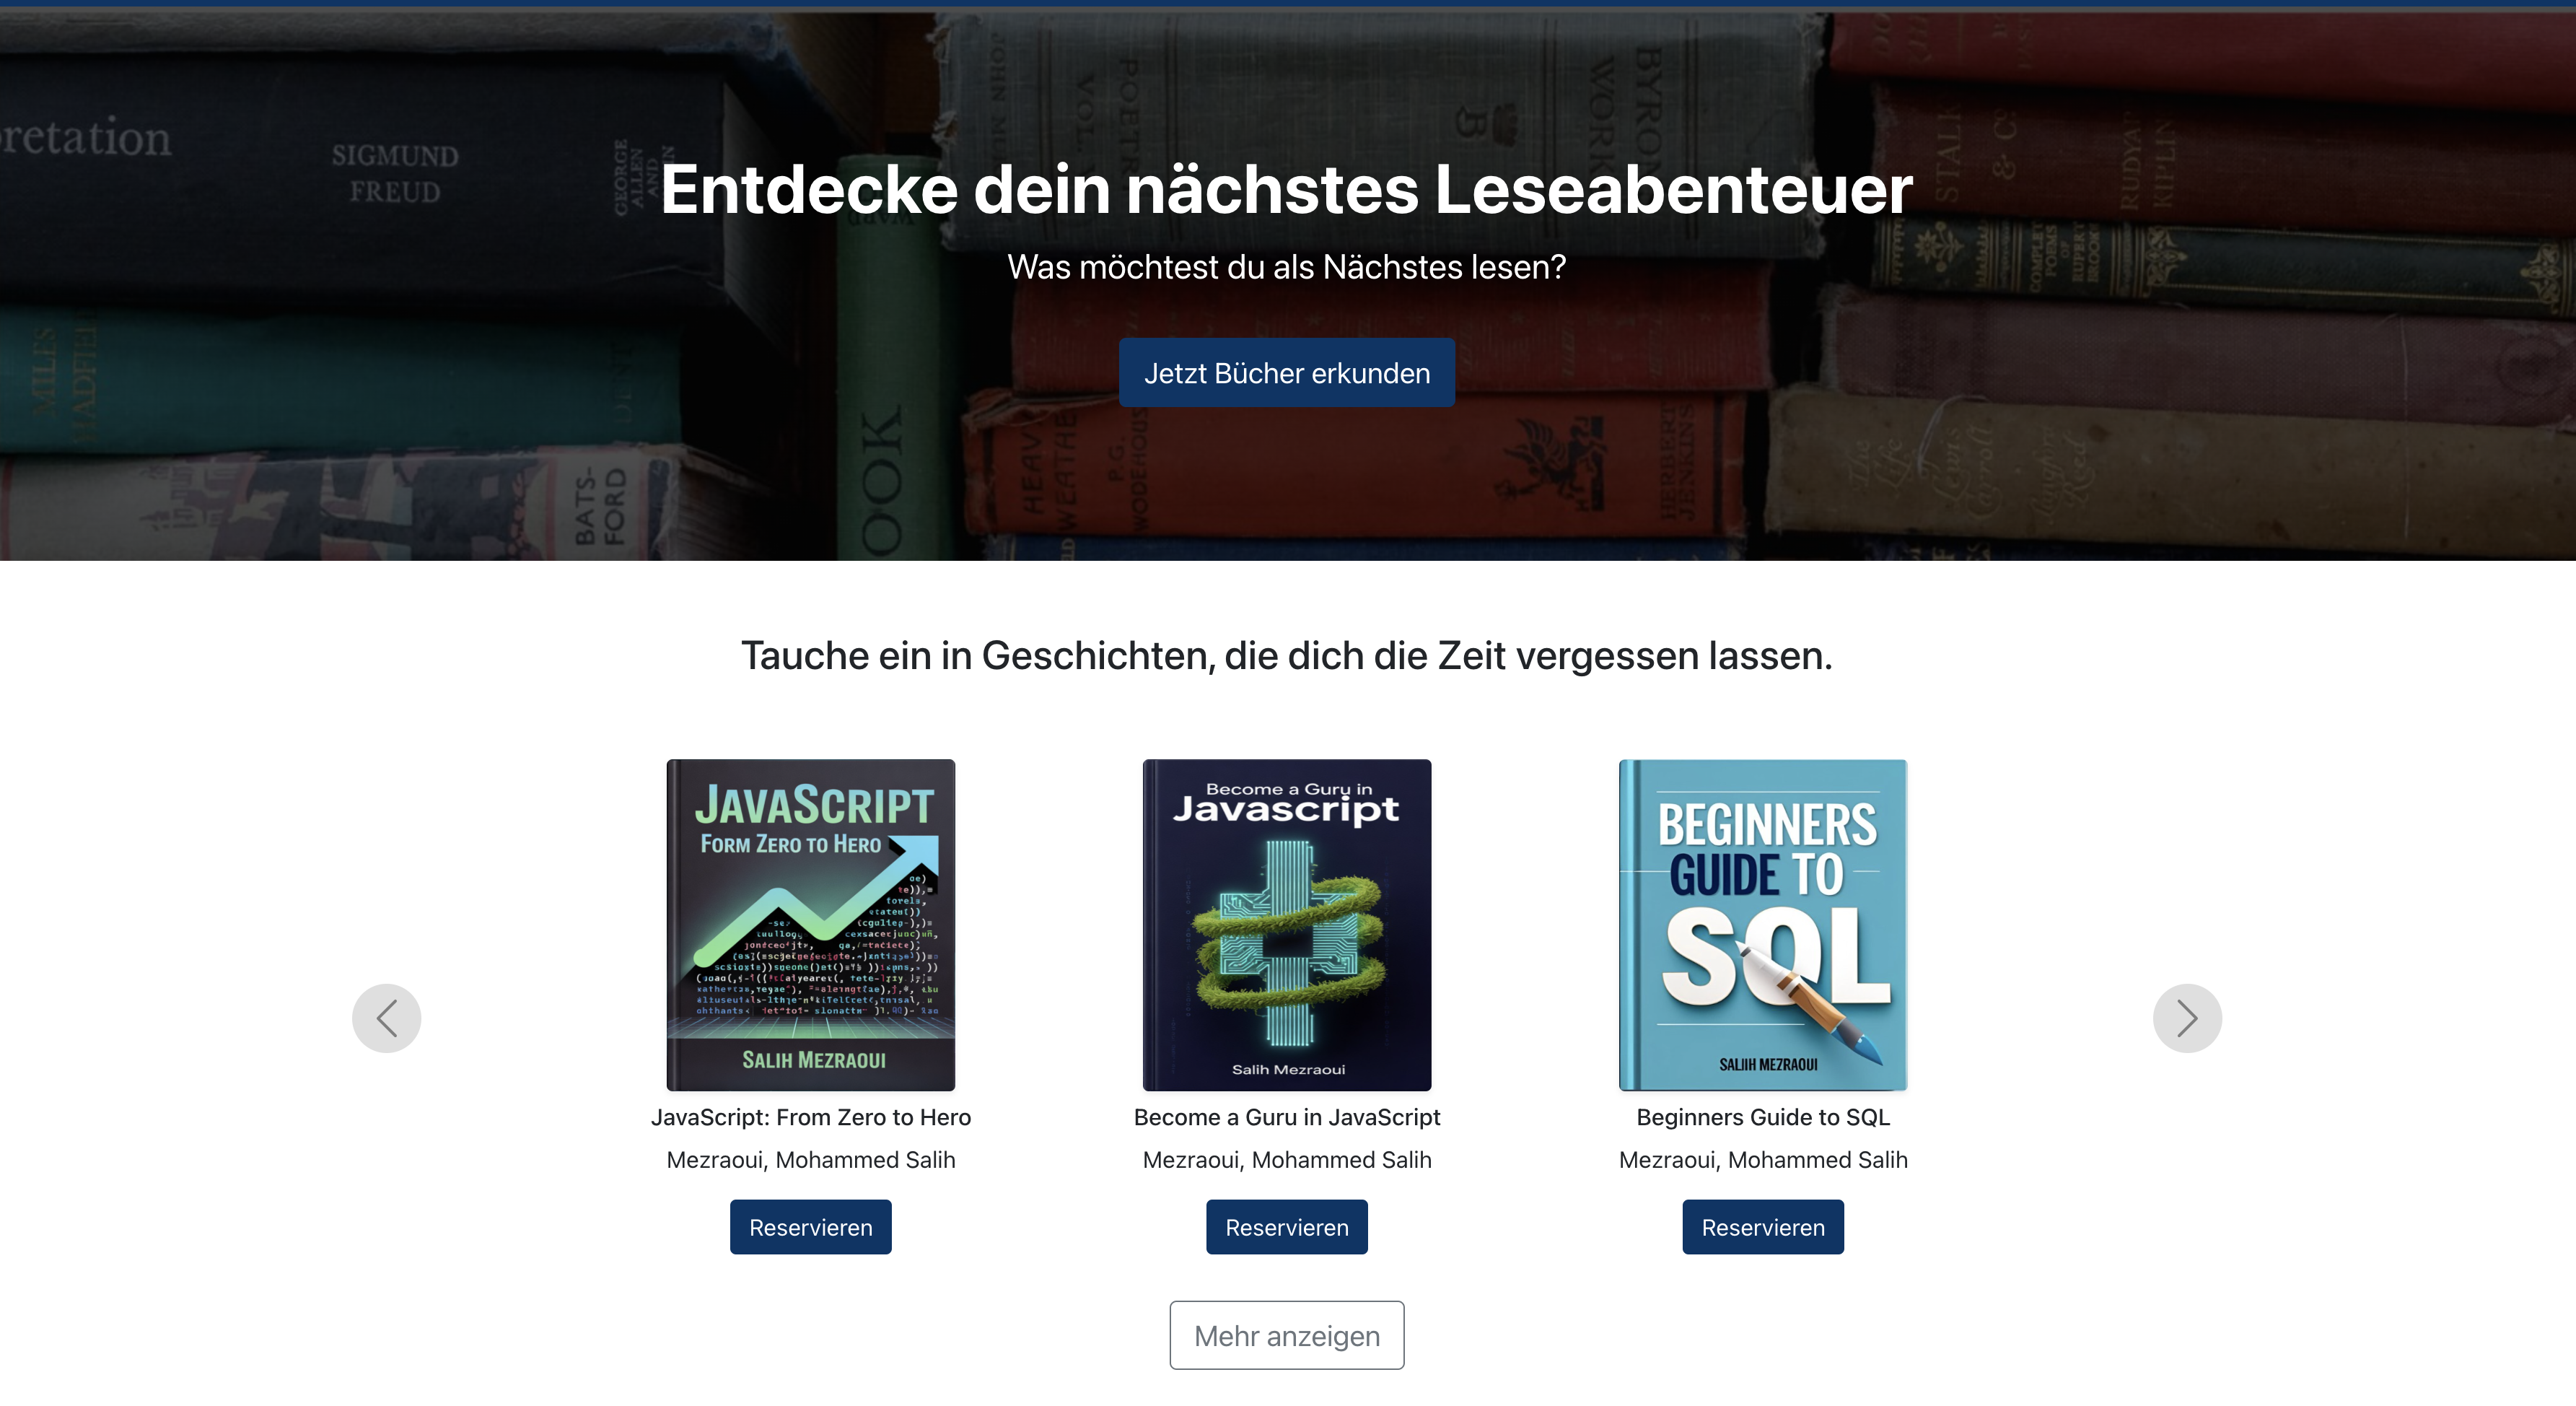
\includegraphics[width=1.0\textwidth]{images/UI-screenshots/Carousel_and_BookBrowser.png}%\subsection{Startseite (Main Page)}
	\caption{Karussell und Buch-Browser-Schaltfläche}
	\label{fig:Carousel_and_BookBrowser}%\subsubsection{Karussell (Carousel)}
\end{figure}

\subsection*{}\index{Link zur Bibliotheksdienste}

Die folgende Abbildung \ref{fig:Bibliotheksdienste-Link} zeigt einen Link zu den Bibliotheksdiensten, der angezeigt wird, wenn der Benutzer angemeldet ist. Andernfalls erscheint die Option ‚Registrieren‘.

\begin{figure}[H]
	\centering
	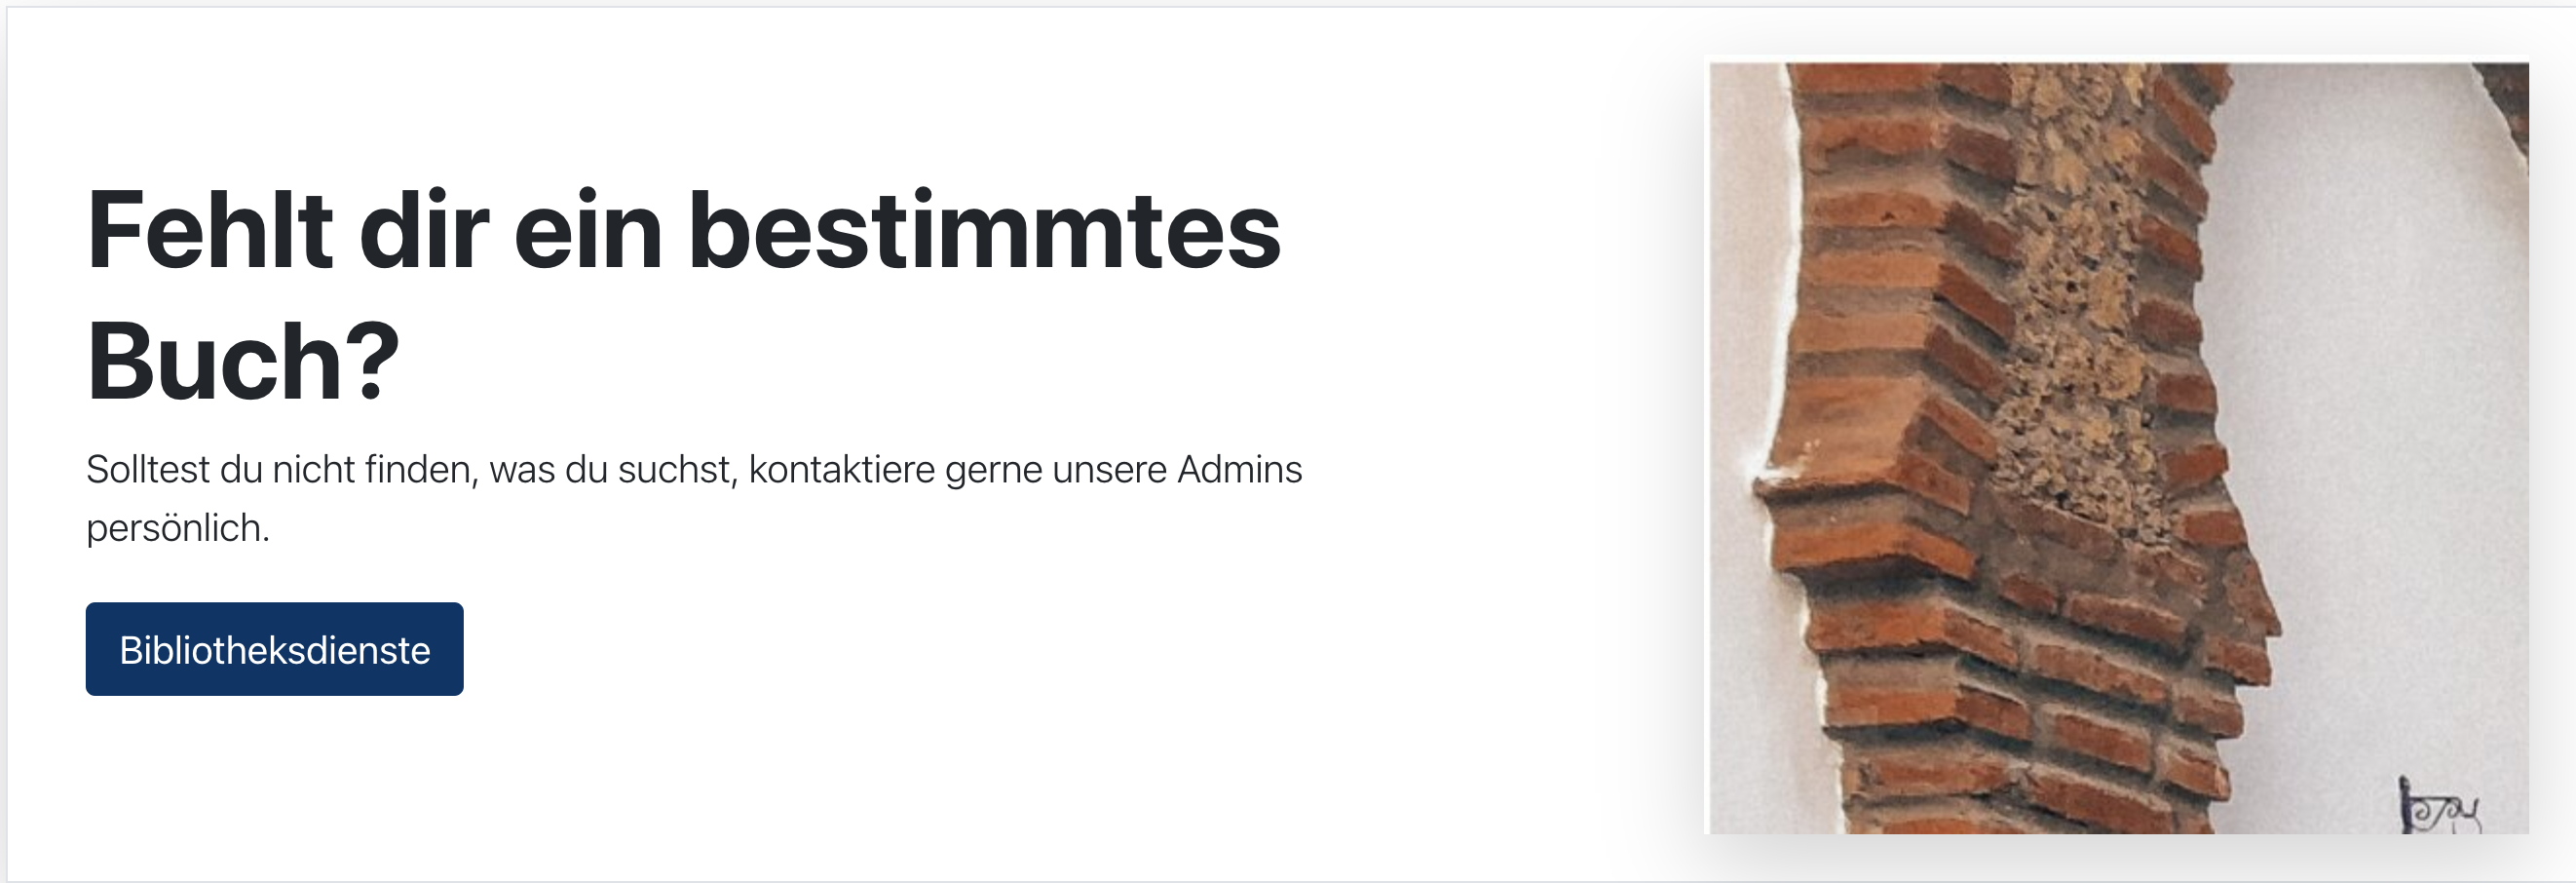
\includegraphics[width=1.0\textwidth]{images/UI-screenshots/Bibliotheksdienste-Link.png}%\subsection{Startseite (Main Page)}
	\caption{Karussell und Buch-Browser-Schaltfläche}
	\label{fig:Bibliotheksdienste-Link}%\subsubsection{Karussell (Carousel)}
\end{figure}

\section{Seitenübersicht}
Dieser Abschnitt gibt einen Überblick über zentrale Benutzeroberflächen der Anwendung, insbesondere die Buchsuchseite und die Buchdetailseite, und beschreibt deren wichtigste Funktionselemente.

\subsection{Buchsuche}

Die untenstehende Abbildung  \ref{fig:Search-page} zeigt die Benutzeroberfläche der Suchseite. Sie enthält ein Suchfeld mit Schaltfläche sowie ein Dropdown-Menü zur Auswahl von Kategorien. Nutzer können entweder nach Stichwörtern, Kategorien oder einer Kombination aus beiden suchen. Die Suchergebnisse werden in paginierter Form dargestellt und beinhalten jeweils den Buchtitel, den Autor, eine Kurzbeschreibung sowie eine Schaltfläche zur Detailansicht des jeweiligen Buches.

\begin{figure}[H]
	\centering
	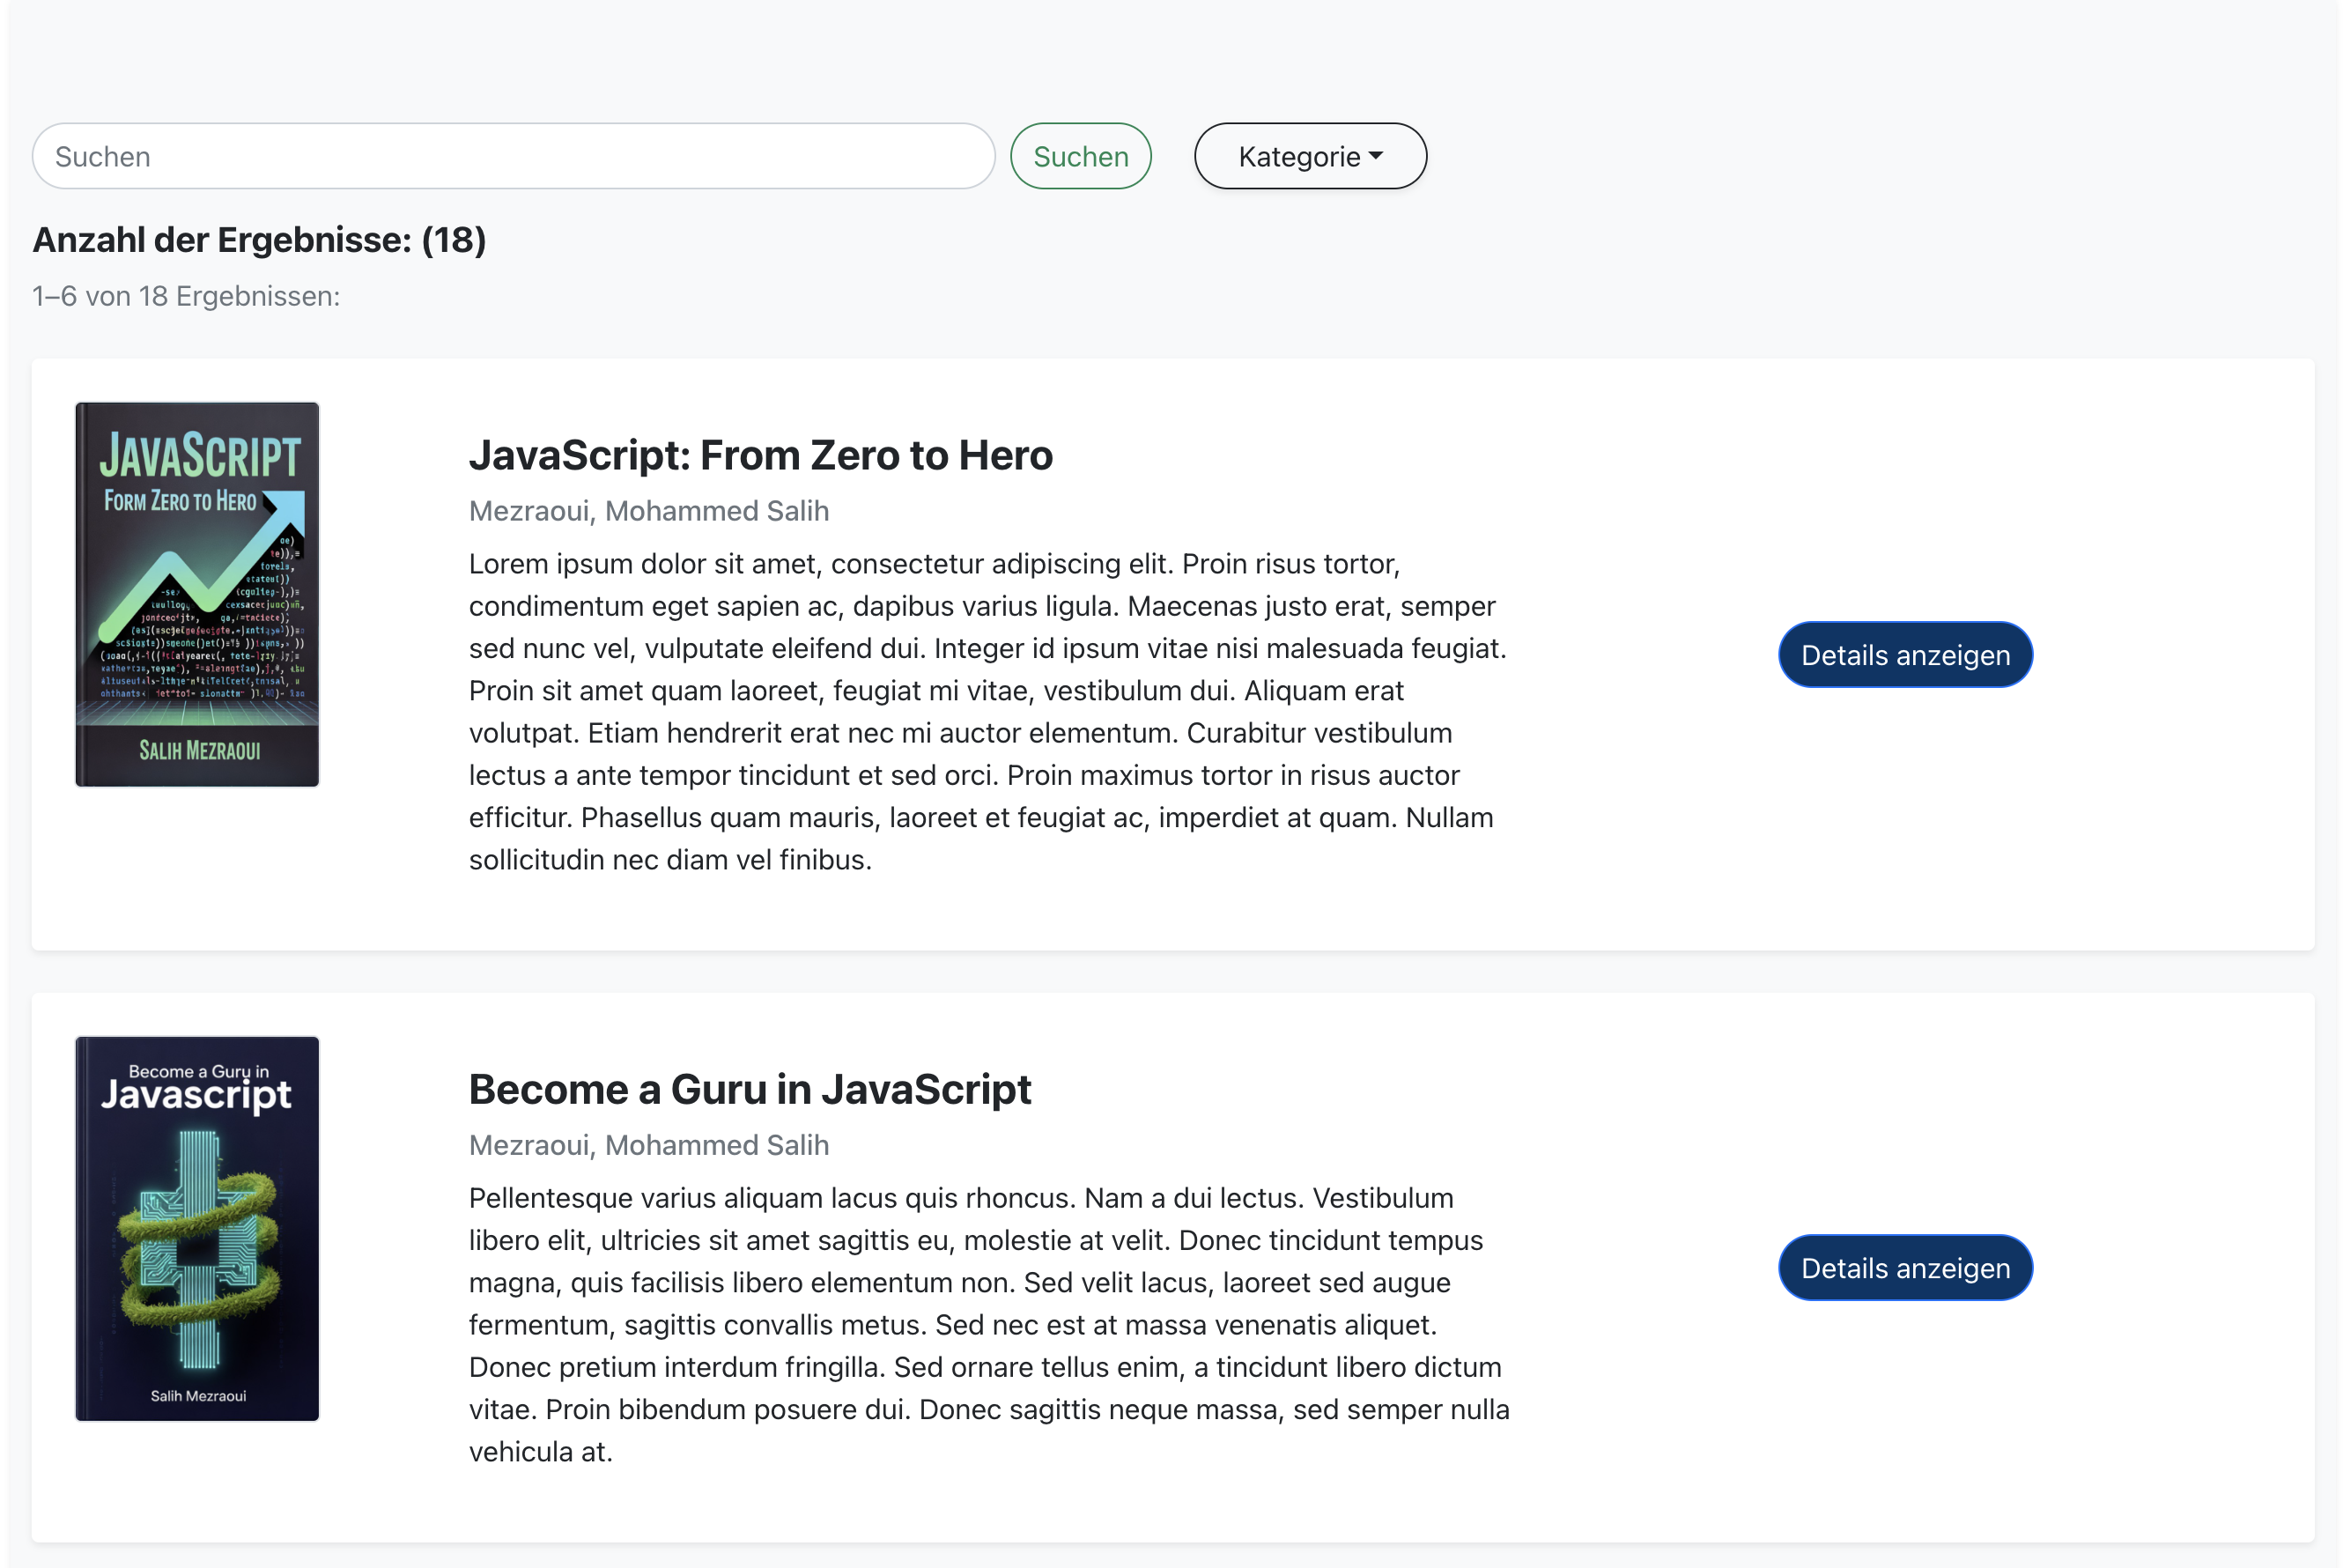
\includegraphics[width=1.0\textwidth]{images/UI-screenshots/Search-page.png}%\subsection{Startseite (Main Page)}
	\caption{Benutzeroberfläche der Suchseite}
	\label{fig:Search-page}
\end{figure}

\subsection{Buchseite}
Die untenstehende Abbildung  \ref{fig:Book-page} zeigt die Benutzeroberfläche der Buchseite. 

\begin{figure}[H]
	\centering
	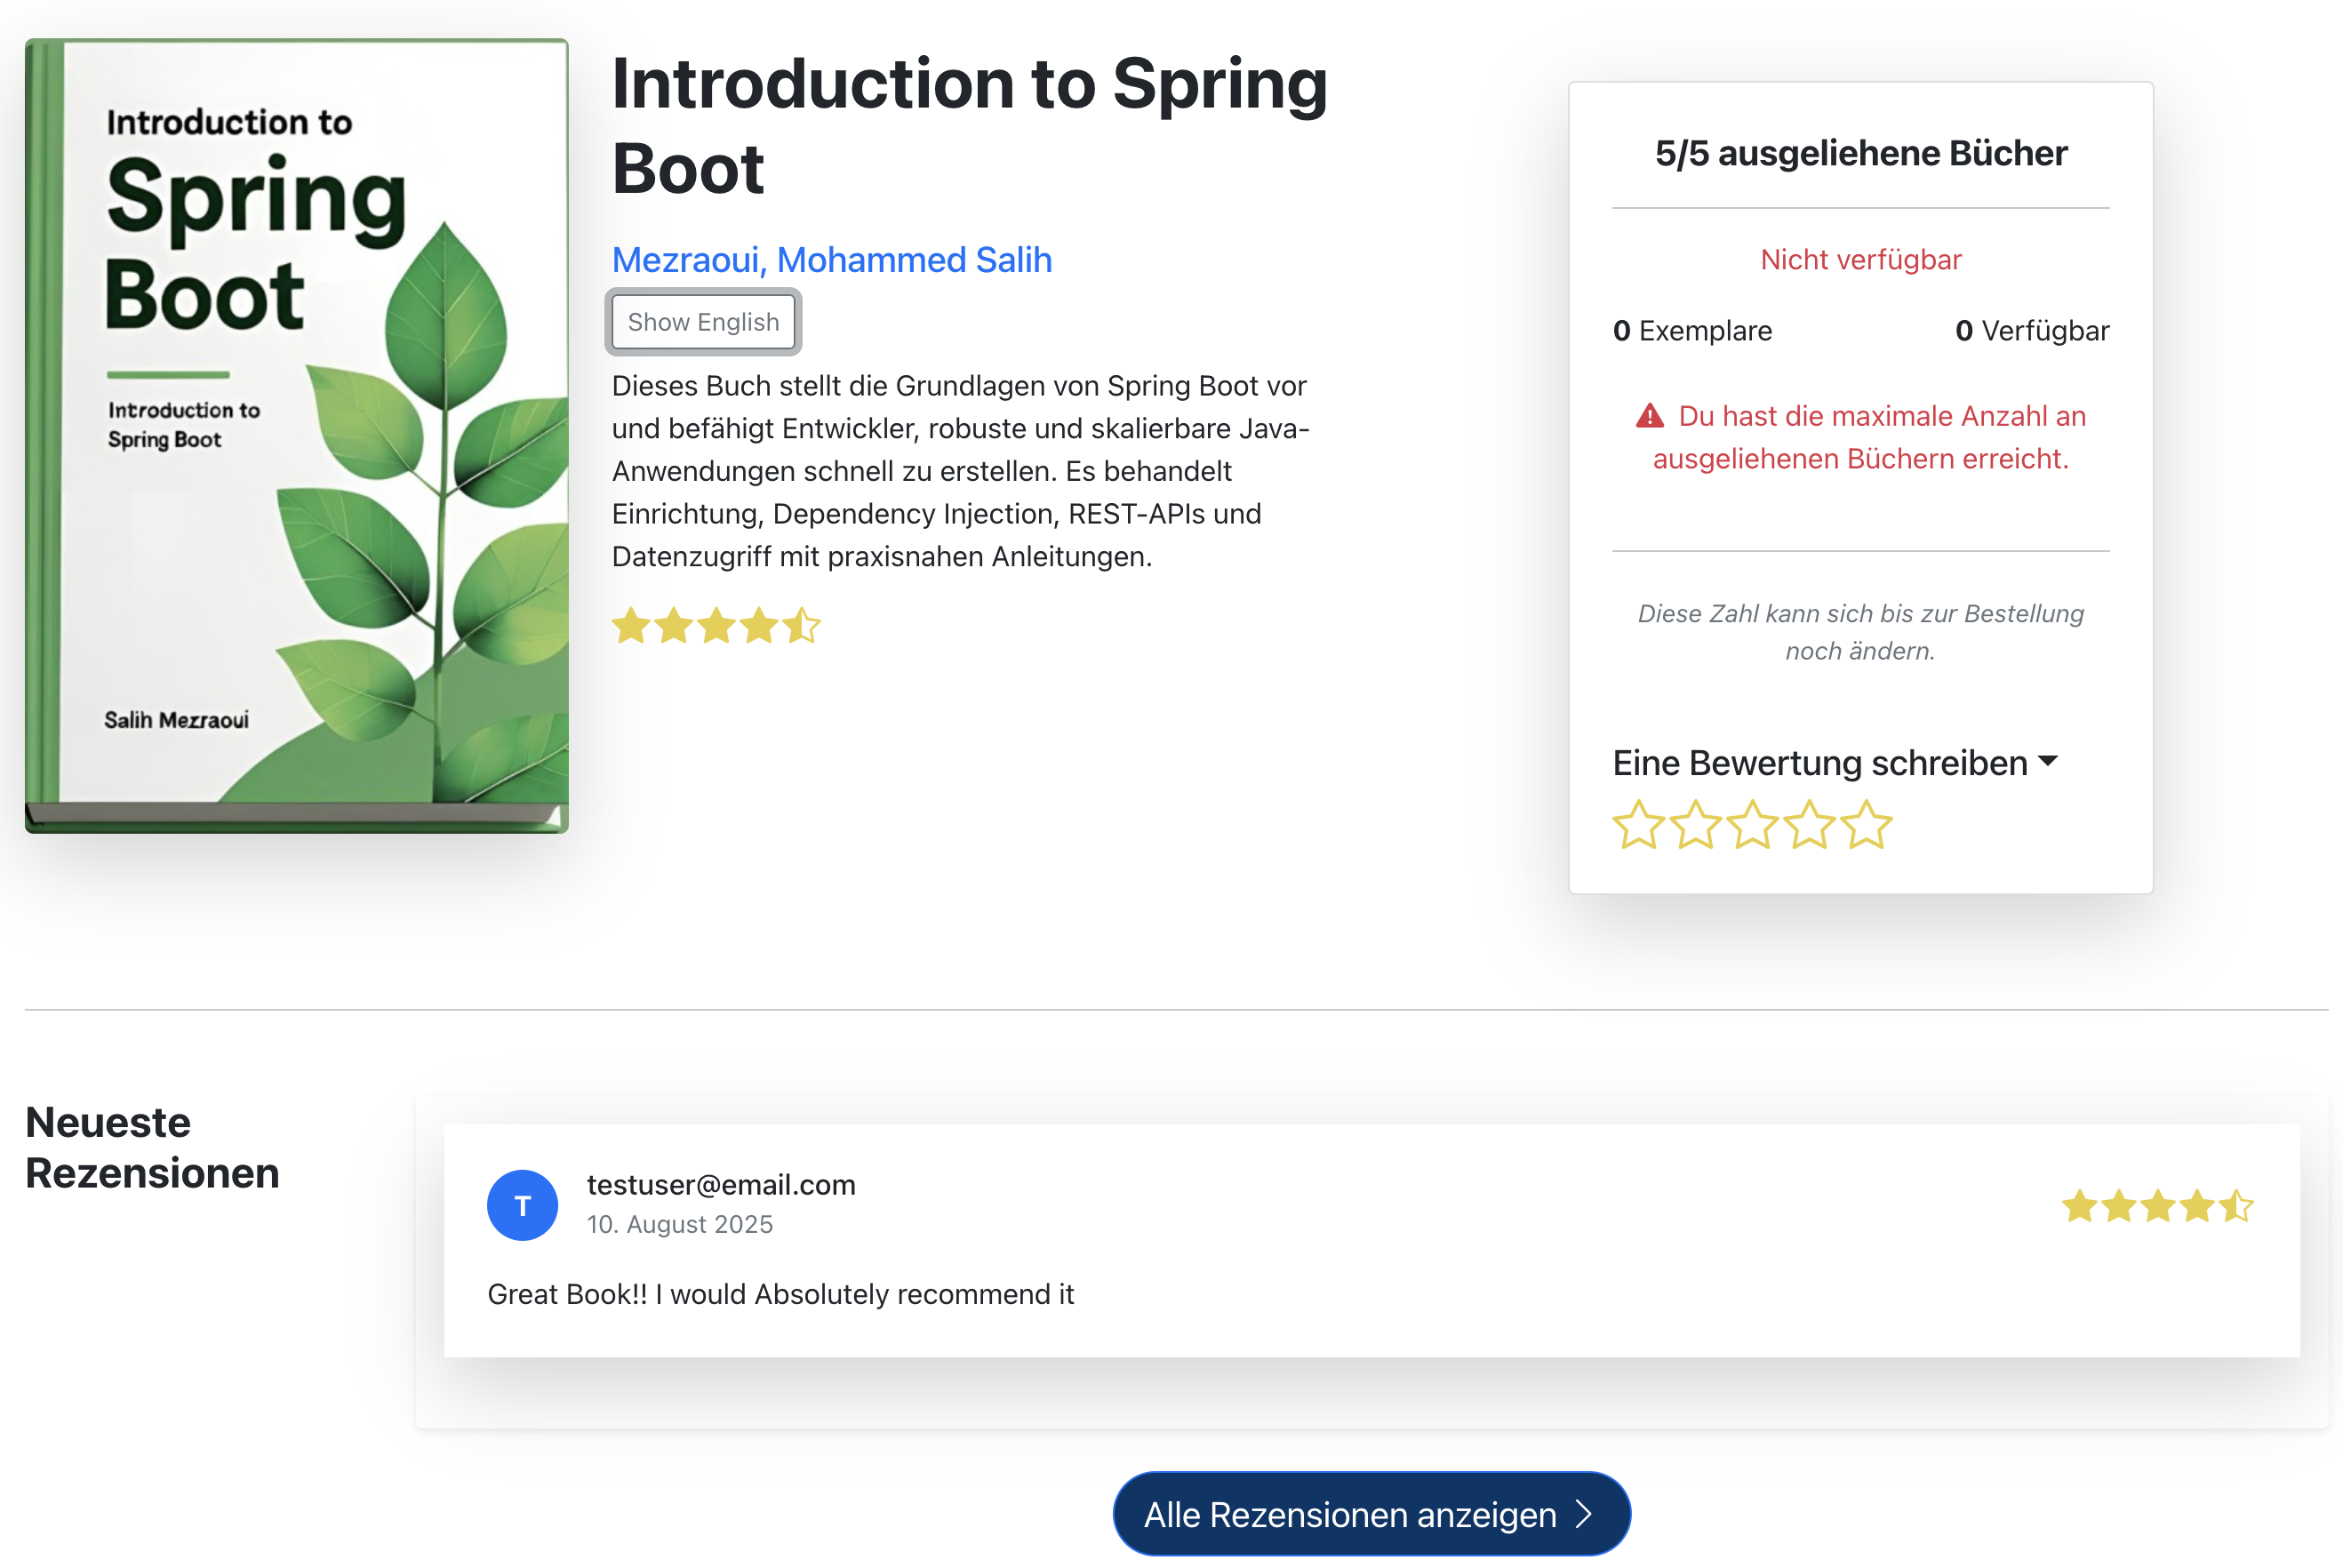
\includegraphics[width=1.0\textwidth]{images/UI-screenshots/Book-Page.png}
	\caption{Benutzeroberfläche der Buchseite}
	\label{fig:Book-page}
\end{figure}

\noindent Die Buchdetailseite stellt umfassende Informationen zu einem einzelnen Buch bereit und enthält folgende Elemente:
\begin{itemize}
	\item Darstellung des Buchcovers.
	\item Anzeige des Buchtitels und des Autors.
	\item Buchbeschreibung mit der Möglichkeit, zwischen deutscher und englischer Sprache zu wechseln, unabhängig von der Spracheinstellung der Gesamtanwendung.
	\item Bewertungssystem zur Anzeige der durchschnittlichen Nutzerbewertung.
	\item Rechte Seitenleiste mit folgenden Informationen:
	\begin{itemize}
		\item Anzahl der vom aktuellen Benutzer ausgeliehenen Exemplare,
		\item Anzahl der derzeit verfügbaren Exemplare,
		\item Gesamtanzahl der im Bestand befindlichen Exemplare.
	\end{itemize}
	\item Übersicht der Nutzerbewertungen zum Buch.
	\item Link zur vollständigen Liste aller Reviews.
\end{itemize}

\section{Bibliotheksaktivität}
In diesem Abschnitt werden die Funktionen zur Verwaltung aktueller und vergangener Ausleihen dargestellt.

\subsection{Ausleihen}
Die untenstehende Abbildung \ref{fig:Loans-Page} zeigt das Design der \texttt{Ausleihen} Seite. 

\begin{figure}[H]
	\centering
	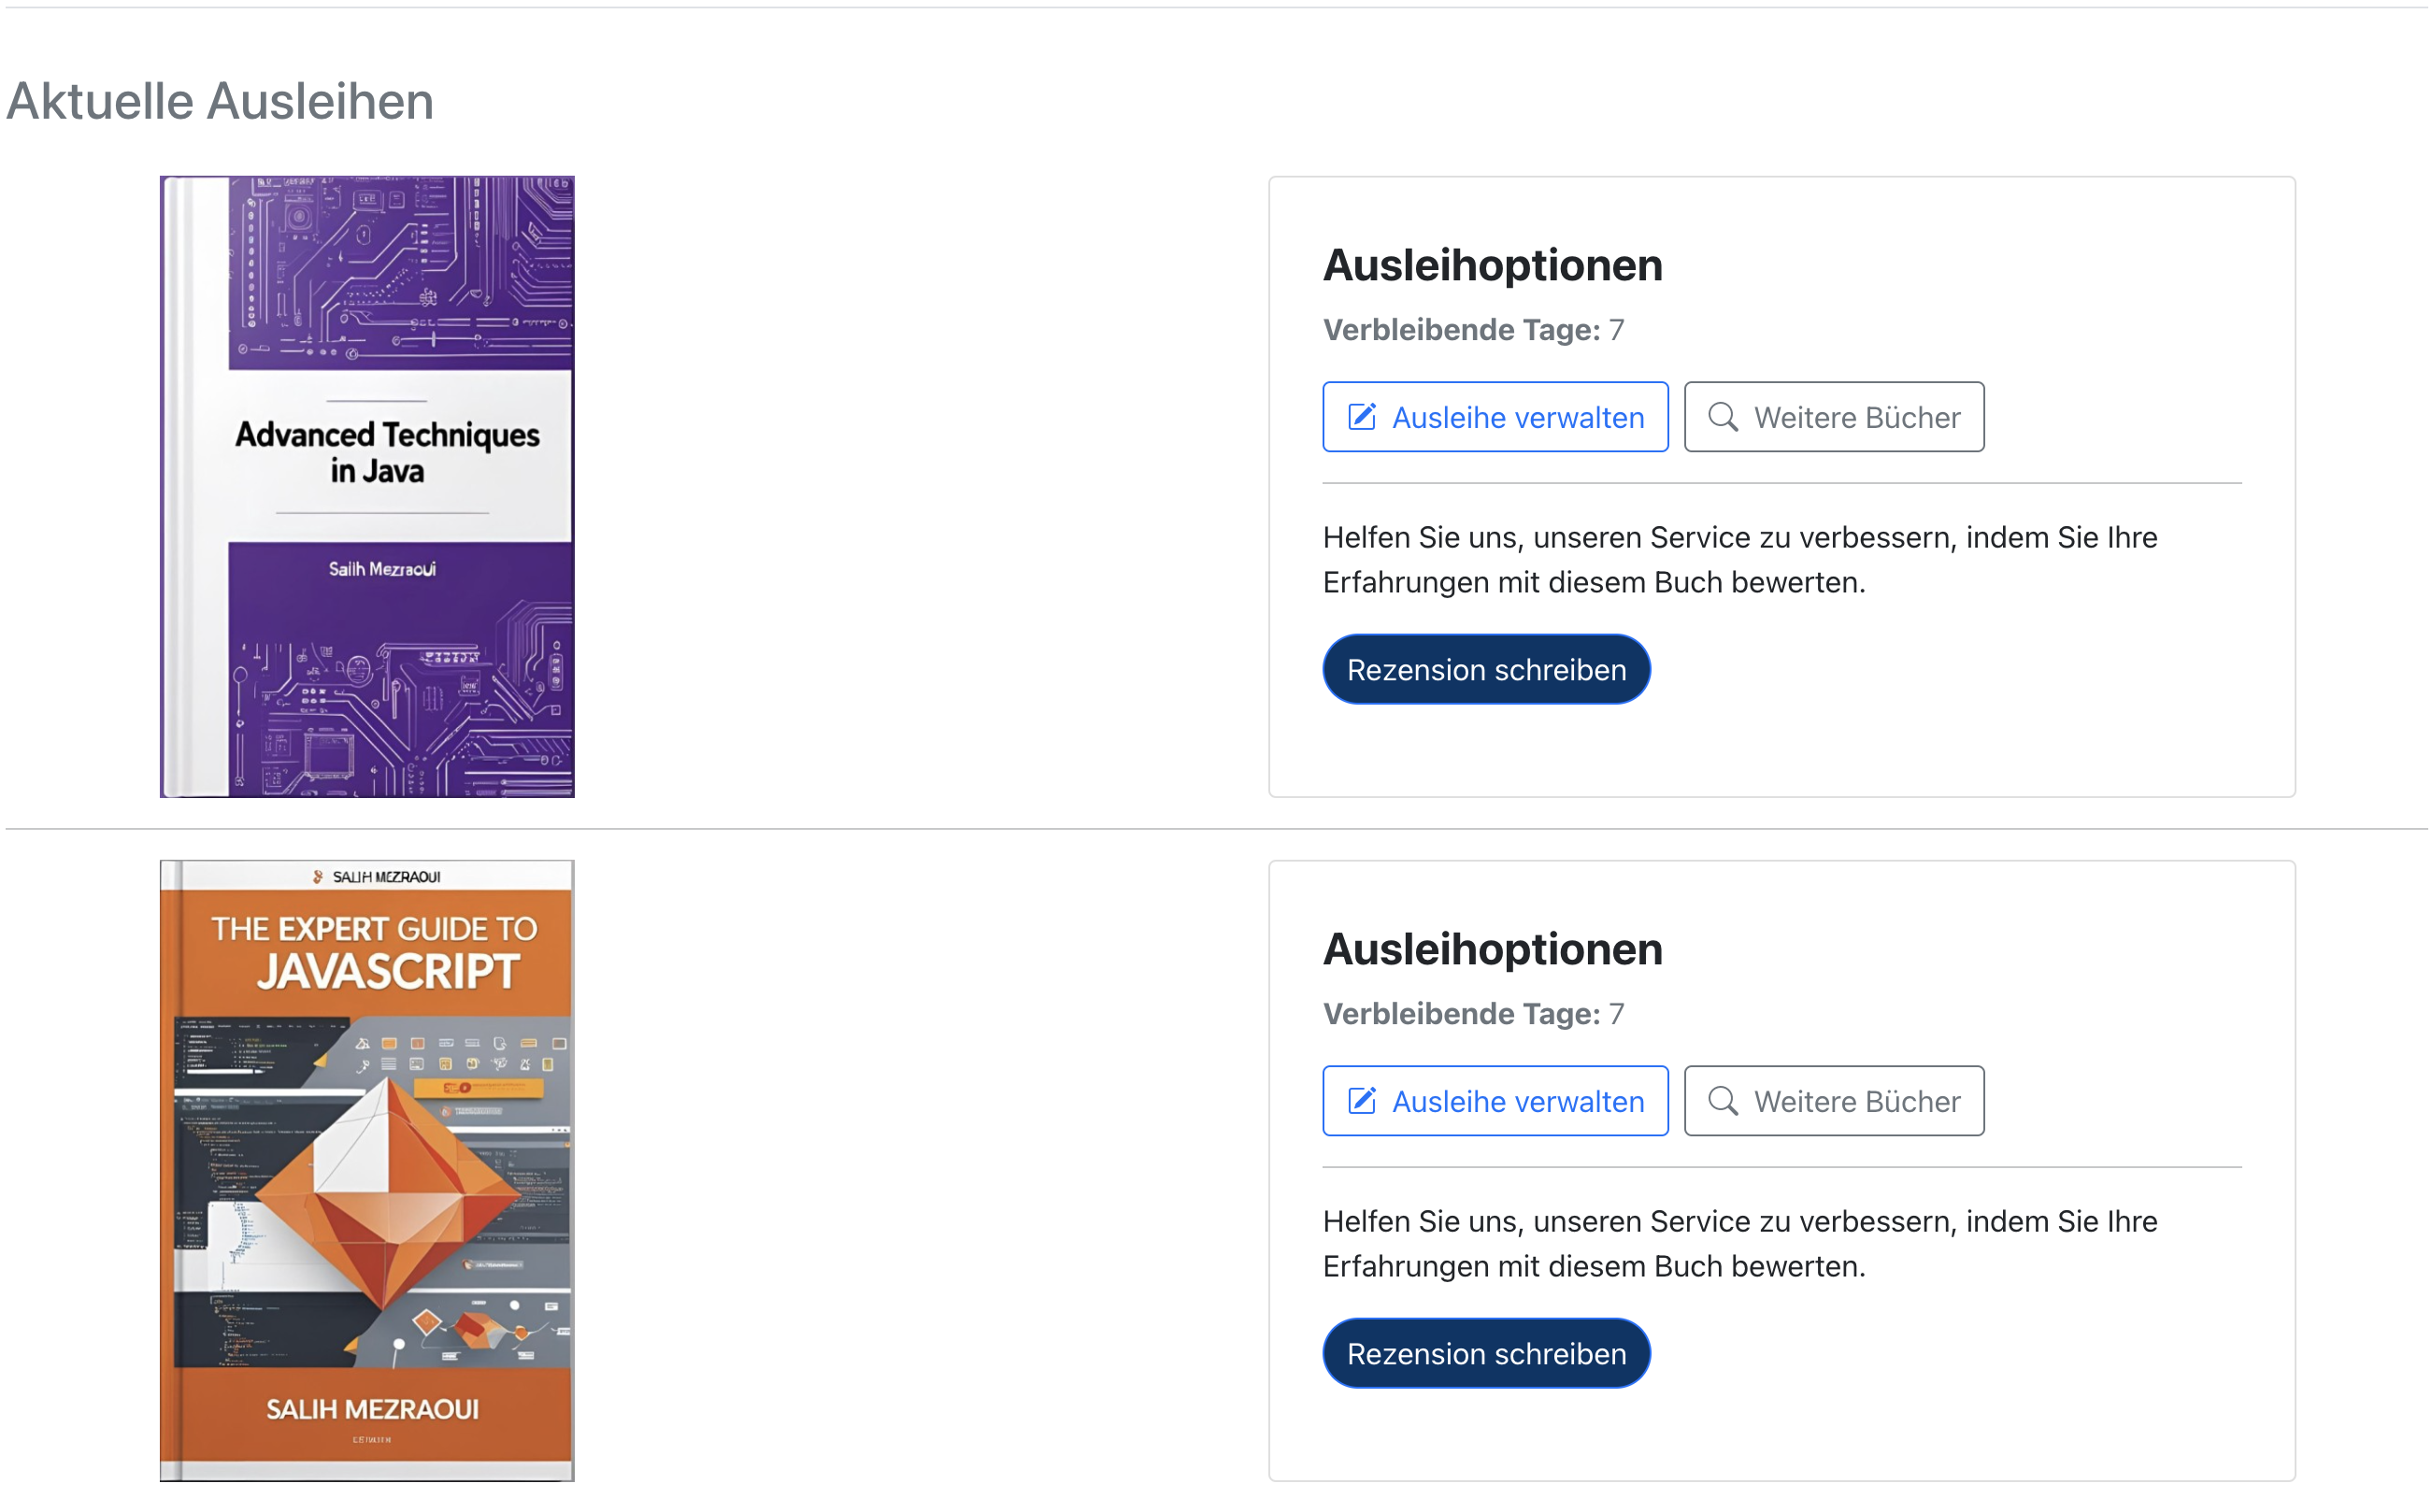
\includegraphics[width=1.0\textwidth]{images/UI-screenshots/Loans-Page.png}
	\caption{Benutzeroberfläche der Ausleihseite}
	\label{fig:Loans-Page}
\end{figure}

Die Ausleiheseite ermöglicht es Nutzerinnen und Nutzern, ihre aktuell ausgeliehenen Bücher zu verwalten. Sie enthält folgende Elemente:

\begin{itemize}
	\item Liste aller aktuell ausgeliehenen Bücher.
	\item Anzeige der verbleibenden Tage bis zur Rückgabe jedes Buches.
	\item Verwaltungsoptionen pro Buch:
	\begin{itemize}
		\item Rückgabe des Buches,
		\item Verlängerung der Leihfrist.
	\end{itemize}
	\item Schaltfläche zur Suche nach weiteren Büchern.
	\item Link zum Verfassen einer Rezension für das jeweilige Buch.
\end{itemize}

\subsection{Ausleihhistorie}
Die untenstehende Abbildung \ref{fig:Loans-History-Page} zeigt das Design der Seite \texttt{Ausleihverlauf}. Diese Seite enthält die Historie der vom Nutzer ausgeliehenen Bücher, einschließlich des Ausleih- und Rückgabedatums.

\begin{figure}[H]
	\centering
	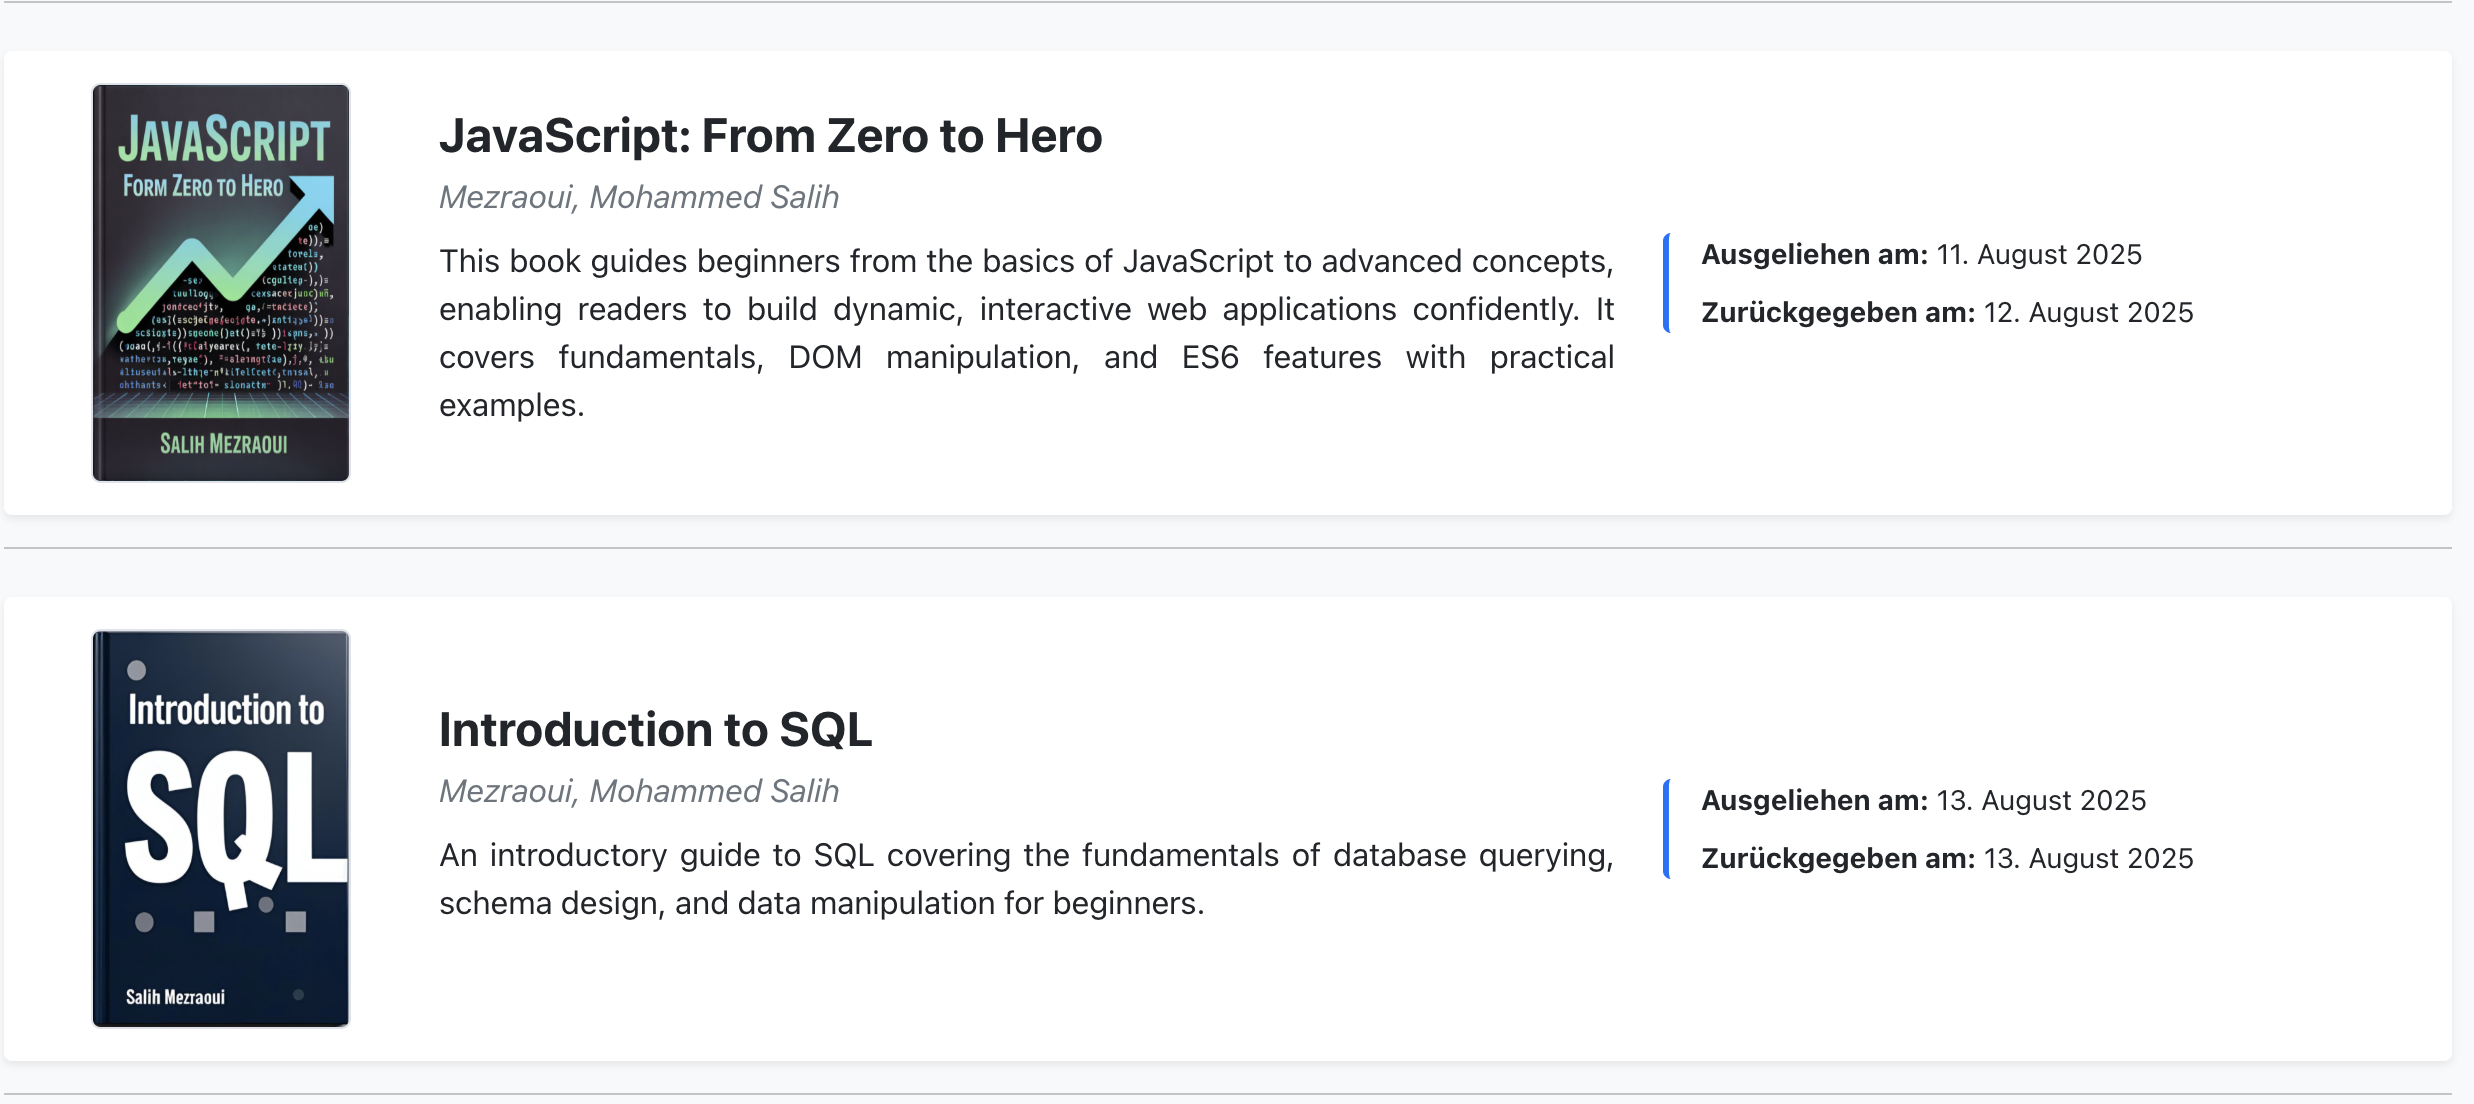
\includegraphics[width=1.0\textwidth]{images/UI-screenshots/Loans-History.png}
	\caption{Benutzeroberfläche der Ausleihverlaufsseite}%\subsection{Bibliotheksservice (Library Service)}
	\label{fig:Loans-History-Page}
\end{figure}

\section{Bibliotheksdienste}
In diesem Abschnitt werden die Bibliotheksdienste vorgestellt, insbesondere die Benutzeroberfläche zur Übermittlung von Anfragen sowie der persönliche Nachrichtenverlauf mit den jeweiligen Antworten.

\noindent Die folgende Abbildung \ref{fig:Message-Send} zeigt die Benutzeroberfläche, über die Benutzer einzelne Anfragen oder Nachrichten an die Administratoren der Bibliothek senden können.

\begin{figure}[H]
	\centering
	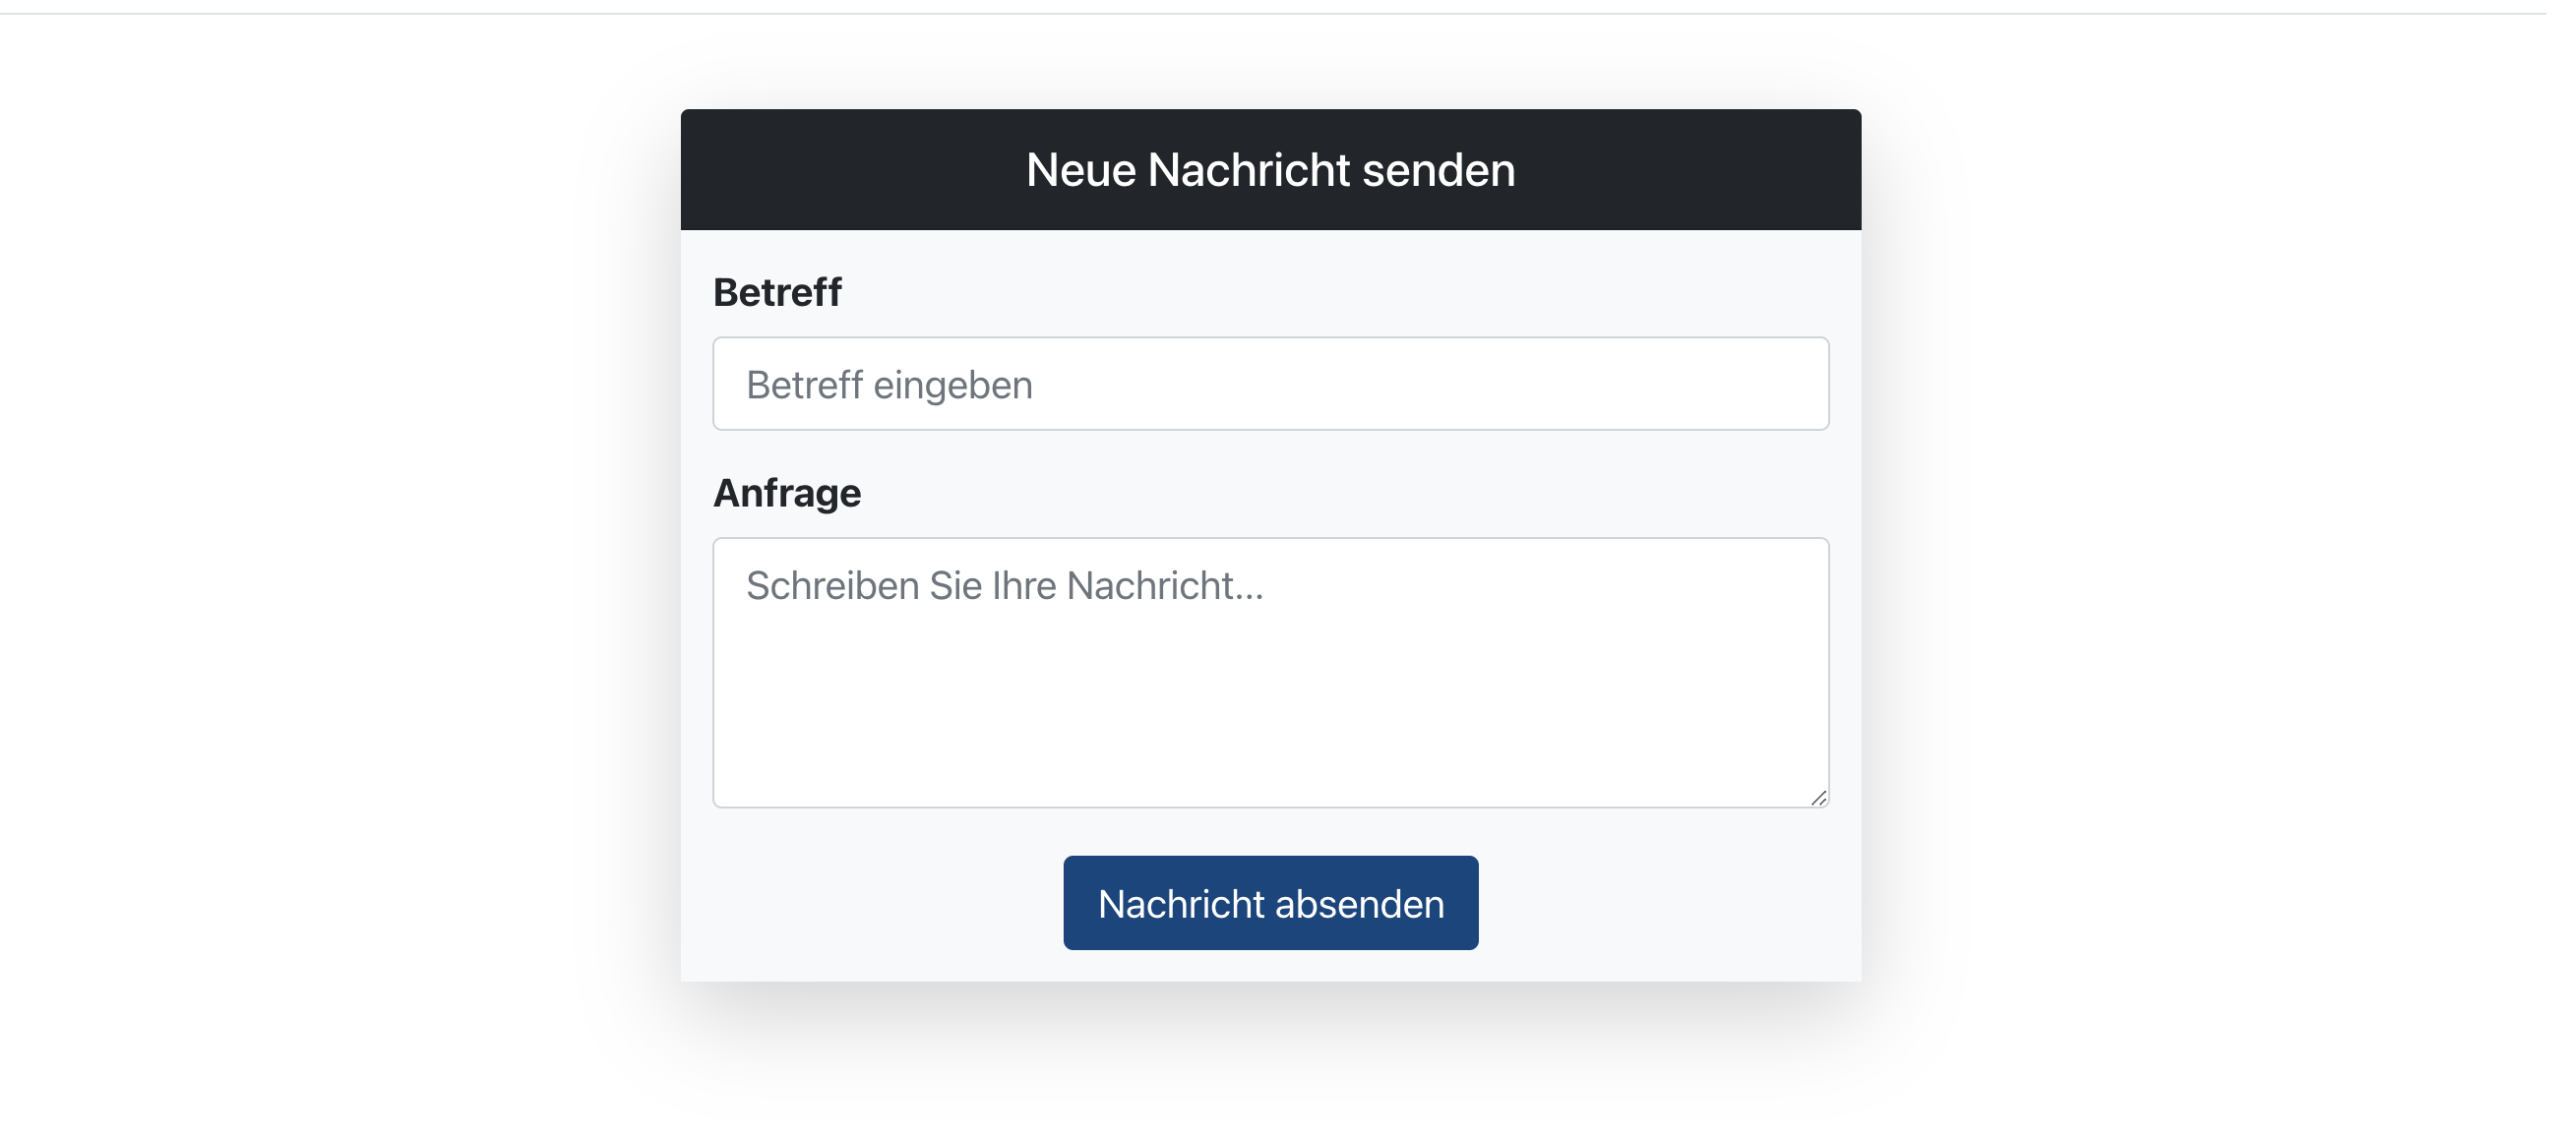
\includegraphics[width=1.0\textwidth]{images/UI-screenshots/Message-Send.png}
	\caption{Benutzeroberfläche zum Versenden von Anfragen}
	\label{fig:Message-Send}
\end{figure}

\noindent Die Abbildung \ref{fig:Messages-History} veranschaulicht den Verlauf sämtlicher ausgetauschter Nachrichten, einschließlich der gestellten Fragen und der dazugehörigen Antworten.

\begin{figure}[H]
	\centering
	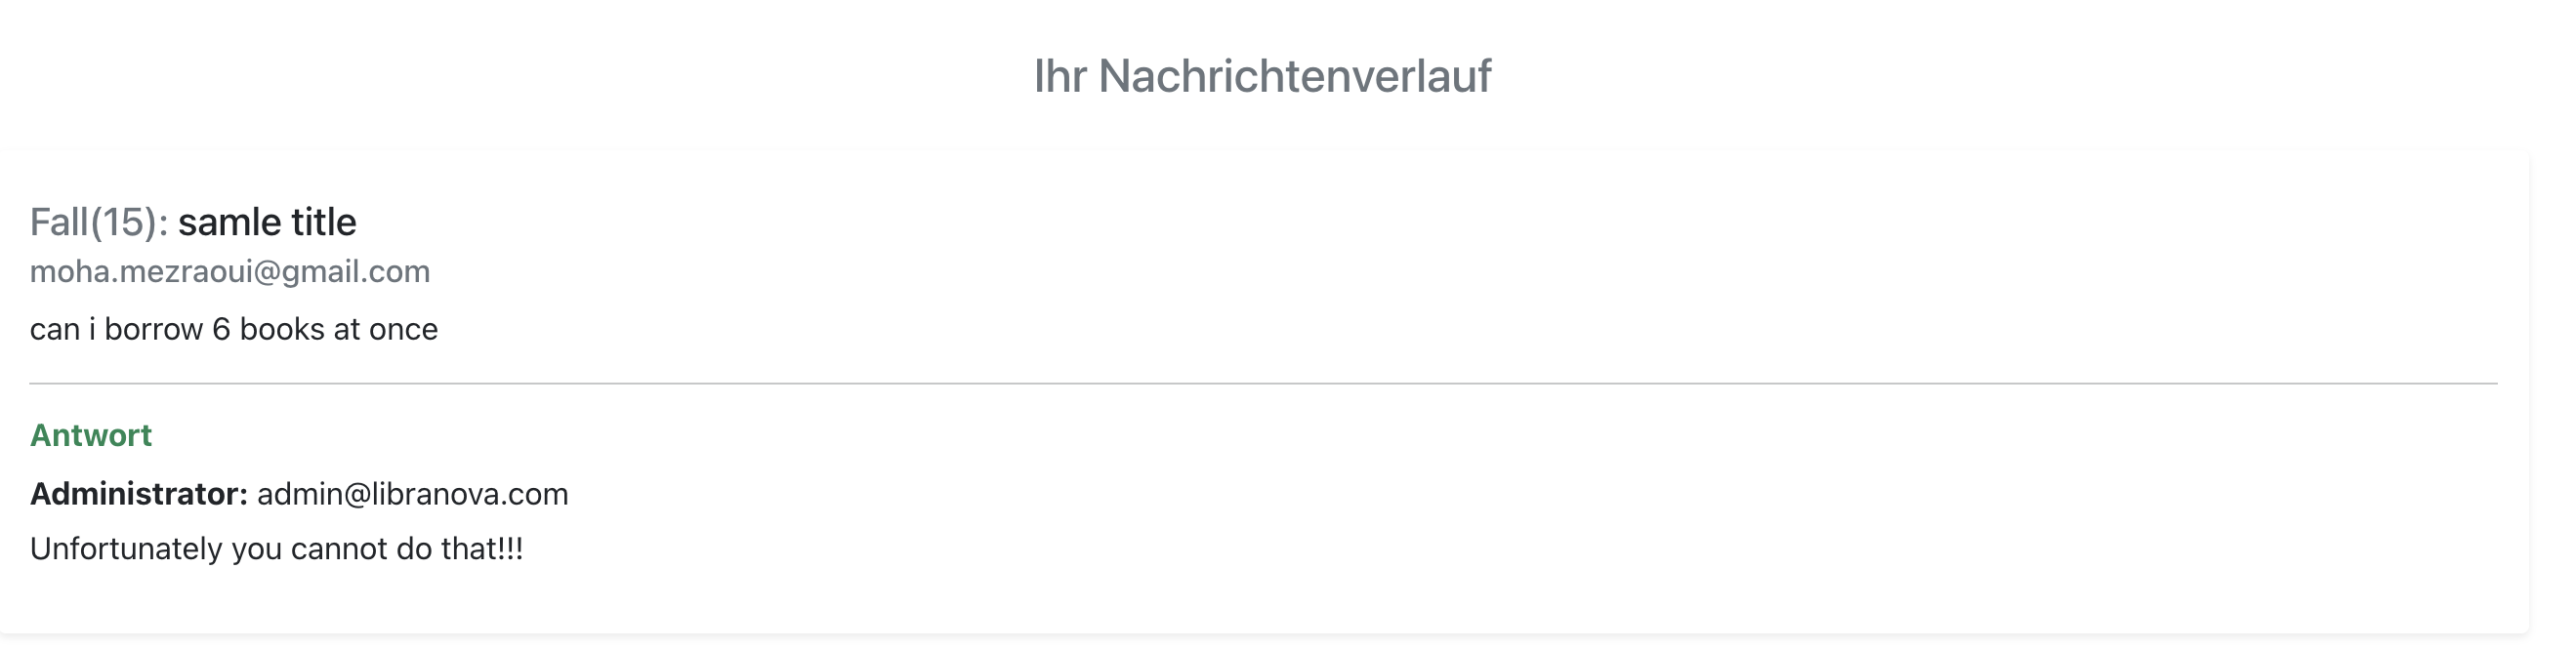
\includegraphics[width=1.0\textwidth]{images/UI-screenshots/Messages-History.png}
	\caption{Nachrichtenverlauf zwischen Nutzer und Bibliothek}
	\label{fig:Messages-History}
\end{figure}

\section{Bezahlungsseite}

In diesem Abschnitt wird die Benutzeroberfläche zur Verwaltung von Zahlungsinformationen und offenen Gebühren vorgestellt. \\

\noindent Abbildung \ref{fig:Outstanding-payment} zeigt das Layout, das angezeigt wird, wenn ein Benutzer ausstehende Zahlungen zu begleichen hat. 

\begin{figure}[H]
	\centering
	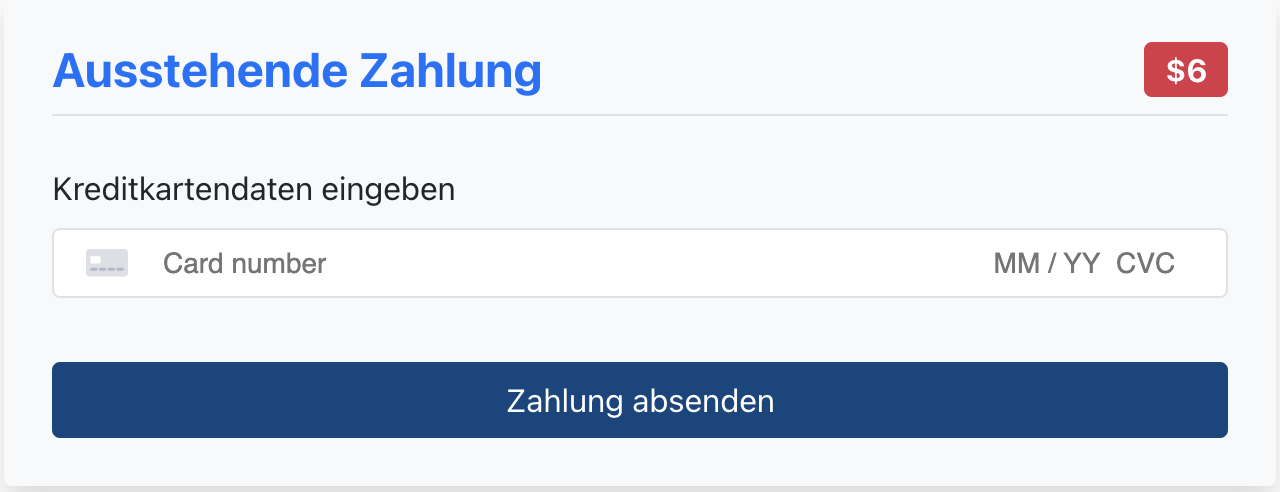
\includegraphics[width=1.0\textwidth]{images/UI-screenshots/Outstanding-payment.png}
	\caption{Benutzeroberfläche bei ausstehenden Zahlungen}
	\label{fig:Outstanding-payment}
\end{figure}

\noindent Wenn keine offenen Gebühren vorliegen, wird dem Nutzer die in Abbildung \ref{fig:No-Payment} dargestellte Ansicht präsentiert. Sie bestätigt, dass derzeit keine Zahlungen erforderlich sind.

\begin{figure}[H]
	\centering
	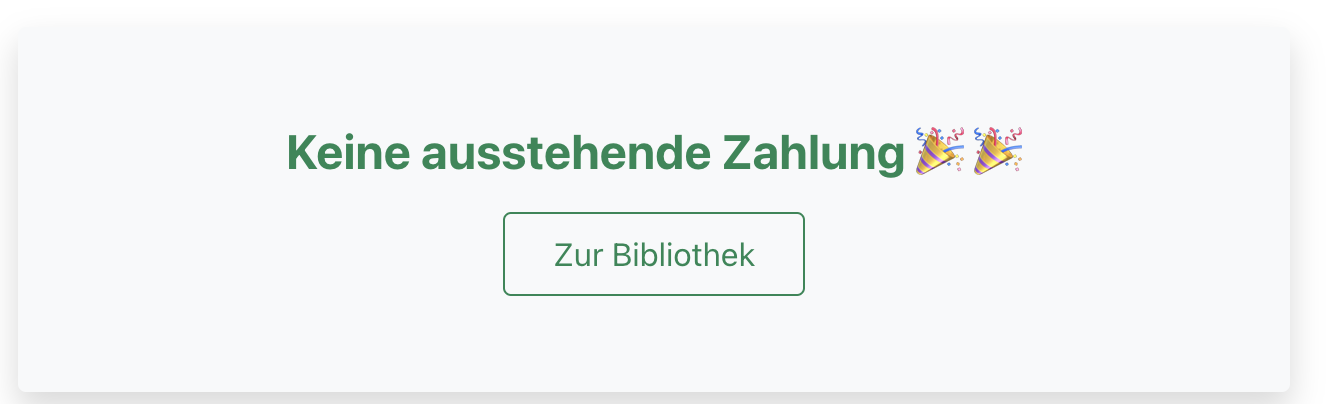
\includegraphics[width=1.0\textwidth]{images/UI-screenshots/No-Payment.png}
	\caption{Benutzeroberfläche bei keinen offenen Zahlungen}
	\label{fig:No-Payment}
\end{figure}

\section{Admin-Bereich}

Der Admin-Bereich bietet eine dedizierte Oberfläche zur Verwaltung der Bibliotheksressourcen und zur Interaktion mit Benutzeranfragen. In diesem Abschnitt werden die Verwaltungsfunktionen dargestellt, die einem Administrator zur Verfügung stehen.

\subsection{Neues Buch hinzufügen}
\noindent Die erste Funktion (siehe \ref{fig:Add-New-Book})ermöglicht es dem Administrator, neue Bücher in das System aufzunehmen. Hierzu gibt er relevante Informationen wie Titel, Autor, Kategorie, eine kurze Beschreibung sowie die Anzahl der verfügbaren Exemplare an. Zusätzlich kann ein Bild des Buchcovers hochgeladen werden. Nach dem Ausfüllen der Felder wird durch Klicken auf die Schaltfläche \textit{"Buch hinzufügen"} ein neuer Eintrag erstellt.
\begin{figure}[H]
	\centering
	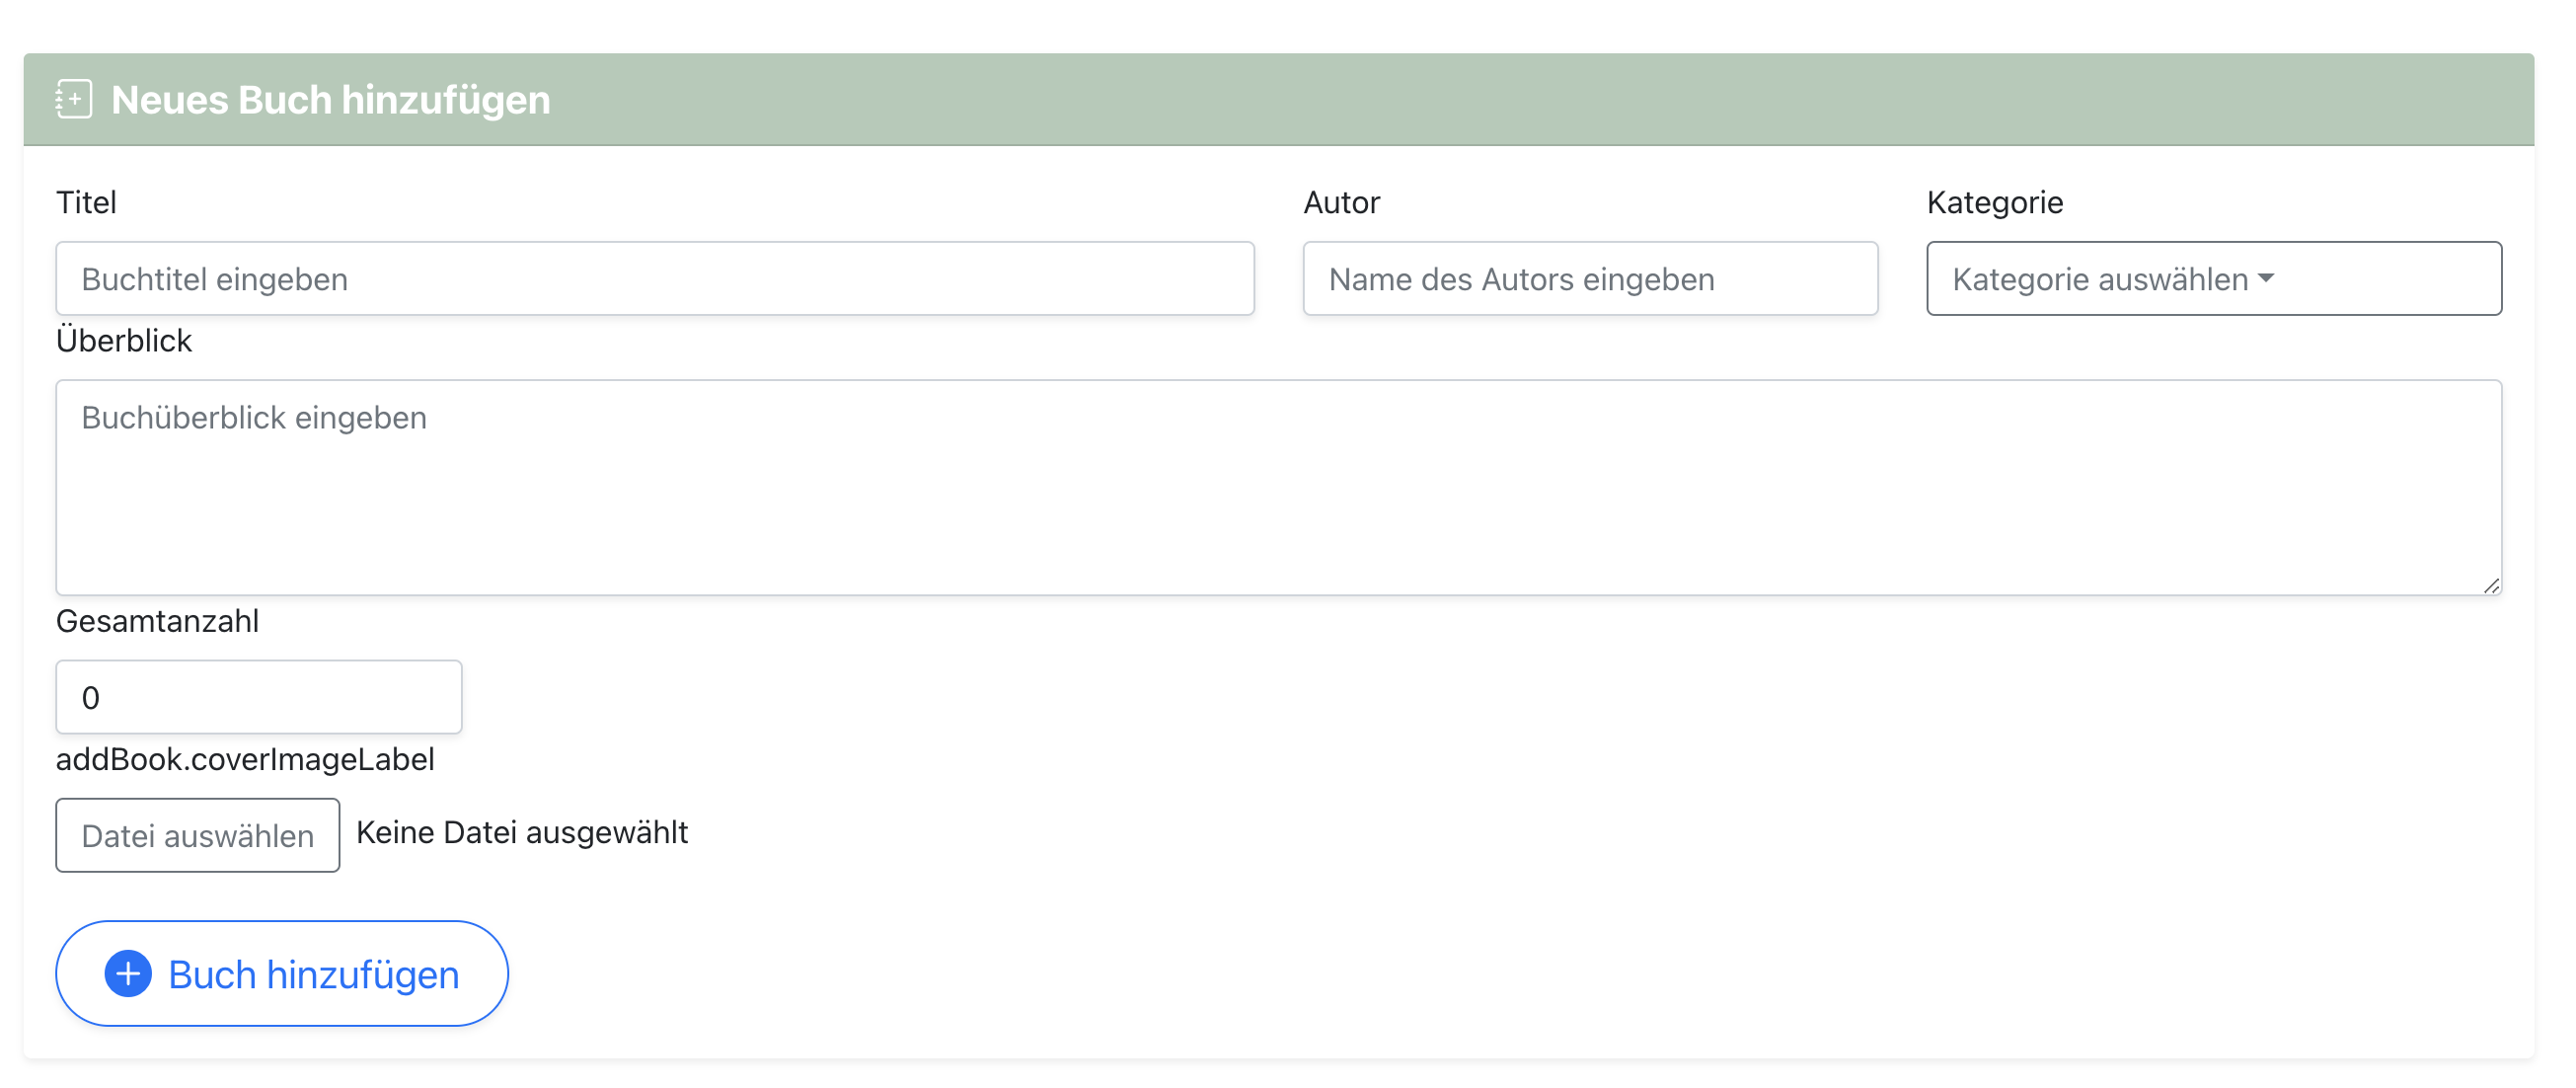
\includegraphics[width=1.0\textwidth]{images/UI-screenshots/Add-New-Book.png}
	\caption{Benutzeroberfläche bei keinen offenen Zahlungen}
	\label{fig:Add-New-Book}
\end{figure}

\subsection{Bücher verwalten}

\noindent Der Administrator kann bestehende Bücher verwalten, indem er die Anzahl der verfügbaren Exemplare anpasst oder Bücher vollständig aus dem System entfernt. Die folgende Abbildung \ref{fig:Manage-Books} zeigt die Verwaltungsoberfläche, über die solche Änderungen vorgenommen werden können.

\begin{figure}[H]
	\centering
	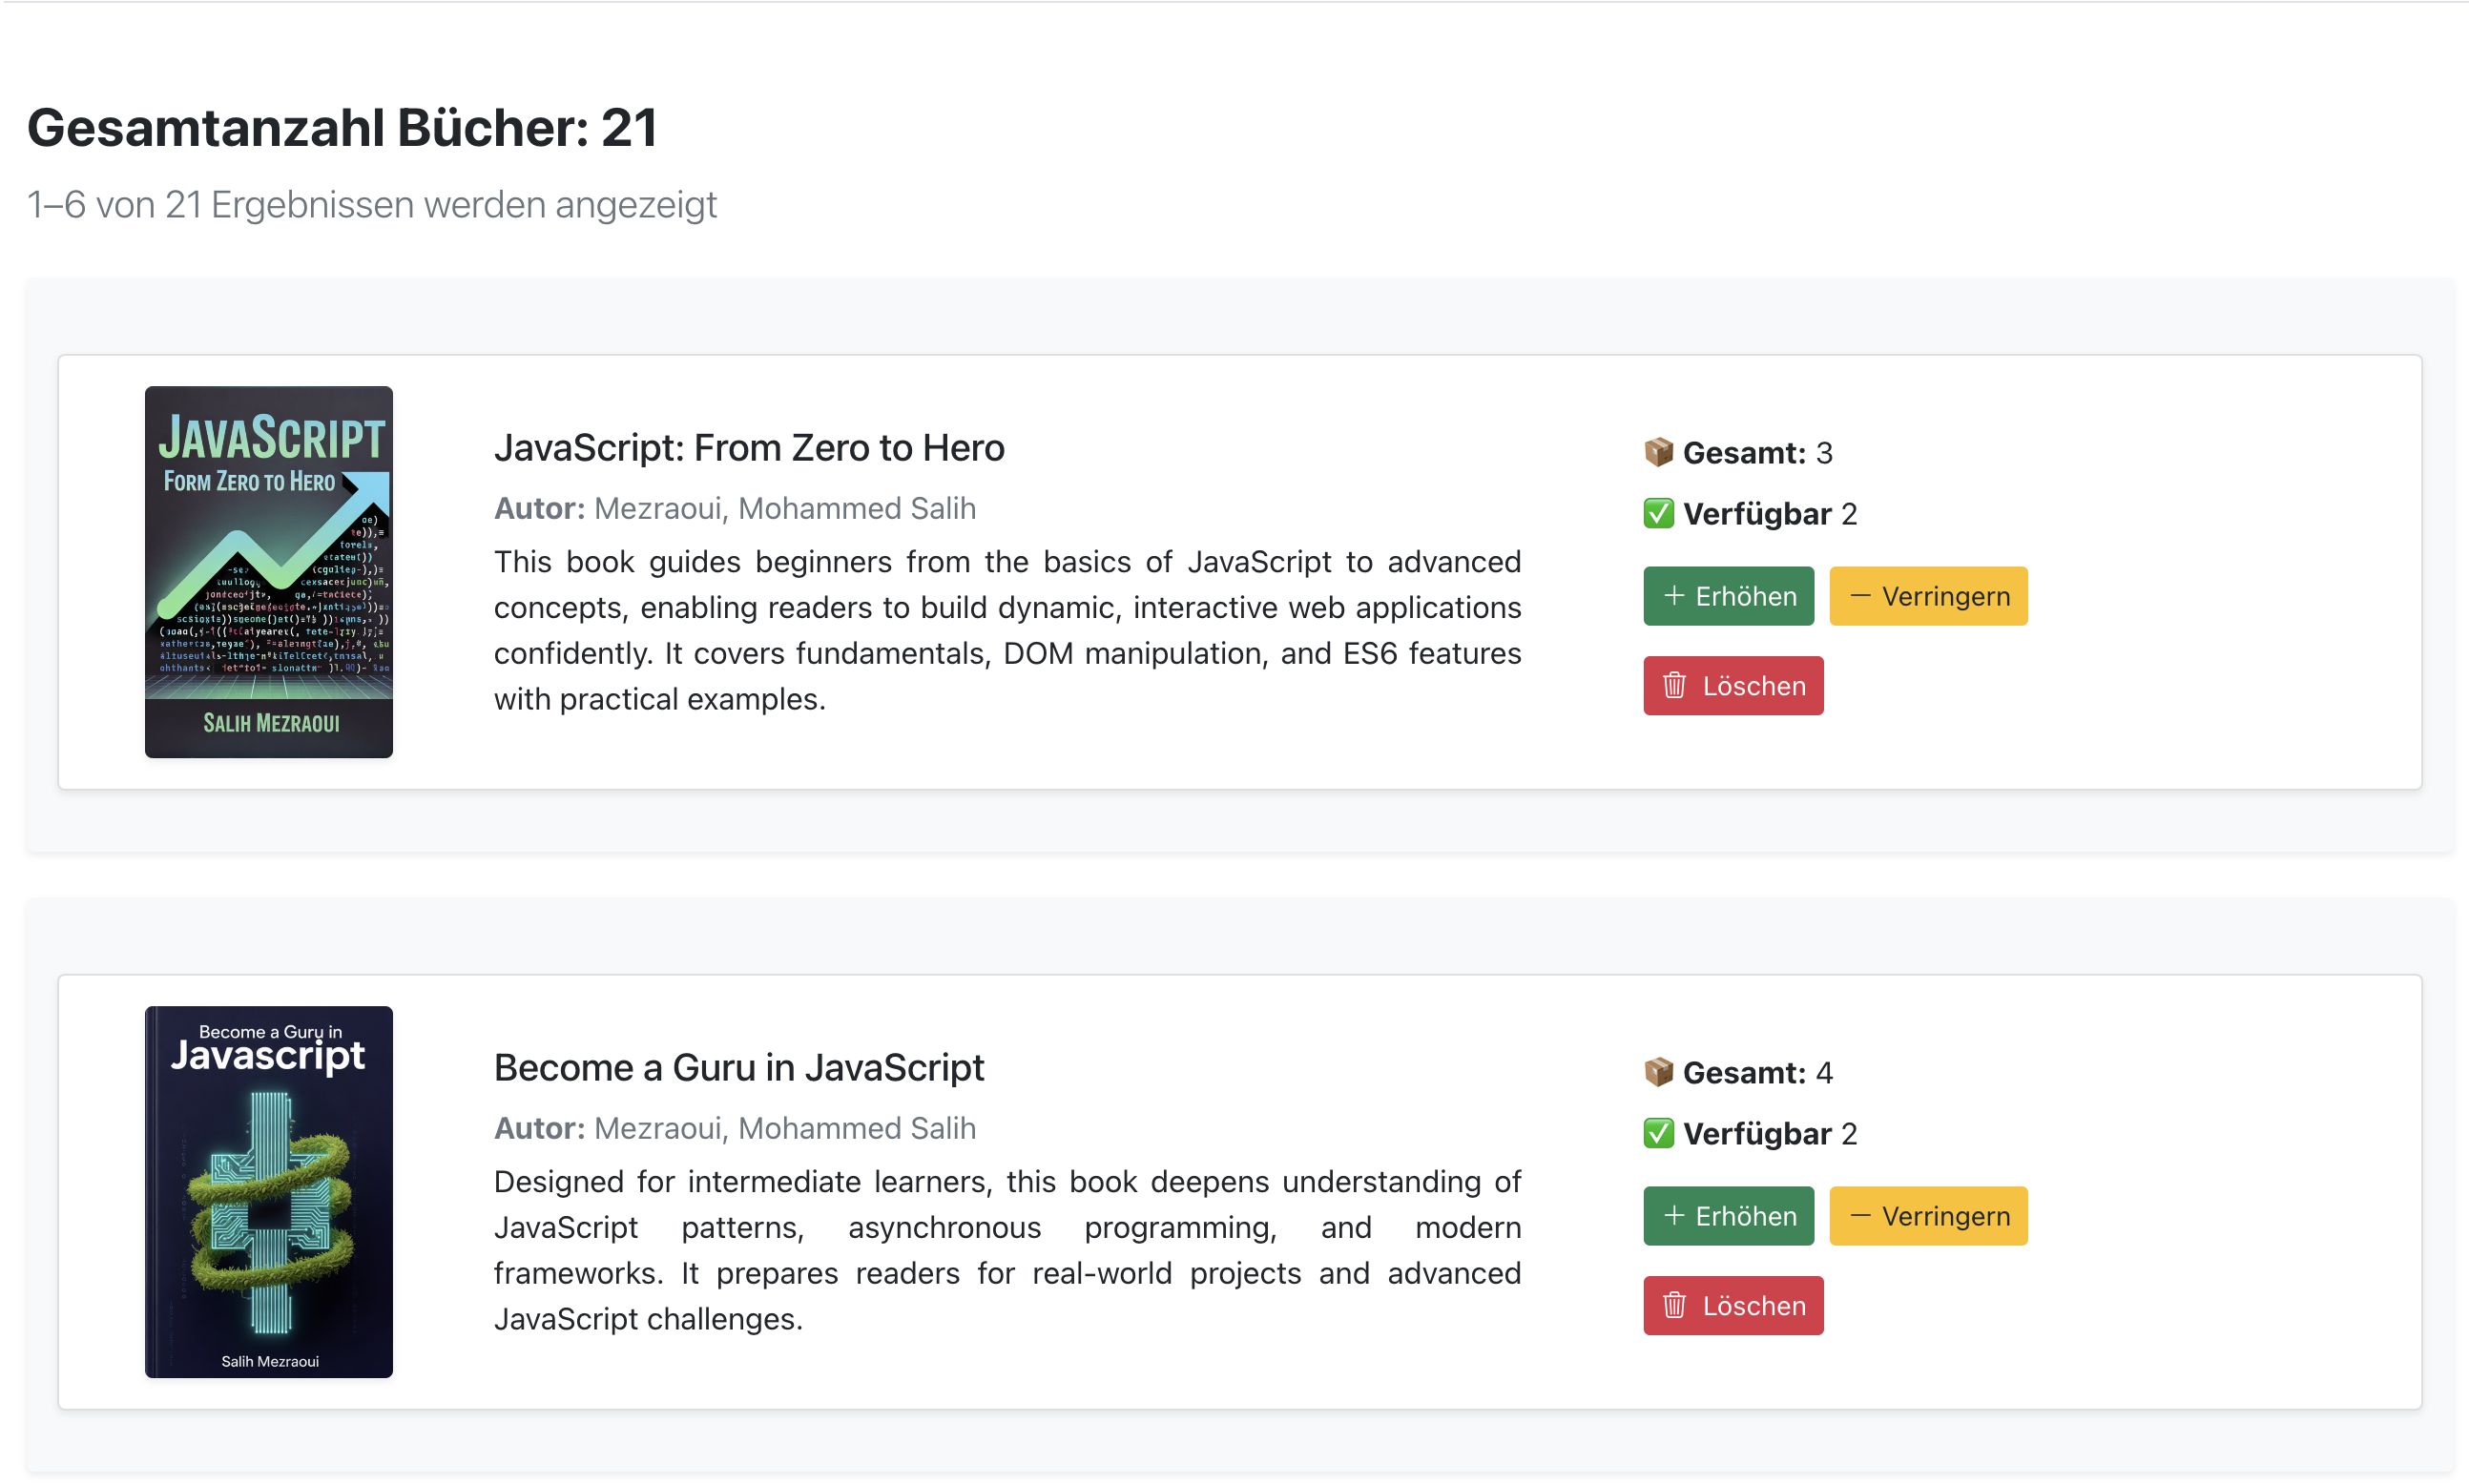
\includegraphics[width=1.0\textwidth]{images/UI-screenshots/Manage-Books.png}
	\caption{Benutzeroberfläche bei keinen offenen Zahlungen}
	\label{fig:Manage-Books}
\end{figure}
\subsection{Nachrichten}

\noindent In diesem Bereich kann der Administrator auf Anfragen von Benutzern antworten. Die Benutzerfrage wird angezeigt und kann direkt über das vorgesehene Textfeld beantwortet werden. Eine Schaltfläche ermöglicht das Senden der Antwort. Die Abbildung \ref{fig:Messages-Responses} zeigt die zugehörige Benutzeroberfläche.

\begin{figure}[H]
	\centering
	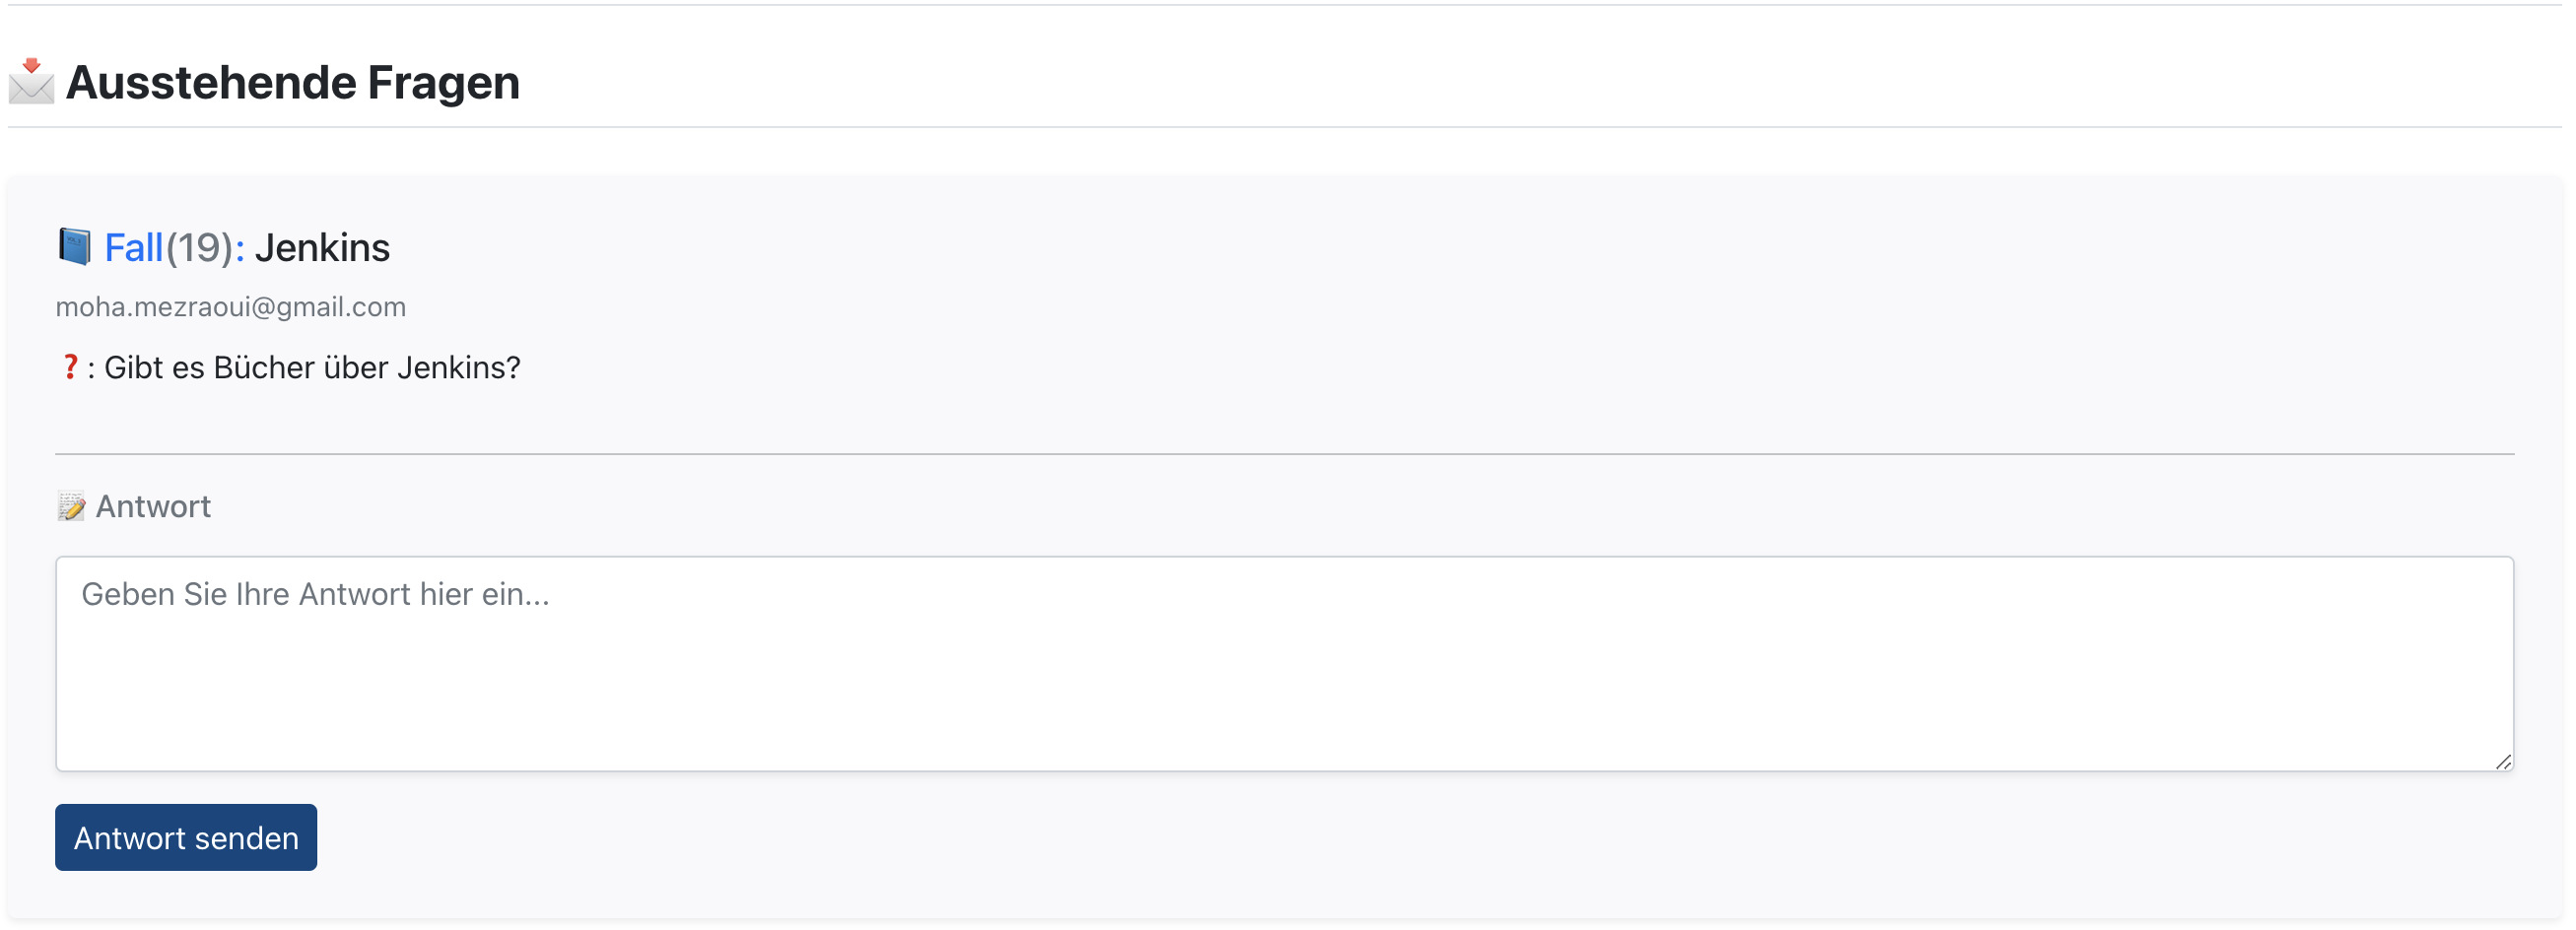
\includegraphics[width=1.0\textwidth]{images/UI-screenshots/Messages-Responses.png}
	\caption{Benutzeroberfläche bei keinen offenen Zahlungen}
	\label{fig:Messages-Responses}
\end{figure}





















\chapter{Anwendungsszenarien}

Die im Rahmen dieses Projekts entwickelte Anwendung zur Verwaltung von Büchern ist flexibel einsetzbar und bietet zahlreiche Erweiterungsmöglichkeiten über den ursprünglichen Anwendungsfall hinaus. Dank ihrer modularen Architektur, der Nutzung von REST-APIs und der durchdachten Benutzeroberfläche lässt sich das System leicht an verschiedene Nutzungsszenarien anpassen.

\noindent Im Folgenden werden exemplarisch mehrere Anwendungsbereiche vorgestellt, in denen das System sinnvoll eingesetzt oder erweitert werden könnte. Dazu zählen insbesondere der Bildungsbereich und E-Learning-Plattformen, die mobile Nutzung durch Erweiterung zu nativen Apps sowie innovative Funktionen wie personalisierte Buchempfehlungen, Fernleihe sowie Echtzeit-Reservierungsbenachrichtigungen. Diese Szenarien verdeutlichen das Potenzial des Systems, weit über die klassische Bibliotheksverwaltung hinaus einen Mehrwert für Nutzerinnen und Nutzer zu schaffen.

\section{Bildungs- und E-Learning-Plattformen}\index{Bildungs- und E-Learning-Plattformen}

E-Learning-Plattformen und Bildungseinrichtungen könnten das entwickelte System als Backend-Lösung zur Bereitstellung von digitalen Lernmaterialien wie Kursunterlagen, wissenschaftlichen Artikeln oder Videoinhalten nutzen. Die integrierte Bewertungs- und Kommentarfunktion ermöglicht es Lernenden, Inhalte zu bewerten und Rezensionen zu verfassen, was wiederum anderen Nutzerinnen und Nutzern bei der Auswahl geeigneter Materialien hilft. Das System könnte zudem erweitert werden, um PDF-Dateien, E-Books und Videos mit Download- oder Streamingrechten zu verwalten und bereitzustellen. Darüber hinaus könnten individuelle Lernpfade unterstützt werden, indem relevante Ressourcen personalisiert vorgeschlagen werden.

\section{Mobile Nutzung}\index{Mobile Nutzung}

Durch die RESTful-Architektur der Anwendung ist eine einfache Erweiterung um eine mobile App möglich. Dies ermöglicht Nutzerinnen und Nutzern, bequem von unterwegs auf ihre ausgeliehenen Bücher, Rezensionen und weiteren Inhalte zuzugreifen. Die mobile Nutzung steigert die Flexibilität und Benutzerfreundlichkeit der Anwendung erheblich, indem sie den Zugriff jederzeit und überall ermöglicht – sei es auf iOS- oder Android-Geräten.


\section{Personalisierte Empfehlungen}\index{Personalisierte Empfehlungen}

Eine zukünftige Erweiterung des Systems könnte die Implementierung KI-basierter Vorschläge sein, die Nutzerinnen und Nutzern auf Basis ihrer Lesehistorie und Präferenzen individuell zugeschnittene Buchempfehlungen anbieten. Dies könnte durch die Integration von Machine-Learning-Algorithmen realisiert werden, die das Nutzerverhalten analysieren. Dadurch würde die Nutzererfahrung verbessert und die Nutzung des Systems attraktiver gestaltet.

\section{Fernleihe und Reservierungsbenachrichtigungen}\index{Fernleihe und Reservierungsbenachrichtigungen}

Das System könnte durch die Integration von Fernleihfunktionen erweitert werden, sodass Nutzerinnen und Nutzer Bücher aus dem Katalog anderer Bibliotheken ausleihen können. Automatisierte Anfragen und Rückgabeprozesse würden diesen Vorgang effizient gestalten. 


\section{Reservierungsbenachrichtigungen}
Das System kann erweitert werden, um Nutzern Echtzeit-Benachrichtigungen zu senden, sobald ein reserviertes Buch wieder verfügbar ist. Diese Funktion verbessert die Nutzerzufriedenheit, da Interessenten sofort informiert werden und somit ihre Ausleihe schneller planen können. Die Integration solcher Benachrichtigungen kann über E-Mail, Push-Nachrichten oder andere Kommunikationskanäle erfolgen.

\chapter{Zusammenfassung und Ausblick}

Diese Dokumentation hat die Konzeption, Implementierung und Analyse der Full-Stack-Bibliotheksmanagement-Anwendung „LibraNova“ umfassend dargestellt. Ziel des Projekts war es, eine moderne, benutzerfreundliche und sichere Plattform zu entwickeln, die den Anforderungen der Bibliotheksnutzer und Administratoren gerecht wird. Mit bewährten Technologien wie Spring Boot im Backend, React mit TypeScript im Frontend sowie einer Sicherheitsarchitektur mit Okta, JWT, OAuth2 und OpenID Connect konnte eine skalierbare und wartbare Lösung realisiert werden.

Die klare Trennung von Backend und Frontend sowie moderne Frameworks ermöglichten eine effiziente Entwicklung. Spring Security in Verbindung mit Okta sorgt für einen robusten Authentifizierungs- und Autorisierungsmechanismus, der die Sicherheit sensibler Daten gewährleistet. Die Integration von Redux im Frontend unterstützt ein effektives State-Management für eine reaktive und performante Benutzeroberfläche.

Die Anwendung umfasst Kernfunktionen zur Buchsuche, Ausleihe und Bewertung sowie administrative Werkzeuge zur Verwaltung des Buchkatalogs und der Nutzeranfragen. Die Qualitätssicherung erfolgte mit JUnit, Mockito und React Testing Library, um Backend- und Frontend-Komponenten systematisch zu testen und die Stabilität der Anwendung sicherzustellen. Postman diente als praktisches API-Testtool und ergänzte den Entwicklungsprozess.

Zukünftige Arbeiten könnten Cloud-Bereitstellung mit CI/CD-Pipelines, erweiterte Testabdeckung sowie Funktionen wie Benachrichtigungen oder personalisierte Empfehlungen umfassen. Die modulare Architektur erlaubt eine flexible Anpassung von LibraNova an unterschiedliche Bibliotheksanforderungen.

Insgesamt bietet LibraNova eine zeitgemäße Lösung, die den digitalen Wandel im Bibliotheksmanagement unterstützt und die Nutzererfahrung durch intuitive Bedienung und sichere Prozesse verbessert. Diese Dokumentation bildet eine Grundlage für weitere Entwicklungen und zeigt, wie moderne Webtechnologien effektiv kombiniert werden können, um praxisnahe und nachhaltige Anwendungen zu schaffen.


%------------------ Literaturverzeichnis & Index -------------------------------
\backmatter
\bibliography{literatur}								% Literaturverzeichnis (literatur.bib)
\printindex												% Index (optional)


%------------------ Anhänge ----------------------------------------------------
\begin{appendix}
	\chapter{Systemanforderungen}


\begin{longtable}{|c|p{13cm}|}
	\hline
	\textbf{ID} & \textbf{Anforderung (Beschreibung)} \\
	\hline
	\endfirsthead
	
	% No header repetition on next pages
	\endhead
	
	% Step 2: Use \fr{...} to add entries
	\fr{Nutzer können Bücher nach Titel oder Kategorie suchen.}
	\fr{Nutzer können die Verfügbarkeit eines Buches in Echtzeit einsehen.}
	\fr{Nutzer können bis zu fünf Bücher gleichzeitig ausleihen.}
	\fr{Nutzer können ihre ausgeliehenen Bücher einsehen.}
	\fr{Nutzer können ihre Ausleihhistorie einsehen.}
	\fr{Nutzer können ein Buch bewerten.}
	\fr{Nutzer können eine Rezension verfassen.}
	\fr{Nutzer können Rezensionen anderer Nutzer lesen.}
	\fr{Das System zeigt eine Übersicht der verfügbaren Bücher im Katalog an.}
	\fr{Administratoren können neue Bücher zum Katalog hinzufügen.}
	\fr{Administratoren können die Anzahl der Exemplare eines vorhandenen Buches erhöhen oder verringern.}
	\fr{Administratoren können Bücher aus dem Katalog löschen.}
	\fr{Nutzer können sich in ihr persönliches Konto einloggen.}
	\fr{Nutzer können die Leihfrist eines Buches um bis zu 7 Tage verlängern.}
	\fr{Nutzer können ausgeliehene Bücher zurückgeben.}
	\fr{Das System zeigt an, wenn ein Buch nicht verfügbar ist.}
	\fr{Für kostenpflichtige Dienstleistungen ist eine Zahlungsabwicklung über Stripe integriert.}
	\fr{Nutzer müssen eingeloggt sein, um ein Buch auszuleihen.}
	\fr{Nutzer müssen eingeloggt sein, um eine Rezension verfassen zu können.}
	\fr{Nutzer müssen eingeloggt sein, um ein Buch bewerten zu können.}
	\fr{Das System zeigt an, wie viele Bücher von den maximal fünf gleichzeitig ausgeliehen sind.}
	\fr{Das System zeigt die Anzahl der Suchergebnisse basierend auf eingegebenen Suchbegriffen und gewählten Kategorien an.}
	\fr{Das System zeigt Bücherlisten (Suchergebnisse, ausgeliehene Bücher, Ausleihhistorie) paginiert an.}
	\fr{Das System muss sicherstellen, dass Nutzer sowohl einen Nachrichtentitel als auch den Nachrichtentext angeben, bevor sie eine Anfrage absenden können.}
	\fr{Das System muss sicherstellen, dass alle erforderlichen Felder beim Anlegen eines neuen Buches ausgefüllt sind.}
	\fr{Das System muss sicherstellen, dass Administratoren das Antwortfeld ausfüllen, bevor sie eine Antwort absenden können.}
	\fr{Das System muss im Ausleihverlauf eines Nutzers sowohl das Ausleihdatum als auch das Rückgabedatum jedes Buches anzeigen.}
	\fr{Bei verspäteter Rückgabe von Büchern soll das System die fälligen Gebühren automatisch berechnen und über die Stripe-API zur Zahlung auffordern.}
	\fr{Für jede Buchbeschreibung muss ein Button vorhanden sein, mit dem der Nutzer die Beschreibung zwischen Deutsch und Englisch umschalten kann.}
	\fr{Wenn ein Buch gelöscht wurde, darf der Benutzer die Ausleihe dieses Buches nicht mehr verlängern können.}
	\fr{Wenn ein Buch gelöscht wird, muss der Benutzer in der Ausleihliste darüber informiert werden, dass dieses Buch gelöscht wird.}
	

	
	\caption{Funktionale Anforderungen von LibraNova}
	\label{tab:functional-requirements}
\end{longtable}


\begin{longtable}{|c|p{13cm}|}
	\hline
	\textbf{ID} & \textbf{Anforderung (Beschreibung)} \\
	\hline
	\endfirsthead
	
	\hline
	\textbf{ID} & \textbf{Anforderung (Beschreibung)} \\
	\hline
	\endhead
	
	\nfr{Das System muss eine responsive Benutzeroberfläche bieten, die auf verschiedenen Geräten und Bildschirmgrößen funktioniert.}
	\nfr{Die Anwendung muss eine sichere Kommunikation über HTTPS (TLS) gewährleisten, um die Datenübertragung zwischen Frontend und Backend zu schützen (Ports 8443 und 3000).}
	\nfr{Das System muss sicherstellen, dass Benutzer nur mit gültigen und nicht abgelaufenen Tokens Zugriff auf geschützte Ressourcen erhalten.}
	\nfr{Die Reaktionszeit der Such- und Filterfunktionen im Frontend darf 2 Sekunden nicht überschreiten, um ein flüssiges Nutzererlebnis zu gewährleisten.}
	\nfr{Die Anwendung muss grundlegende Barrierefreiheitsanforderungen gemäß WCAG 2.1 (Level AA) erfüllen, um auch Nutzern mit Einschränkungen einen uneingeschränkten Zugang und eine barrierefreie Nutzung zu ermöglichen.}
	\nfr{Die REST-APIs müssen robust gegen fehlerhafte Eingaben sein und validierte Anfragen verarbeiten, um die Stabilität des Systems zu gewährleisten.}
	\nfr{Die Backend-Services sollen modular aufgebaut sein, um einfache Wartbarkeit und Erweiterbarkeit zu ermöglichen.}
	\nfr{Die API-Dokumentation muss aktuell und entwicklerfreundlich sein.}
	\nfr{Die Anwendung muss eine klare Trennung zwischen Benutzerrollen (Nutzer, Administrator) ermöglichen.}
	\nfr{Die Anwendung muss auf allen gängigen Webbrowsern wie Firefox, Chrome und Safari ohne Einschränkungen lauffähig sein.}
	\nfr{Der Anmeldevorgang eines Nutzers (ab dem Klick auf den Login-Button bis zur erfolgreichen Authentifizierung und Weiterleitung zur Startseite) darf nicht länger als 3 Sekunden dauern.}
	\nfr{Die Benutzeroberfläche muss auf allen Seiten konsistente Navigationselemente, Schaltflächen-Designs und Layouts verwenden, um eine einheitliche Nutzererfahrung sicherzustellen.}
	\nfr{Die Benutzerführung muss intuitiv gestaltet sein, sodass typische Nutzeraktionen wie Buchsuche, Ausleihe oder Bewertung ohne zusätzliche Anleitung verständlich und ausführbar sind.}
	\nfr{Das System muss sicherstellen, dass nur autorisierte Clients auf geschützte Endpunkte wie \texttt{/api/books/secure/**} oder \texttt{/api/admin/secure/**} zugreifen können.}
	\nfr{	Die Anwendung muss vollständig auf Deutsch und Englisch verfügbar sein, wobei alle Seiten und Benutzeroberflächen entsprechend übersetzt werden.}
	

	\caption{Nicht-funktionale Anforderungen von LibraNova}
	\label{tab:non-functional-requirements}
\end{longtable}



\begin{longtable}{|c|p{13cm}|}
	\hline
	\textbf{ID} & \textbf{Anforderung (Beschreibung)} \\
	\hline
	\endfirsthead
	
	\hline
	\textbf{ID} & \textbf{Anforderung (Beschreibung)} \\
	\hline
	\endhead
	
	\tr{Das Backend muss HTTPS-Verbindungen über Port 8443 ermöglichen, mithilfe eines selbstsignierten SSL-Zertifikats.}
	\tr{Der Zugriff auf geschützte API-Endpunkte muss über JWT-Token abgesichert werden (z., B.\ /api/books/secure/**).}
	\tr{CSRF-Schutz muss für REST-APIs deaktiviert werden, da die Authentifizierung stateless über JWT erfolgt.}
	\tr{Das Backend muss eine RESTful API zur Verfügung stellen, um Daten zwischen Frontend und Backend zu übertragen.}
	\tr{Die API-Endpunkte müssen CORS-konform konfiguriert sein, sodass ausschließlich Anfragen von der vertrauenswürdigen Frontend-Domain \texttt{https://localhost:3000} zugelassen werden.}
	\tr{Die Authentifizierung und Autorisierung erfolgt über Okta als Identity Provider unter Verwendung von OAuth2, OpenID Connect und JWT, um sichere und standardisierte Benutzerzugriffe zu gewährleisten.}
	\tr{Die REST-API muss mit Swagger dokumentiert sein und über Swagger UI erreichbar sein.}
	\tr{Die Anwendung muss HTTP-Methoden wie POST, PUT, DELETE und PATCH für bestimmte Ressourcen (z.\,B.\ \texttt{Book}, \texttt{Review}, \texttt{Message}) deaktivieren, wenn sie nicht benötigt werden.}
	\tr{Die Anwendung muss eine relationale MySQL-Datenbank verwenden (libranova\_db), angebunden über JDBC.}
	\tr{Die Anwendung muss Spring Data JPA zur Datenpersistenz verwenden.}
	\tr{Die Anwendung muss Entities wie Book, Review und Message als JPA-Entitäten modellieren und mittels Repository-Schnittstellen verfügbar machen.}
	\tr{Die Anwendung muss Spring Data REST verwenden, um Repository-Schnittstellen automatisch als RESTful API verfügbar zu machen.}
	\tr{Lombok wird zur Reduzierung von Boilerplate-Code in Entities und anderen Klassen verwendet.}
	\tr{Die Anwendung muss Spring Boot Web Starter verwenden, um Web-Server-Funktionalitäten und REST-Controller bereitzustellen.}
	\tr{Die Anwendung muss Unit-Tests mit JUnit und Mocking mit Mockito implementieren, um die Funktionalität des Backends abzusichern.}
	\tr{Das Frontend muss in React umgesetzt sein und via HTTPS über Port 3000 laufen.}
	\tr{Das Frontend muss mit dem Backend über REST-APIs kommunizieren.}
	\tr{Das Frontend muss die vom Backend bereitgestellten Endpunkte nutzen und Authentifizierung über Tokens abwickeln.}
	\tr{Die Internationalisierung der Anwendung wird im Frontend mit React unter Verwendung der Bibliothek i18next umgesetzt.}
	

	
	
	\caption{Technische Anforderungen von LibraNova}
	\label{tab:technical-requirements}
\end{longtable}							
	\include{chapters/Abkürzungsverzeichnis}							% Glossar (optional)
	\chapter{Selbstständigkeitserklärung}

\begin{description}


\item[$\Box$] Diese Arbeit wurde als Gruppenarbeit angefertigt. Meinen Anteil habe ich selbstständig verfasst und keine anderen als die angegebenen Quellen und Hilfsmittel verwendet.\\

Namen der Mitverfasser: \\

Imad-Eddine ABDESSAMI,
Mohammed Salih MEZRAOUI
\vspace{3cm}


\begin{minipage}[t]{3cm}
	\rule{3cm}{0.5pt}
	Datum
\end{minipage}
\hfill
\begin{minipage}[t]{9cm}
	\rule{9cm}{0.5pt}
	Unterschrift der Kandidatin/des Kandidaten
\end{minipage}


\end{description}

\vspace{2cm}

\begin{minipage}[t]{3cm}
	\rule{3cm}{0.5pt}
	Datum
\end{minipage}
\hfill
\begin{minipage}[t]{9cm}
	\rule{9cm}{0.5pt}
	Unterschrift der Kandidatin/des Kandidaten
\end{minipage}
	% Selbstständigkeitserklärung
\end{appendix}


\end{document}
